\documentclass[12pt]{article}

\usepackage{amsmath}
\usepackage[margin=0.9in]{geometry}
\usepackage{booktabs}
\usepackage[font=large,labelfont=bf]{caption}
\usepackage{graphicx}
\usepackage{hyperref}
\usepackage[backend=biber,style=numeric,sorting=none]{biblatex}
\usepackage{microtype}
\usepackage{setspace}
\usepackage{siunitx}
\usepackage{tabularx}
\usepackage{xcolor}

\addbibresource{references.bib}

\newcommand{\SpikeSigma}{8}
\newcommand{\SpikeTotalSamples}{10,000,000}
\newcommand{\SpikeTotalRemoved}{17}
\newcommand{\SpikeFractionPercent}{0.00017\%}
\newcommand{\WorstSpikeStation}{Clinton}
\newcommand{\WorstSpikeChannel}{1}
\newcommand{\WorstSpikeScore}{44.4}
\newcommand{\WorstSpikeOffset}{1.29965}
\newcommand{\BeverlyExampleRange}{237.0}
\newcommand{\BeverlyRawPeakDoppler}{-2.5}
\newcommand{\BeverlyWhitePeakDoppler}{-2.5}
\newcommand{\BeverlyRawPeakSnr}{13.8}
\newcommand{\BeverlyRawSelectedSnr}{13.8}
\newcommand{\BeverlyWhitePeakSnr}{12.7}
\newcommand{\BeverlySelectedSnr}{12.7}

\newcommand{\TrajectoryNObservations}{183}
\newcommand{\TrajectoryNRejected}{37}
\newcommand{\TrajectoryPomfretStartTrimS}{0.05}
\newcommand{\TrajectoryFirstDetectionUTC}{2026-05-30 18:06:20.260 UTC}
\newcommand{\TrajectoryInitialHeightKm}{89.9}
\newcommand{\TrajectoryInitialLat}{41.979}
\newcommand{\TrajectoryInitialLon}{-70.659}
\newcommand{\TrajectoryRefHeightKm}{82.2}
\newcommand{\TrajectoryRefLat}{41.970}
\newcommand{\TrajectoryRefLon}{-70.629}
\newcommand{\TrajectorySpeedKmS}{25.46}
\newcommand{\TrajectoryVEastKmS}{7.77}
\newcommand{\TrajectoryVNorthKmS}{-2.93}
\newcommand{\TrajectoryVUpKmS}{-24.07}
\newcommand{\TrajectorySpeedSigmaKmS}{0.35}
\newcommand{\TrajectoryRadiantRADeg}{61.6}
\newcommand{\TrajectoryRadiantRASigmaDeg}{1.4}
\newcommand{\TrajectoryRadiantDecDeg}{46.3}
\newcommand{\TrajectoryRadiantDecSigmaDeg}{1.9}
\newcommand{\TrajectoryRadiantAzDeg}{292.3}
\newcommand{\TrajectoryRadiantAzSigmaDeg}{5.6}
\newcommand{\TrajectoryRadiantElDeg}{70.0}
\newcommand{\TrajectoryRadiantElSigmaDeg}{0.9}
\newcommand{\TrajectoryRangeRmsM}{478}
\newcommand{\TrajectoryDopplerRmsHz}{89}

\onehalfspacing
\setlength{\parskip}{0.45em}
\setlength{\parindent}{0pt}

% Set to \showfiguresourcesfalse to hide script provenance annotations.
\newif\ifshowfiguresources
\showfiguresourcestrue
\newcommand{\figsource}[1]{%
  \ifshowfiguresources
    \par\smallskip{\footnotesize\textit{Plot source:} \texttt{\detokenize{#1}}}%
  \fi
}

\title{Radar Analysis of the 2026 May 30 Cape Cod Bay Bolide}
\author{J. Vierinen, Ryan Volz, Philip J. Erickson, Jorge L. Chau\\
Fronk D. Lind, John Swoboda, Meers Oppenheim, Kenneth Obenberger}
\date{\today}

\begin{document}
\maketitle

\begin{abstract}
Coded-CW bistatic radar observations of the 2026 May 30 Cape Cod Bay bolide
were obtained using the Haystack transmitter and five regional receiving
stations.  Range--Doppler matched filtering was used to isolate head-echo
returns, which were fit with a tri-static straight-line trajectory model.
Near-zero-Doppler non-specular trail echoes were independently localized from
transmit angle-of-departure and bistatic-delay constraints.  The fitted radar
state was propagated to a heliocentric pre-encounter orbit and compared with
near-Earth asteroid, comet, and established meteor-shower catalogues.  The
measurements imply a steeply descending trajectory over the Massachusetts
coast, localized radar trail echoes following the head echo, and a corrected
geocentric radiant and orbit whose catalogue associations are limited by both
orbital-element and radiant dissimilarities.
\end{abstract}

\section{Introduction}

On 2026 May 30, a bright bolide was observed over Cape Cod Bay and was reported
by optical and acoustic witnesses.  The event was also recorded by a regional
coded-CW radar experiment consisting of the Haystack transmitter and five
receiving stations.  These observations provide bistatic range and Doppler
measurements of the meteor head echo and, after passage of the main body,
near-zero-Doppler non-specular echoes from the ionized trail.  The source
radar dataset is archived on Zenodo \cite{volz_2026_20507006}.

The principal objective of the analysis is the reconstruction of the
head-echo trajectory from independent bistatic paths.  A secondary objective is
to compare this trajectory with angle-of-departure (AoD) measurements of the
trail echoes and with the heliocentric pre-encounter orbit obtained by
backward propagation of the fitted radar state.  Particular attention is given
to the separation of high-Doppler head-echo power from near-zero-Doppler trail
and clutter returns, since this separation controls the reliability of the
trajectory measurements.

The high-resolution products used here span 18:06:15--18:06:25 UTC.  Two
range--time products are formed.  The first retains the strongest Doppler bin
at each range and is most useful for non-specular trail echoes.  The second
requires \(|f_D| \ge 250\) Hz before peak selection and is used for head-echo
trajectory determination.  Instrumental details and processing checks not
needed for the main interpretation are given in the appendices.

\section{Observations and Signal Processing}

The experiment used a common Haystack coded-CW transmitter and five regional
receiving stations.  Station coordinates, transmit antenna offsets, and the
transmit-array response are listed in Appendix~\ref{app:instrument}.  Complex
voltage samples were median-subtracted before matched filtering in order to
remove DC-like offsets and slowly varying receiver bias over each coherent
integration window.

For each receiver station, channel, transmit code, range gate, and time step,
a window of complex voltage data was multiplied by the conjugate of the
repeated transmit code.  A Fourier transform along the coherent integration
window then produced the Doppler spectrum.  Power was averaged incoherently
over the two receiver channels and all transmit codes:
\[
  S(r,f) =
  \frac{1}{N_{\mathrm{ch}}N_{\mathrm{tx}}}
  \sum_{c=1}^{N_{\mathrm{ch}}}
  \sum_{m=1}^{N_{\mathrm{tx}}}
  \left|Z_{c,m}(r,f)\right|^2 .
\]
The range--time product stores the selected peak power \(P(t,r)\), the
selected Doppler \(D(t,r)\), and a noise estimate \(N(t,r)\).  The complex
matched-filter output at the selected Doppler bin is also retained for each
receiver channel and transmit code as
\texttt{voltage\_peak[t, channel, range, tx\_code]}, allowing later
interferometric AoD analysis without rerunning the matched filter bank.

Doppler whitening was applied before peak selection by normalizing each
Doppler bin by its median power over range.  This operation reduces
Doppler-dependent clutter and background structure; a representative diagnostic
is shown in Appendix~\ref{app:processing-diagnostics}.  The head-echo
measurements used for trajectory determination were selected from the
Doppler-gated range--time products, while near-zero-Doppler selections were
used to identify non-specular trail echoes.

\begin{figure}[ht]
  \centering
  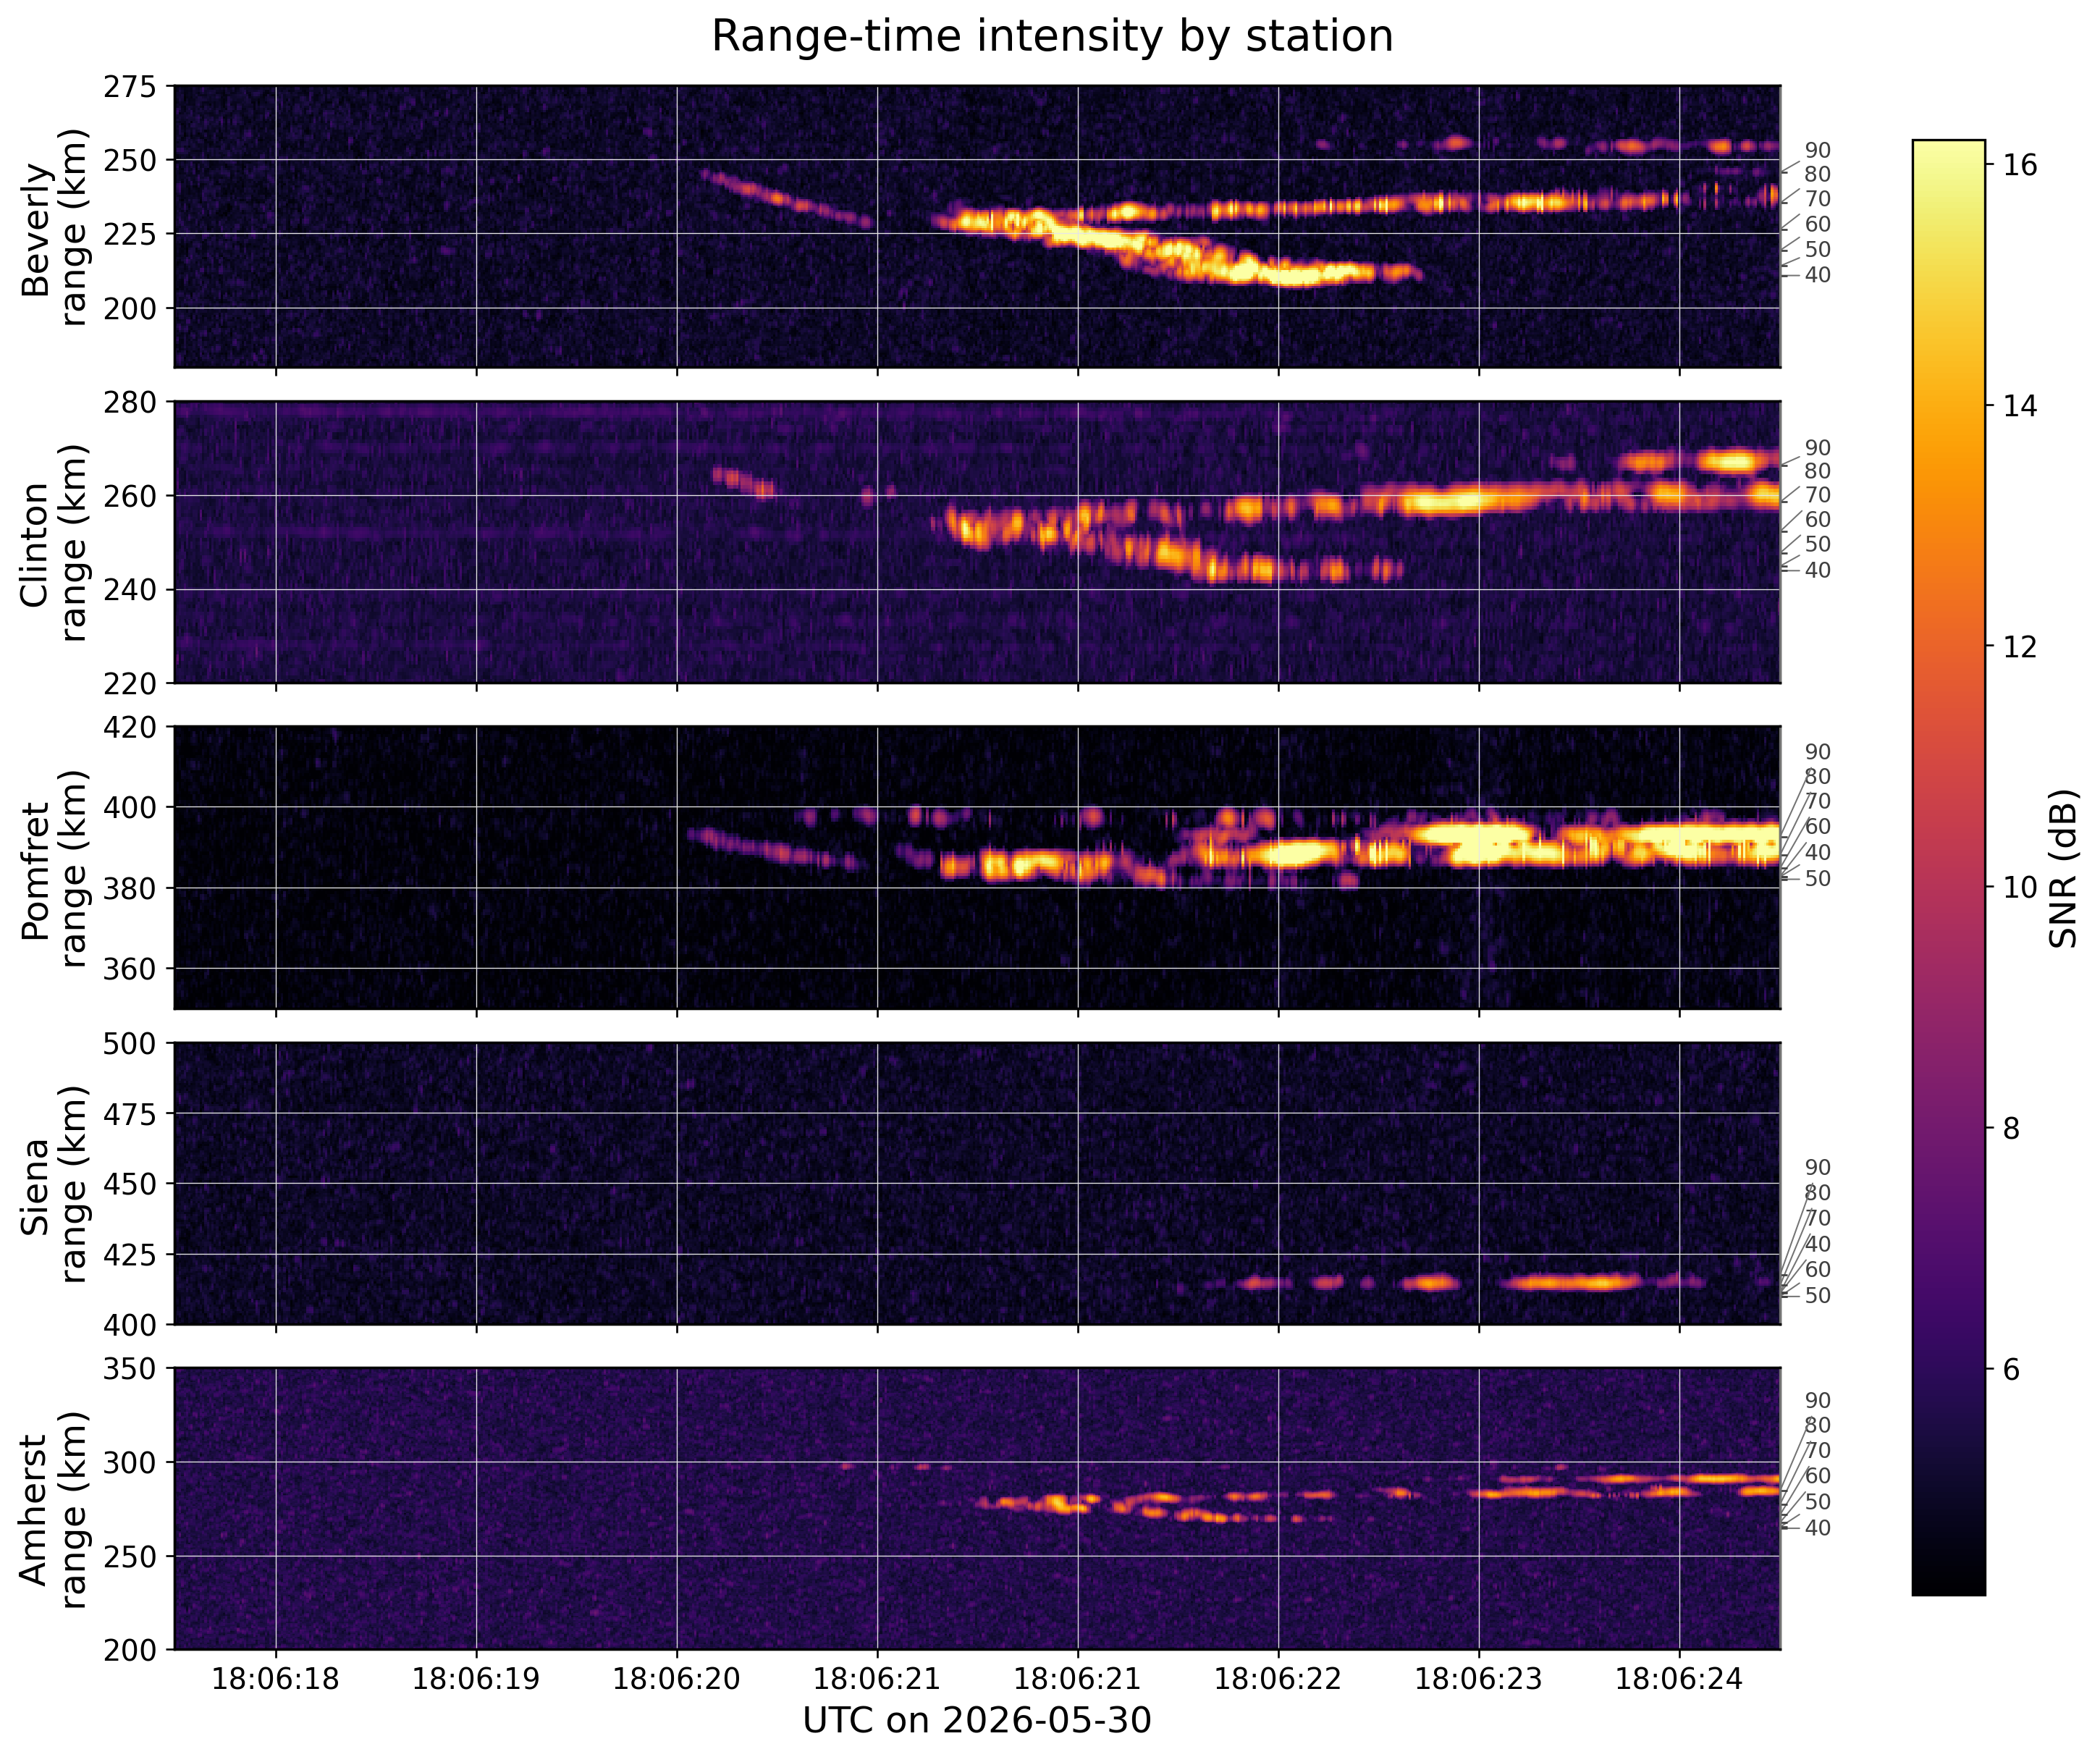
\includegraphics[width=\linewidth]{figures/station_range_time_snr.png}
  \caption{Range--time intensity for all five stations over the
  high-resolution 18:06:18--18:06:25 UTC interval.  The plotted range windows
  are Beverly 180--275 km, Clinton 220--280 km, Pomfret 350--420 km, Siena
  400--500 km, and Amherst 200--350 km.  The right-side manual labels mark the
  meteor altitude inferred from the fitted head-echo trajectory at the
  corresponding bistatic range for each station.}
  \figsource{reports/generate_station_rti_figures.py}
  \label{fig:station-rti-snr}
\end{figure}

\begin{figure}[ht]
  \centering
  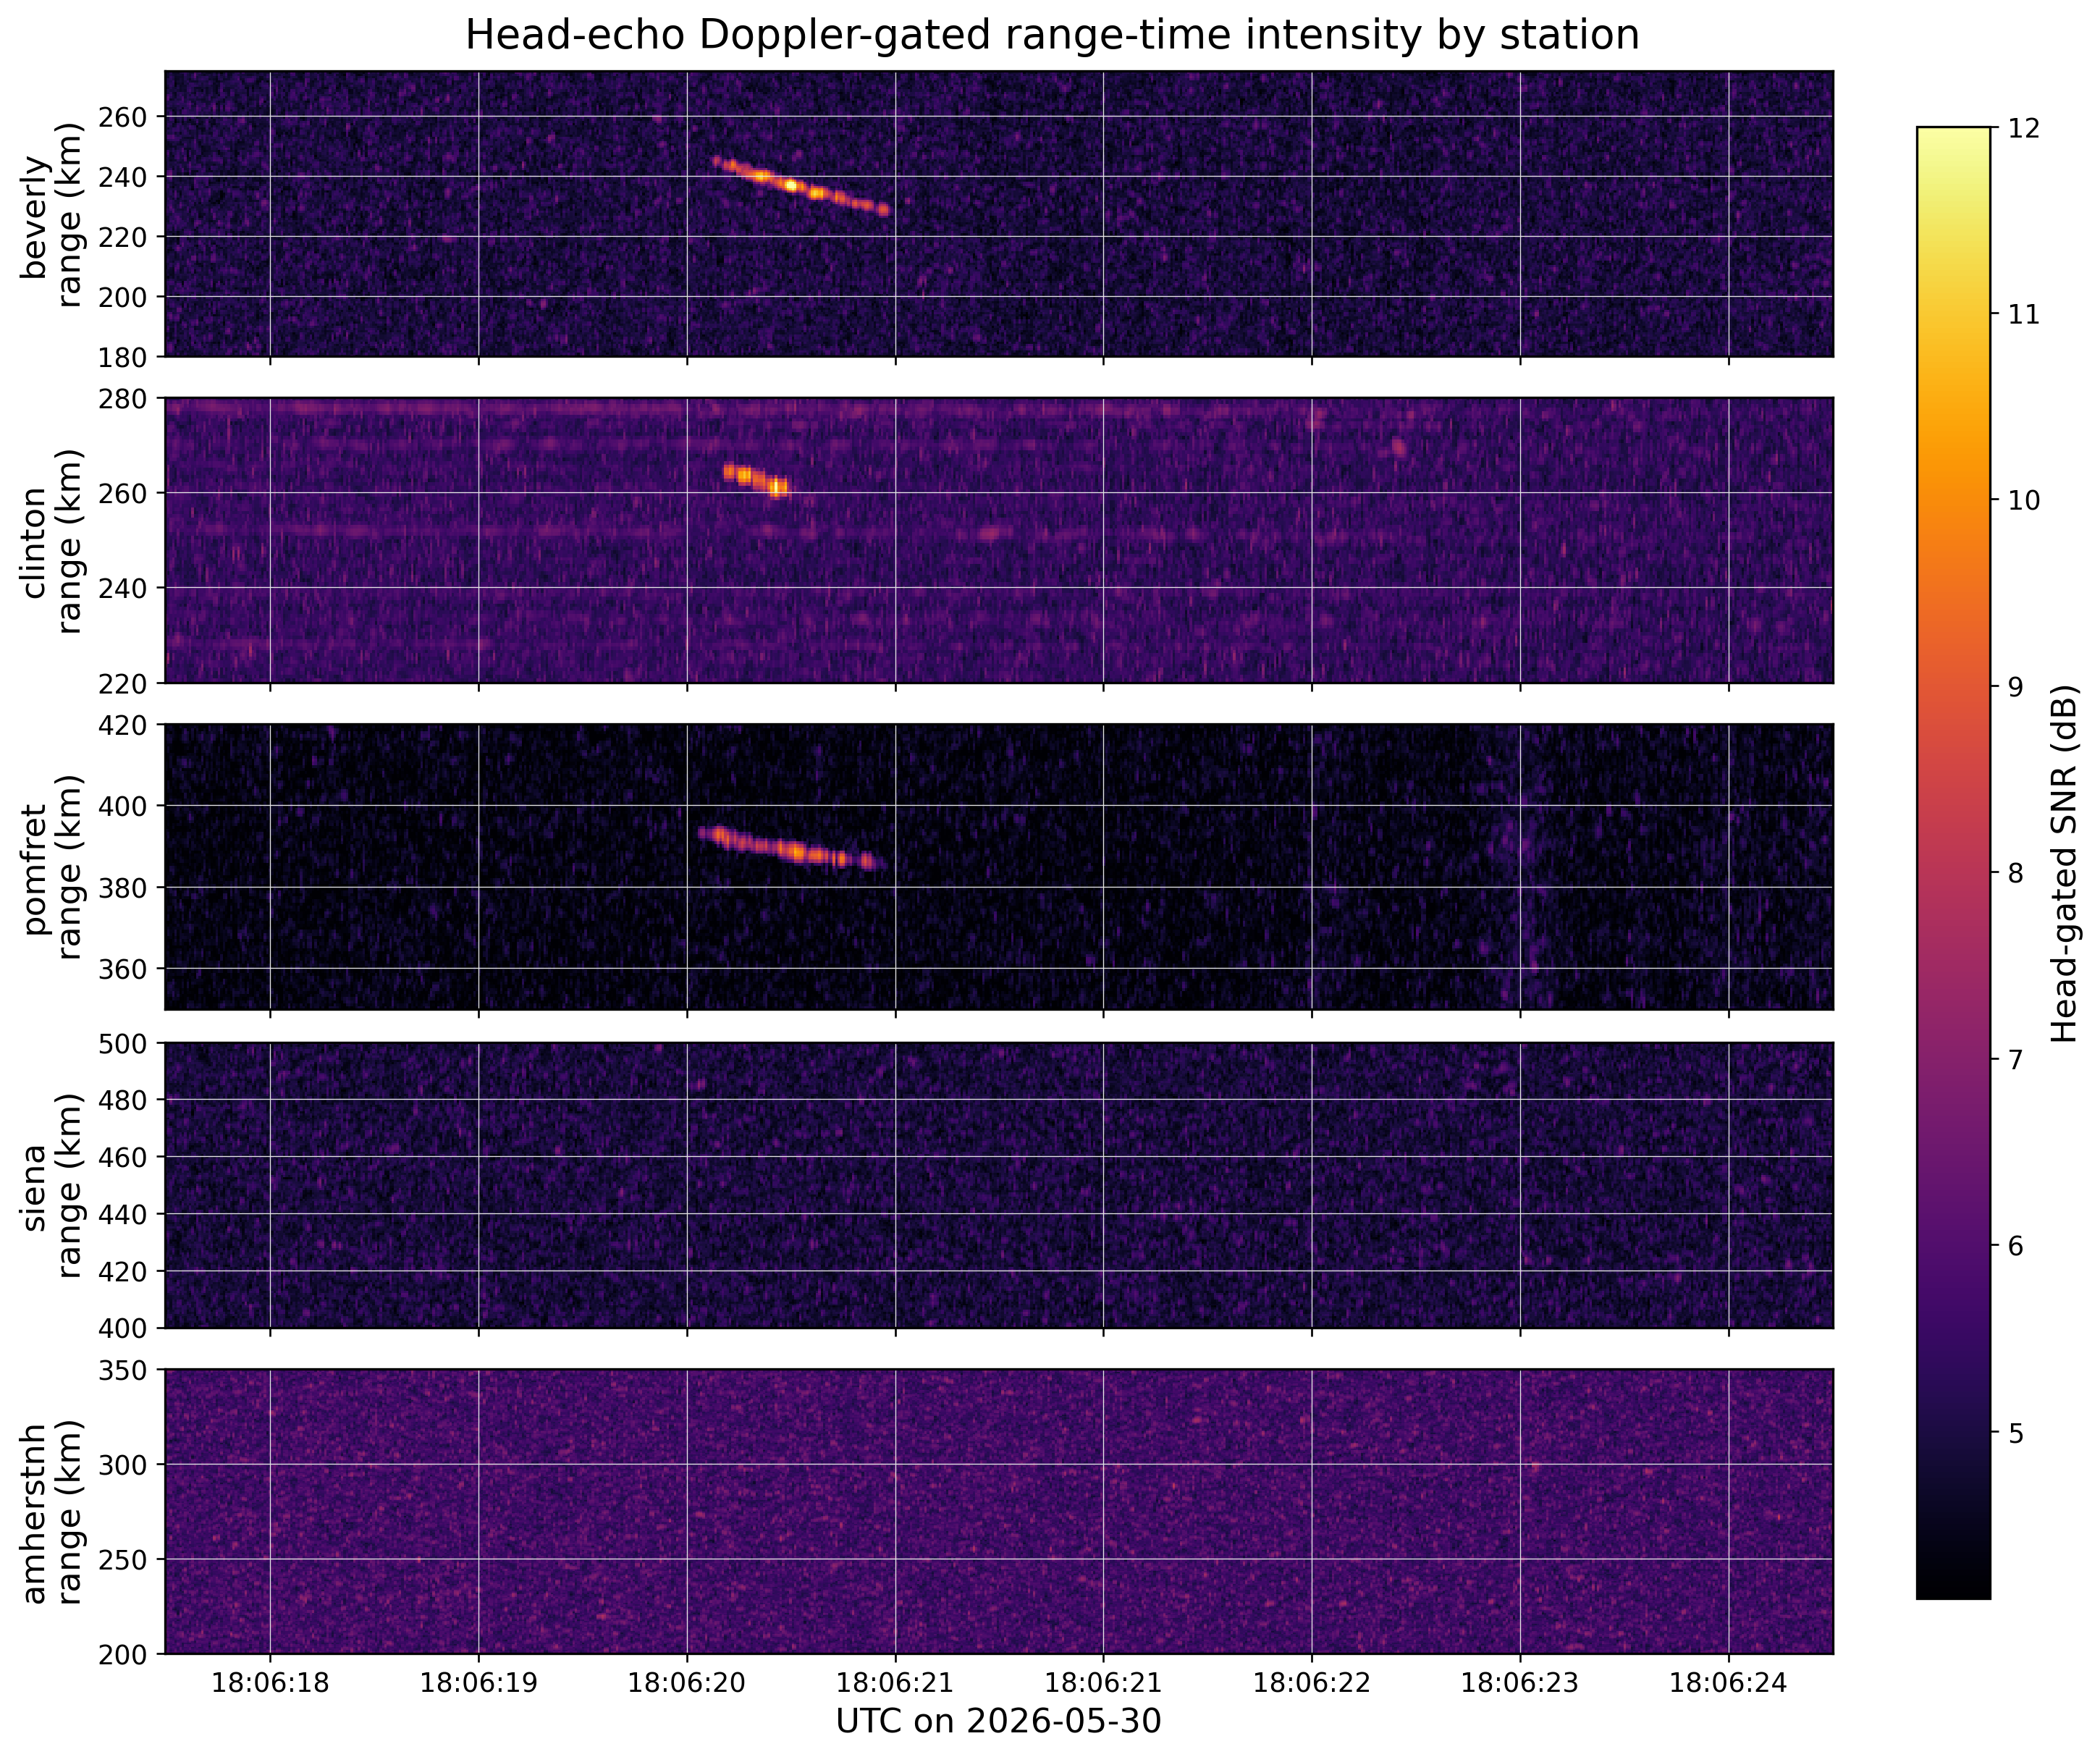
\includegraphics[width=\linewidth]{figures/station_range_time_head_snr.png}
  \caption{Range--time SNR from 18:06:19 to 18:06:22 UTC over the same
  station range windows as Figure~\ref{fig:station-rti-snr}, but using the
  meteor head-echo Doppler selection criterion.  At each time and range gate,
  the plotted SNR is the peak selected after requiring \(|f_D| \ge 250\) Hz,
  suppressing the near-zero-Doppler trail/clutter bins emphasized in the
  all-Doppler RTI.}
  \figsource{reports/generate_station_rti_figures.py}
  \label{fig:station-rti-head-snr}
\end{figure}

\begin{figure}[ht]
  \centering
  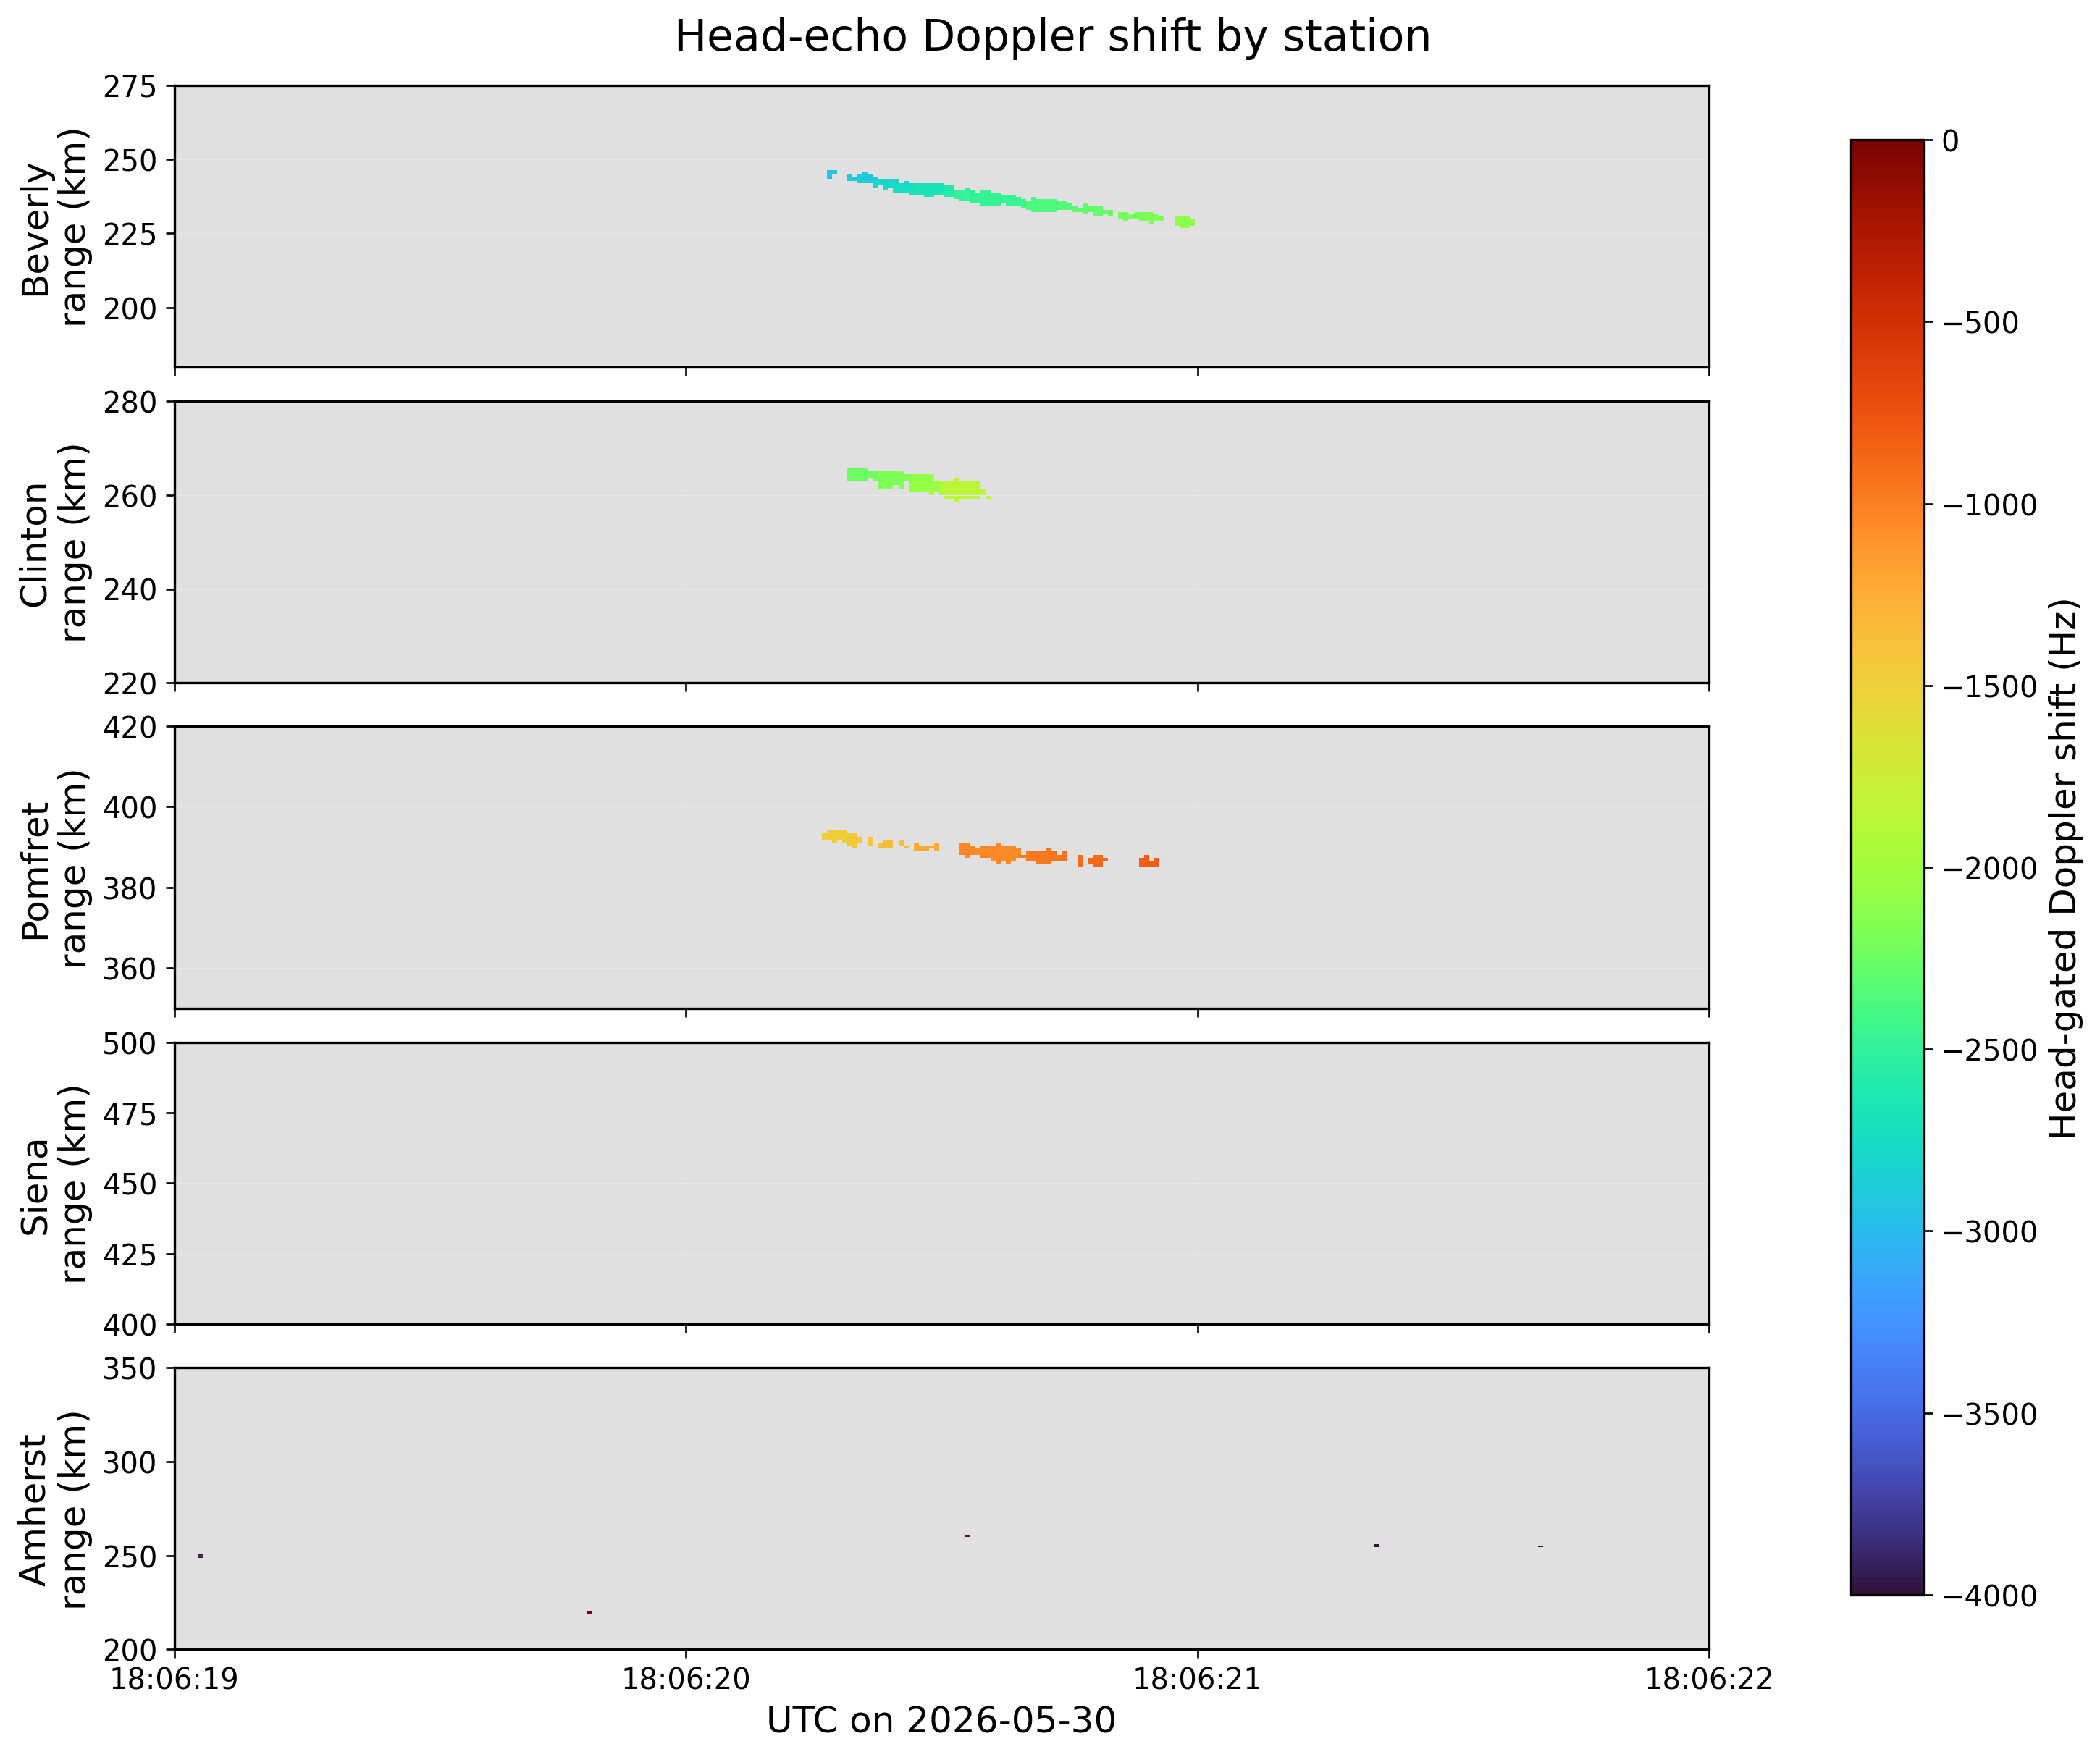
\includegraphics[width=\linewidth]{figures/station_range_time_head_doppler.png}
  \caption{Doppler shift from 18:06:19 to 18:06:22 UTC for the same
  head-echo-selected bins shown in Figure~\ref{fig:station-rti-head-snr}.
  Values are shown only where the head-gated SNR is at least 7.5 dB.}
  \figsource{reports/generate_station_rti_figures.py}
  \label{fig:station-rti-head-doppler}
\end{figure}

\begin{figure}[ht]
  \centering
  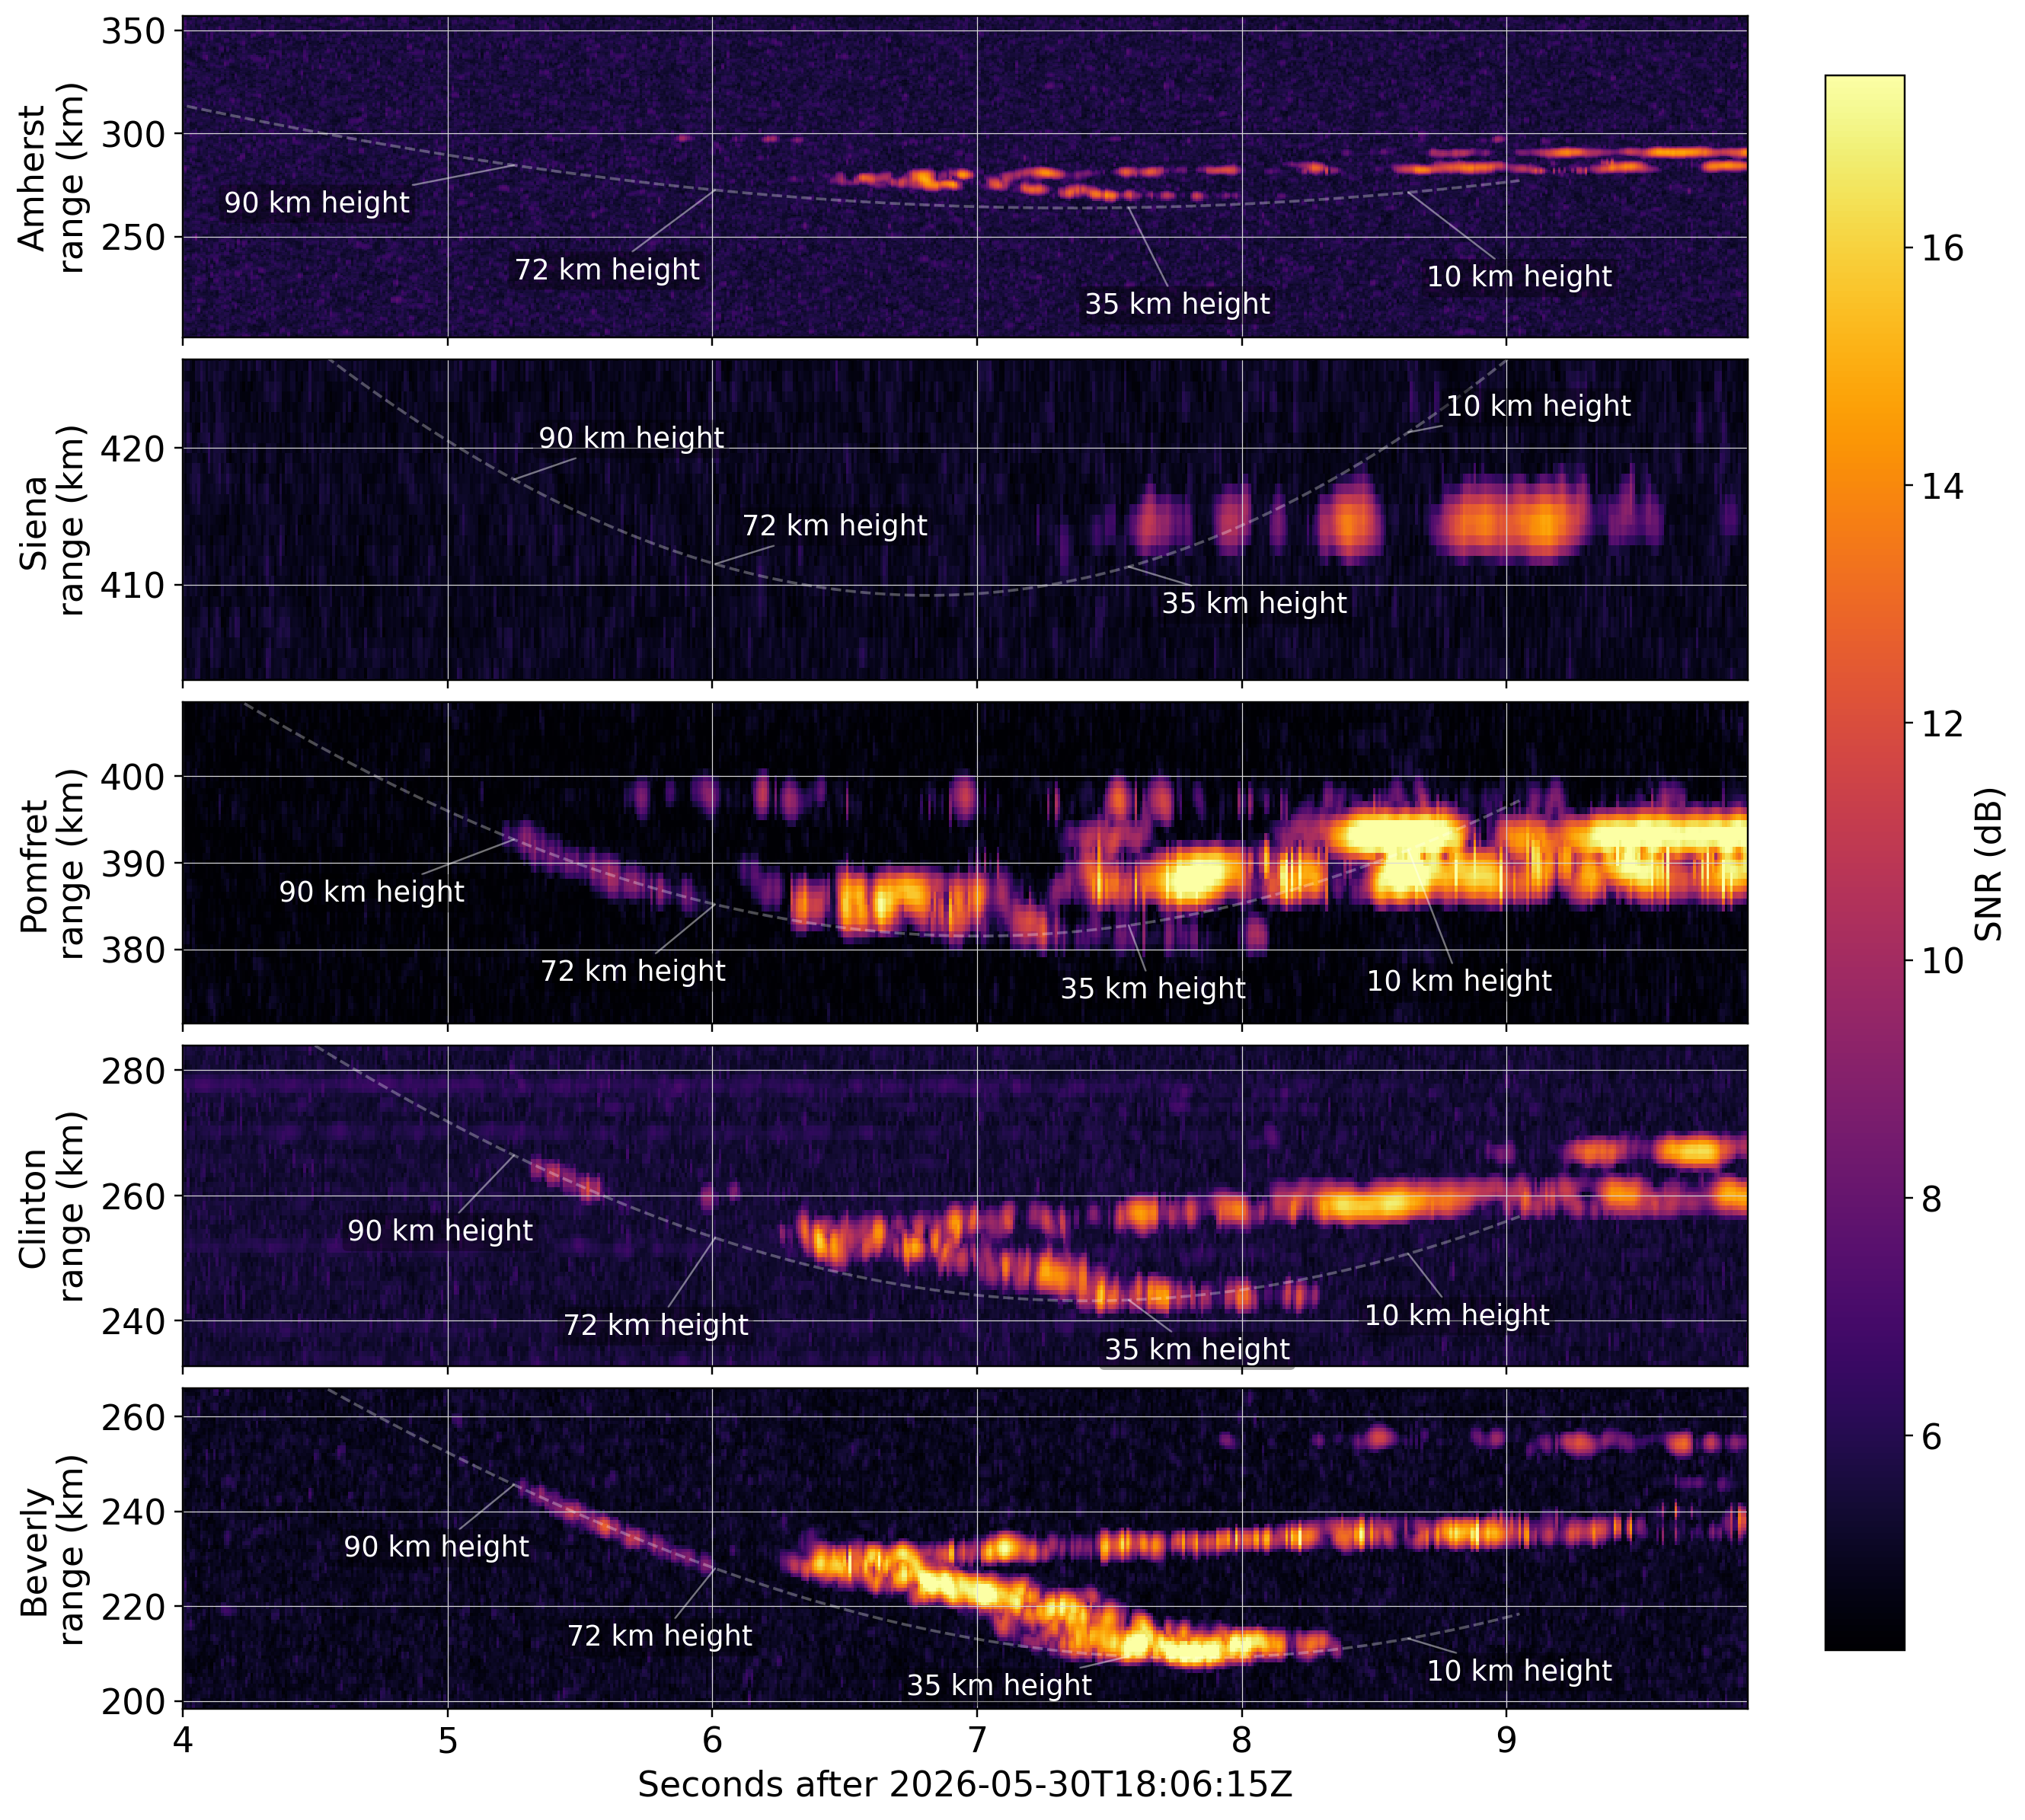
\includegraphics[width=\linewidth]{figures/trail_echo_roi.png}
  \caption{Near-zero-Doppler trail echo ROI for Amherst, Siena, Pomfret,
  Clinton, and Beverly.  The cyan contours mark cells with SNR at least 6 dB
  and \(|f_D| < 100\) Hz; all qualifying range gates are retained, so multiple
  range gates can contribute at one time step.  The right-side manual labels
  mark the meteor altitude inferred from the fitted head-echo trajectory at the
  corresponding bistatic range for each station.}
  \figsource{trail_echo_roi.py}
  \label{fig:trail-echo-roi}
\end{figure}

\section{Trajectory and Trail Echo Analysis}

The head-echo trajectory was determined from manually selected head-echo
regions in the Beverly, Clinton, and Pomfret range--Doppler products.  Within
each station region, one measurement was extracted at each time step by
choosing the range gate with the largest SNR, subject to a minimum SNR of
5 dB.  Robust outlier rejection was then applied independently to each
station's delay and Doppler sequence.  The first
\TrajectoryPomfretStartTrimS{} s of Pomfret measurements were excluded because
these earliest picks are inconsistent with the subsequent Pomfret trend.  The
final fit contains \TrajectoryNObservations{} retained measurements and
excludes \TrajectoryNRejected{} ROI peak measurements as outliers or
station-start trimmed points.

The fitted state is a six-parameter straight-line trajectory in the local ENU
frame of the transmitter,
\[
  {\bf x}(t) = {\bf x}_0 + {\bf v}(t-t_0).
\]
with both bistatic delay and bistatic Doppler fit simultaneously.  For each
transmitter--meteor--receiver path, the delay model is
\[
  \tau(t)=\frac{|{\bf x}(t)-{\bf x}_{\mathrm{tx}}|
             +|{\bf x}(t)-{\bf x}_{\mathrm{rx}}|}{c},
\]
and the bistatic Doppler model is
\[
  f_D(t)=\frac{f_0}{c}
  \left[
    \frac{{\bf x}(t)-{\bf x}_{\mathrm{tx}}}
         {|{\bf x}(t)-{\bf x}_{\mathrm{tx}}|}
    +
    \frac{{\bf x}(t)-{\bf x}_{\mathrm{rx}}}
         {|{\bf x}(t)-{\bf x}_{\mathrm{rx}}|}
  \right]\cdot{\bf v}(t).
\]
With this sign convention, positive Doppler corresponds to an increasing total
bistatic propagation path.
The residual RMS values for the current fit are \TrajectoryRangeRmsM{} m in
bistatic range and \TrajectoryDopplerRmsHz{} Hz in Doppler.
The uncertainty calculation uses the Jacobian from the nonlinear
least-squares fit.  If \({\bf p}\) is the six-component ENU state vector at
the reference time, consisting of position and velocity, the formal
least-squares parameter covariance is
\[
  {\bf C}_{p,\mathrm{formal}}=s^2\left({\bf J}^{T}{\bf J}\right)^{-1},
\]
with the inverse evaluated as a pseudo-inverse and \(s^2\) estimated from the
post-fit residual variance.  The adopted covariance used for all uncertainty
propagation is then recomputed with the physical range/Doppler Jacobian and
station-specific effective measurement scales
\[
  \sigma_{\mathrm{eff}}^2 =
  \sigma_{\mathrm{nominal}}^2+\sigma_{\mathrm{residual}}^2 ,
\]
where \(\sigma_{\mathrm{residual}}\) is the robust post-fit residual scatter
for the corresponding station and observable.  This folds the empirical
residual width back into the parameter covariance rather than using it only as
a plotting adjustment.  The same residual-derived scales are also applied to a
second trajectory-fit iteration.  In that second pass, the range/Doppler
residuals are divided by effective standard deviations of
982.6 m/502.6 Hz for Beverly, 945.1 m/515.4 Hz for Clinton, and
820.9 m/501.8 Hz for Pomfret.  These values define the relative weighting in
the whitened least-squares objective; the weights are the inverse variances in
the native units of each observable.  The second pass changes the residual RMS
from 475 m and 90 Hz to \TrajectoryRangeRmsM{} m and
\TrajectoryDopplerRmsHz{} Hz for range and Doppler, respectively.
The shaded bands in
Figure~\ref{fig:trajectory-observables} are prediction intervals: Monte Carlo
draws from the inflated \(\mathcal{N}({\bf p},{\bf C}_{p})\) are propagated
through the range and Doppler equations and then broadened by the empirical
95\% residual scatter for each station.

\begin{figure}[ht]
  \centering
  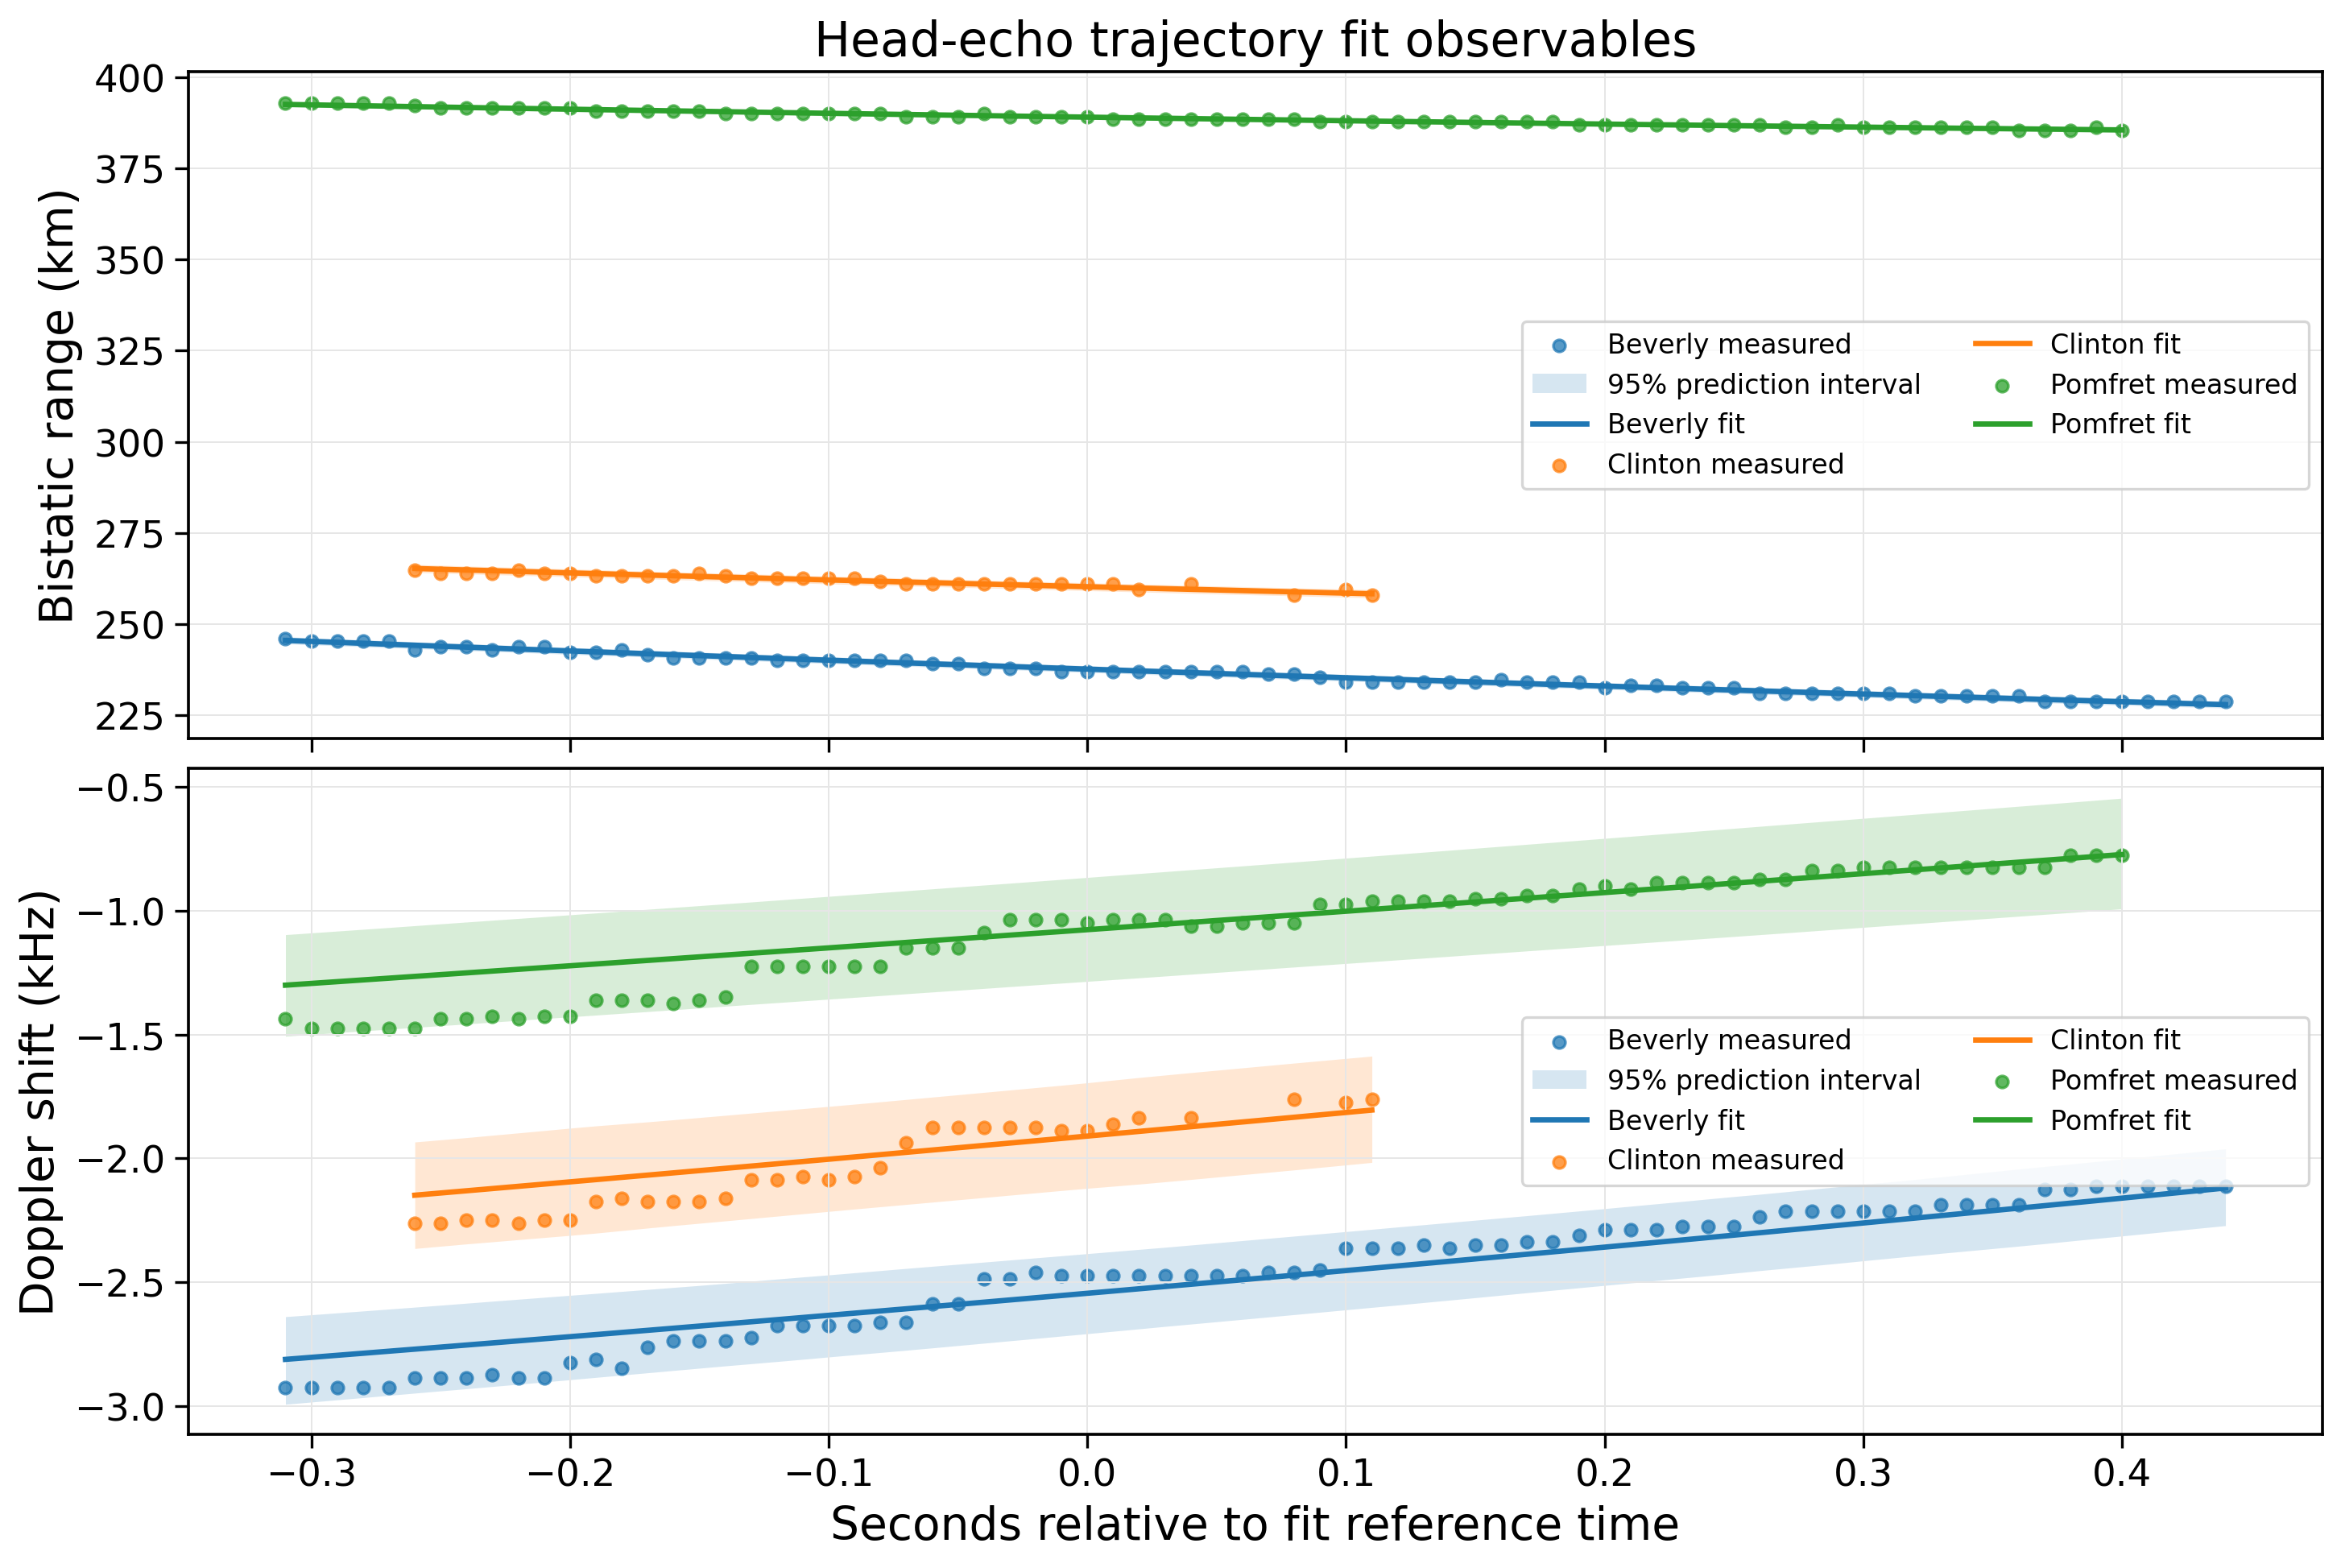
\includegraphics[width=\linewidth]{figures/head_echo_range_doppler_fit.png}
  \caption{Range and Doppler measurements used in the head-echo trajectory
  fit.  Points show the ROI-derived measurements after SNR thresholding and
  outlier rejection; lines show the fitted straight-line trajectory model for
  each bistatic path.  Shaded bands show 95\% prediction intervals formed by
  combining the sampled linearized parameter covariance with the empirical
  post-fit range and Doppler residual scatter.}
  \figsource{reports/generate_trajectory_report_assets.py}
  \label{fig:trajectory-observables}
\end{figure}

The first retained detection occurred at \TrajectoryFirstDetectionUTC{}.  The
best-fit initial detection height was \TrajectoryInitialHeightKm{} km at
latitude \TrajectoryInitialLat{} deg and longitude \TrajectoryInitialLon{} deg.
The fitted initial velocity is
\[
  {\bf v}_{\mathrm{ENU}} =
  (\TrajectoryVEastKmS{},\ \TrajectoryVNorthKmS{},\ \TrajectoryVUpKmS{})
  \ \mathrm{km\,s^{-1}},
\]
with speed \TrajectorySpeedKmS{} km s\(^{-1}\).  The large negative upward
component is consistent with a steeply descending trajectory during the
head-echo interval.  The corresponding apparent radiant, without
zenithal-attraction correction, is RA
\(\TrajectoryRadiantRADeg{}\pm\TrajectoryRadiantRASigmaDeg{}\) deg, Dec
\(\TrajectoryRadiantDecDeg{}\pm\TrajectoryRadiantDecSigmaDeg{}\) deg, or Az
\(\TrajectoryRadiantAzDeg{}\pm\TrajectoryRadiantAzSigmaDeg{}\) deg, El
\(\TrajectoryRadiantElDeg{}\pm\TrajectoryRadiantElSigmaDeg{}\) deg in the
local horizon frame at the first detection point.  The quoted speed
uncertainty is \(\TrajectorySpeedSigmaKmS{}\) km s\(^{-1}\), computed from the
same covariance samples.

\begin{figure}[ht]
  \centering
  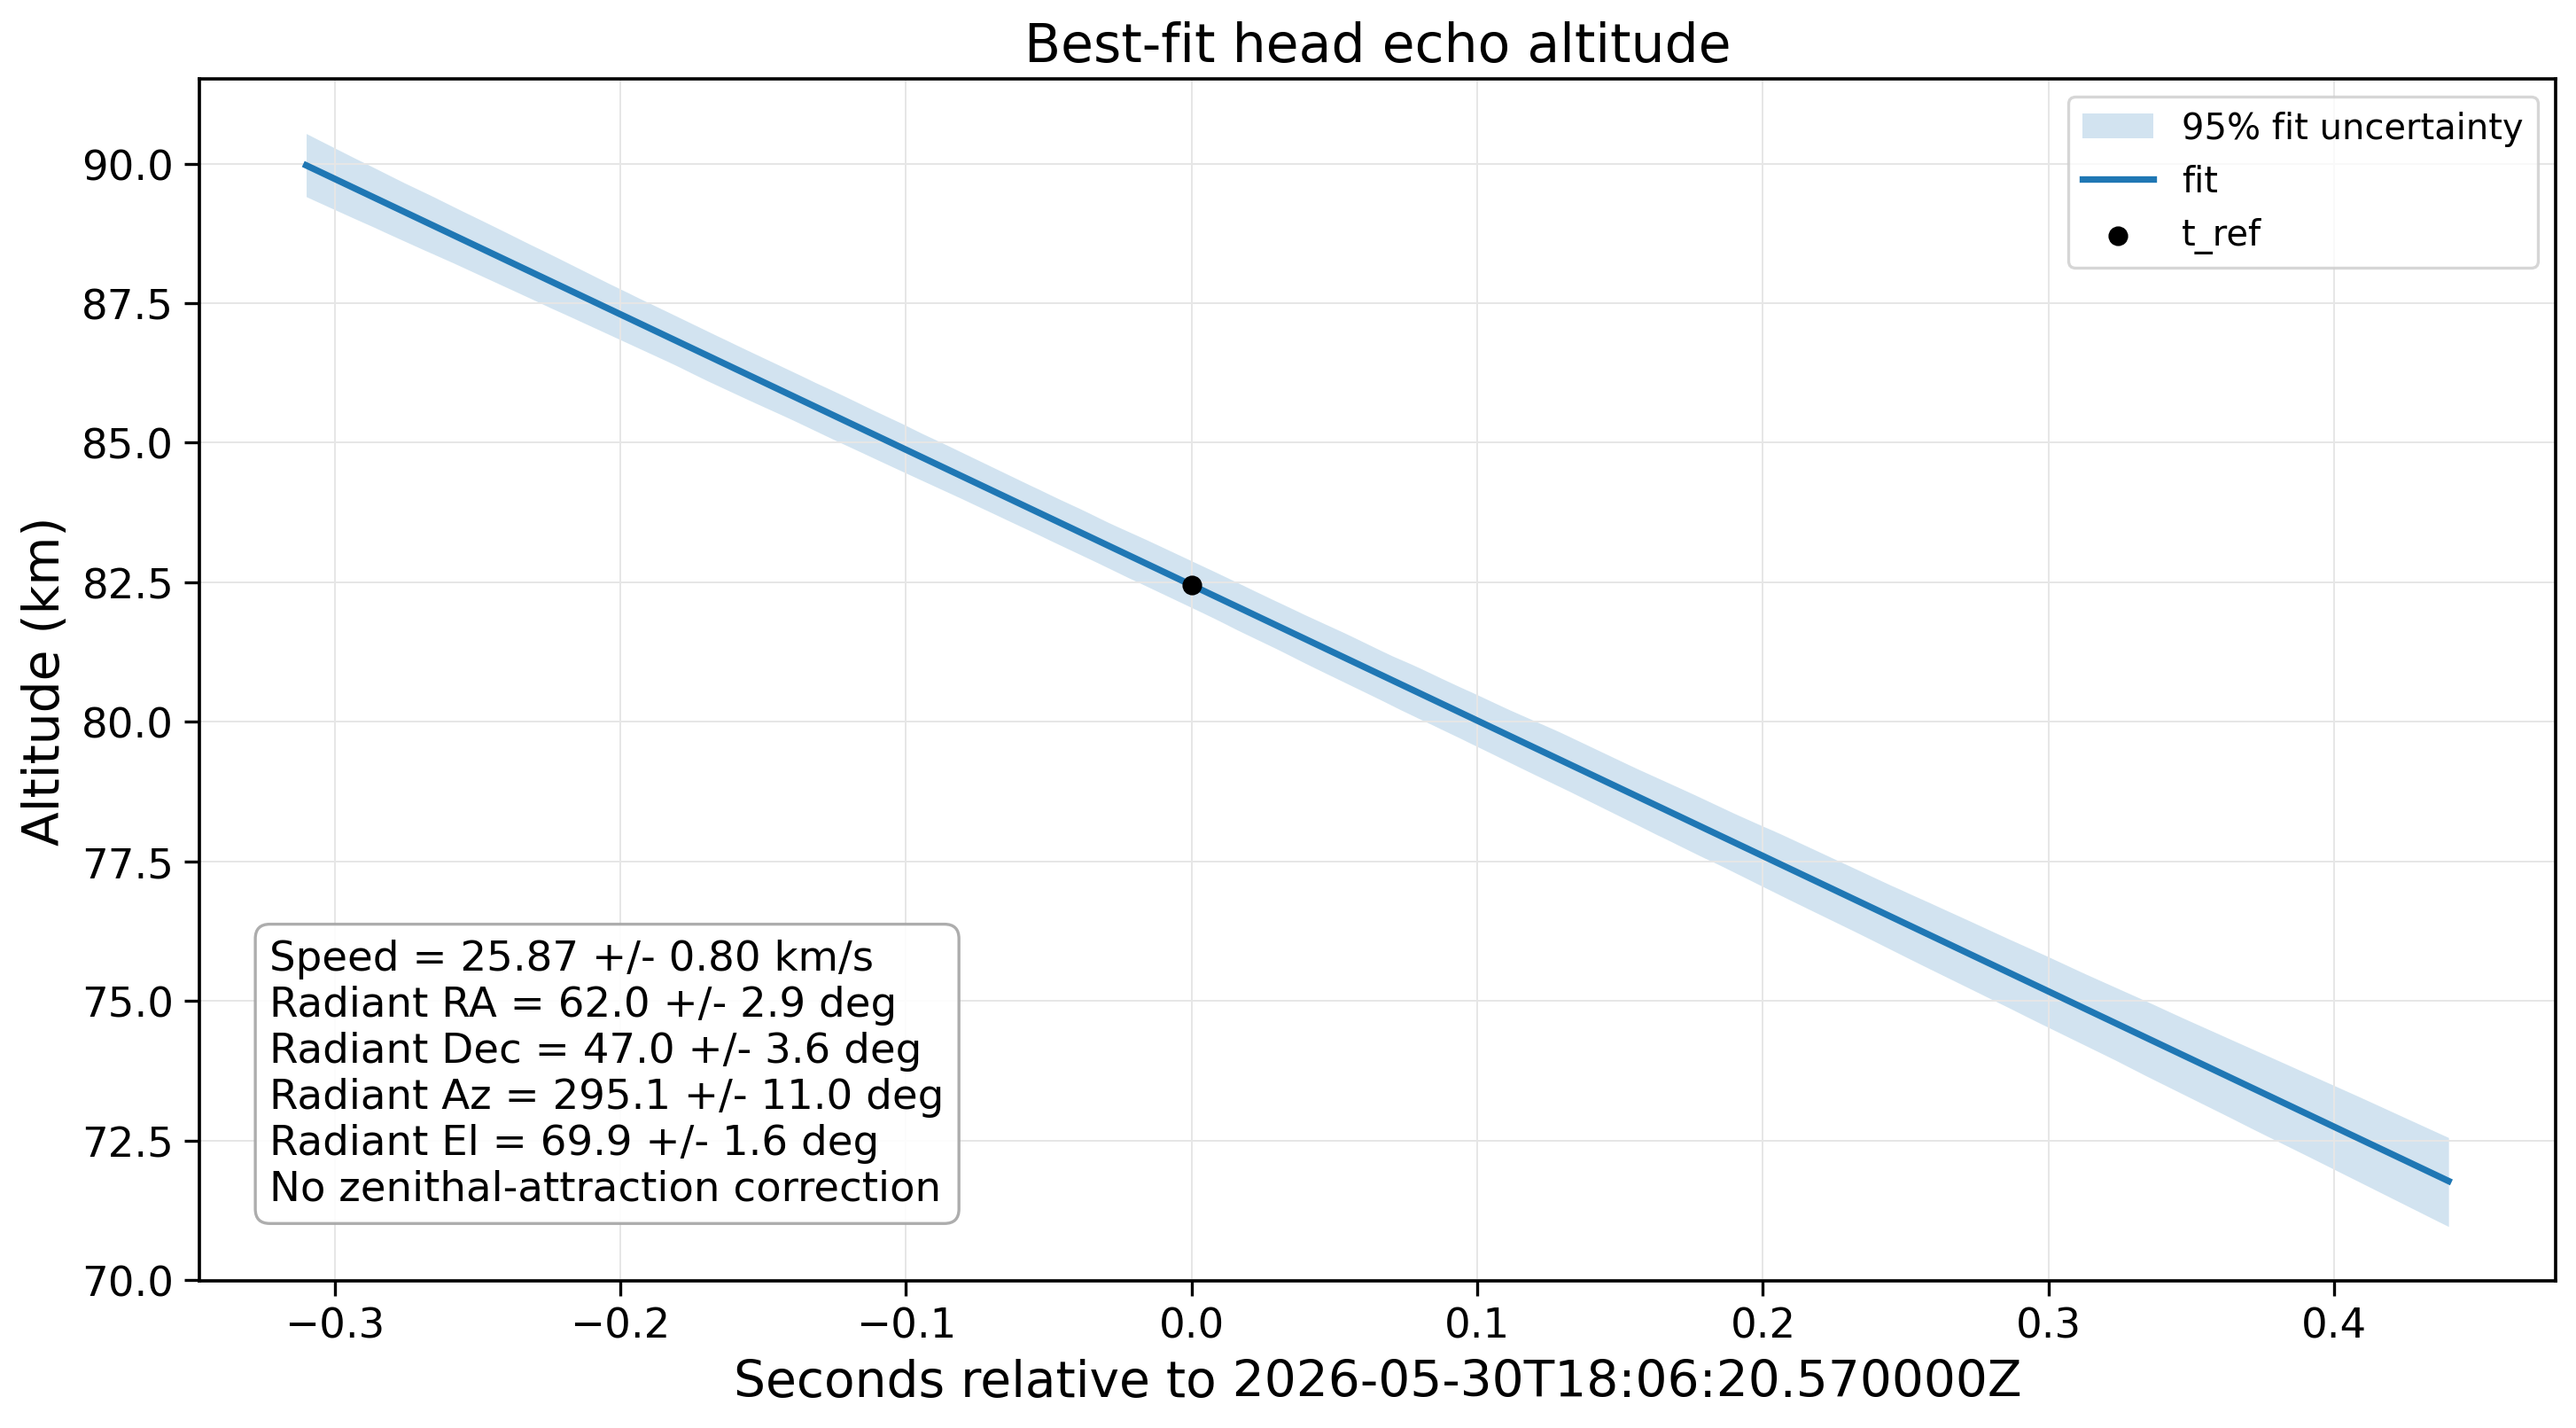
\includegraphics[width=\linewidth]{figures/head_echo_altitude_velocity.png}
  \caption{Altitude implied by the straight-line fit over the retained
  head-echo detection interval.  The text inset gives the fitted absolute
  speed and apparent radiant in RA/Dec and Az/El, including 1-sigma
  uncertainty from covariance samples.  No zenithal-attraction correction has
  been applied.  Shaded bands show sampled 95\% fit uncertainty from the
  linearized least-squares covariance.}
  \figsource{reports/generate_trajectory_report_assets.py}
  \label{fig:trajectory-altitude}
\end{figure}

A second trajectory solution was computed in an inertial frame by combining
the timed head-echo range/Doppler measurements with the non-specular trail echo
positions.  The frame transformation uses a fast Greenwich mean sidereal time
rotation between ECEF and ECI coordinates; the full Astropy GCRS/ITRS
transformation is unnecessary over this several-second arc and is too slow for
iterating on the fit diagnostics.  Most trail echoes are treated as
point-on-path constraints only: the plasma position constrains the spatial
line followed by the meteoroid, but not the time at which the meteoroid passed
that point.  Below 60 km altitude, however, the non-specular trail echoes are
relatively prompt and decay quickly.  For those low-altitude trail points, the
fit also constrains the echo occurrence time to lag the meteoroid passage time
by \(1\pm1\) s.

The straight-line ECI state is
\({\bf p}=({\bf r}_0,{\bf v})\), and the fitted path is
\({\bf r}(t)={\bf r}_0+{\bf v}(t-t_0)\).  For head-echo measurement \(i\), the
model predicts bistatic range \(\rho_i({\bf p})\) and Doppler
\(f_i({\bf p})\).  For trail position \({\bf y}_j\), the closest-path time is
\[
  \tau_j =
  \frac{{\bf v}\cdot({\bf y}_j-{\bf r}_0)}{{\bf v}\cdot{\bf v}},
\]
and the point-to-path residual vector is
\[
  {\bf d}_j({\bf p}) =
  {\bf r}_0 + {\bf v}\tau_j - {\bf y}_j .
\]
The least-squares objective minimized after outlier rejection is
\[
  \begin{aligned}
  \chi^2({\bf p}) ={}&
    \sum_i \left[
      \frac{\rho_i({\bf p})-\rho_i^{\mathrm{obs}}}{\sigma_\rho}
    \right]^2
    +
    \sum_i \left[
      \frac{f_i({\bf p})-f_i^{\mathrm{obs}}}{\sigma_f}
    \right]^2 \\
  &+
    \sum_j
    \frac{\|{\bf d}_j({\bf p})\|^2}{\sigma_{\mathrm{trail}}^2}
    +
    \sum_{j:\,h_j<60\,\mathrm{km}}
    \left[
      \frac{t_j^{\mathrm{echo}}-(t_0+\tau_j+1\,\mathrm{s})}{1\,\mathrm{s}}
    \right]^2 .
  \end{aligned}
\]
The numerical solve uses a soft-\(\ell_1\) loss, but the covariance and plotted
uncertainty samples use the final linearized least-squares Jacobian.  The
measurement scales are estimated from the fit residuals and then applied in a
final fit iteration: \(\sigma_\rho=573\) m, \(\sigma_f=81\) Hz, and
\(\sigma_{\mathrm{trail}}=1.09\) km per trail-position component.  The
low-altitude timing term contributes 21 residuals.

The combined fit admits trail positions between 20 and 115 km altitude.  It
used 181 head-echo measurements and 139 trail positions; four trail positions
were rejected as line-distance outliers.  The resulting residual RMS values are
547 m in head-echo range and 80 Hz in head-echo Doppler, while the retained
trail positions have a median perpendicular distance of 1.49 km and a 95th
percentile distance of 3.88 km.

A physically motivated ballistic propagation fit was then computed by replacing
the straight-line motion model with central Earth gravity and atmospheric drag.
The fitted state is \({\bf y}=({\bf r},{\bf v})\), propagated according to
\[
  \begin{aligned}
    \dot{\bf r} &= {\bf v},\\
    \dot{\bf v} &=
      -\frac{\mu_E}{\|{\bf r}\|^3}{\bf r}
      -\frac{1}{2}\rho(h)\frac{C_D A}{m}
      \|{\bf v}-{\bf v}_{\mathrm{atm}}\|
      ({\bf v}-{\bf v}_{\mathrm{atm}}),
  \end{aligned}
\]
where \({\bf v}_{\mathrm{atm}}={\boldsymbol\omega}_E\times{\bf r}\) assumes a
co-rotating atmosphere.  The atmospheric density \(\rho(h)\) is taken from an
MSIS altitude profile when available, with an exponential fallback.  The
optimized drag parameter is a single constant \(C_D A/m\), initialized from the
combined straight-line solution and fit together with the reference position
and velocity.  The fitted value is
\(C_D A/m = 8.45\times10^{-4}\ \mathrm{m^2\,kg^{-1}}\).  The retained trail
positions have a median distance of 1.81 km from the ballistic trajectory.

For the fall-line extrapolation, the fitted ballistic trajectory is propagated
to 30 km altitude.  The radar trail measurements near this altitude constrain
the position and direction of the path immediately before dark flight, but the
subsequent sea-level impact depends on the size distribution of surviving
fragments.  A nominal 10 cm diameter spherical fragment of density
\(3000\ \mathrm{kg\,m^{-3}}\) is used as a reference case.  With \(C_D=1\), this
gives
\[
  \frac{C_D A}{m}
  =
  \frac{3C_D}{2d\rho_m}
  =
  0.005\ \mathrm{m^2\,kg^{-1}} .
\]
In this nominal extrapolation, the trajectory reaches 30 km altitude at
18:06:22.75 UTC and the 10 cm fragment reaches sea level at 18:11:16.93 UTC
with a speed of about 351 m s\(^{-1}\).  To represent the unknown surviving
fragment size, Figure~\ref{fig:ballistic-impact-map} and
Table~\ref{tab:fragment-impact} also sample fragment diameters from 1 to
100 cm at fixed density, combined with samples from the linearized covariance
of the ballistic fit.  The resulting spread should be interpreted as a large
dark-flight uncertainty, not as a precise strewn-field prediction.

\begin{figure}[ht]
  \centering
  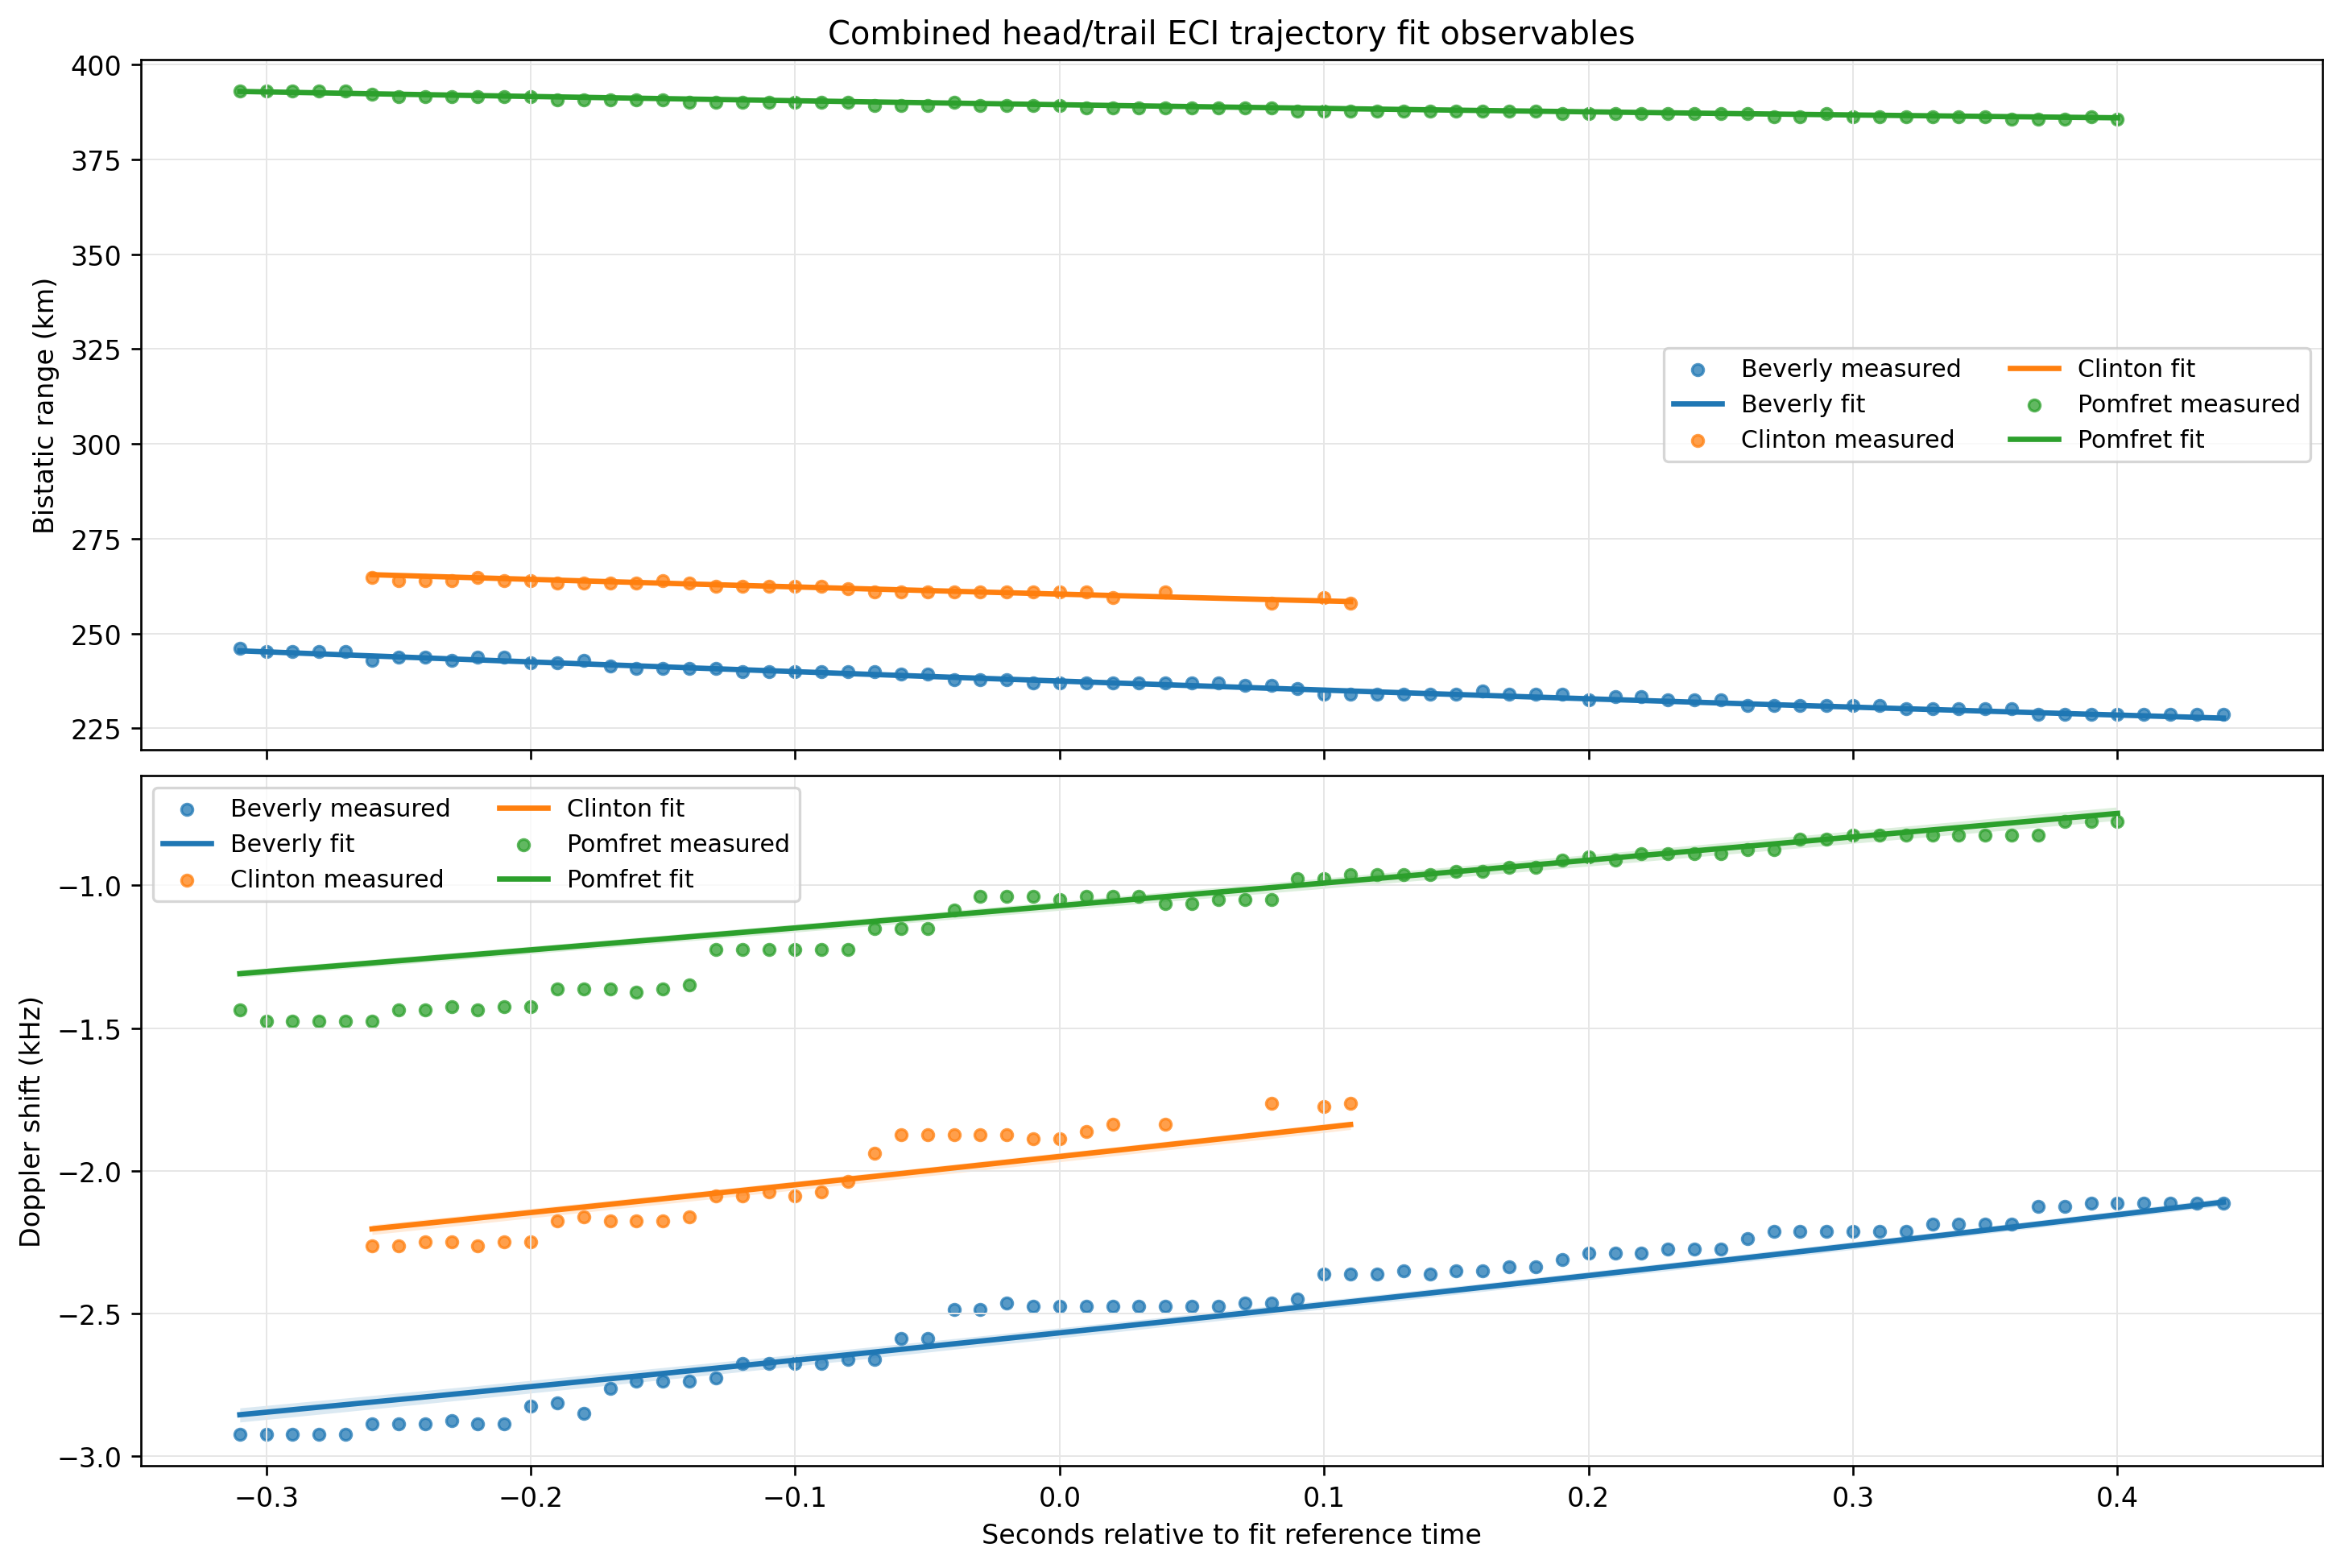
\includegraphics[width=\linewidth]{figures/combined_head_trail_range_doppler_fit.png}
  \caption{Range and Doppler measurements for the combined ECI head/trail
  trajectory fit.  Points show the timed head-echo measurements; lines show
  the fitted bistatic range and Doppler model.  Shaded bands show sampled
  95\% uncertainty from the combined-fit covariance.}
  \figsource{fit_combined_head_trail_eci.py}
  \label{fig:combined-trajectory-observables}
\end{figure}

\begin{figure}[ht]
  \centering
  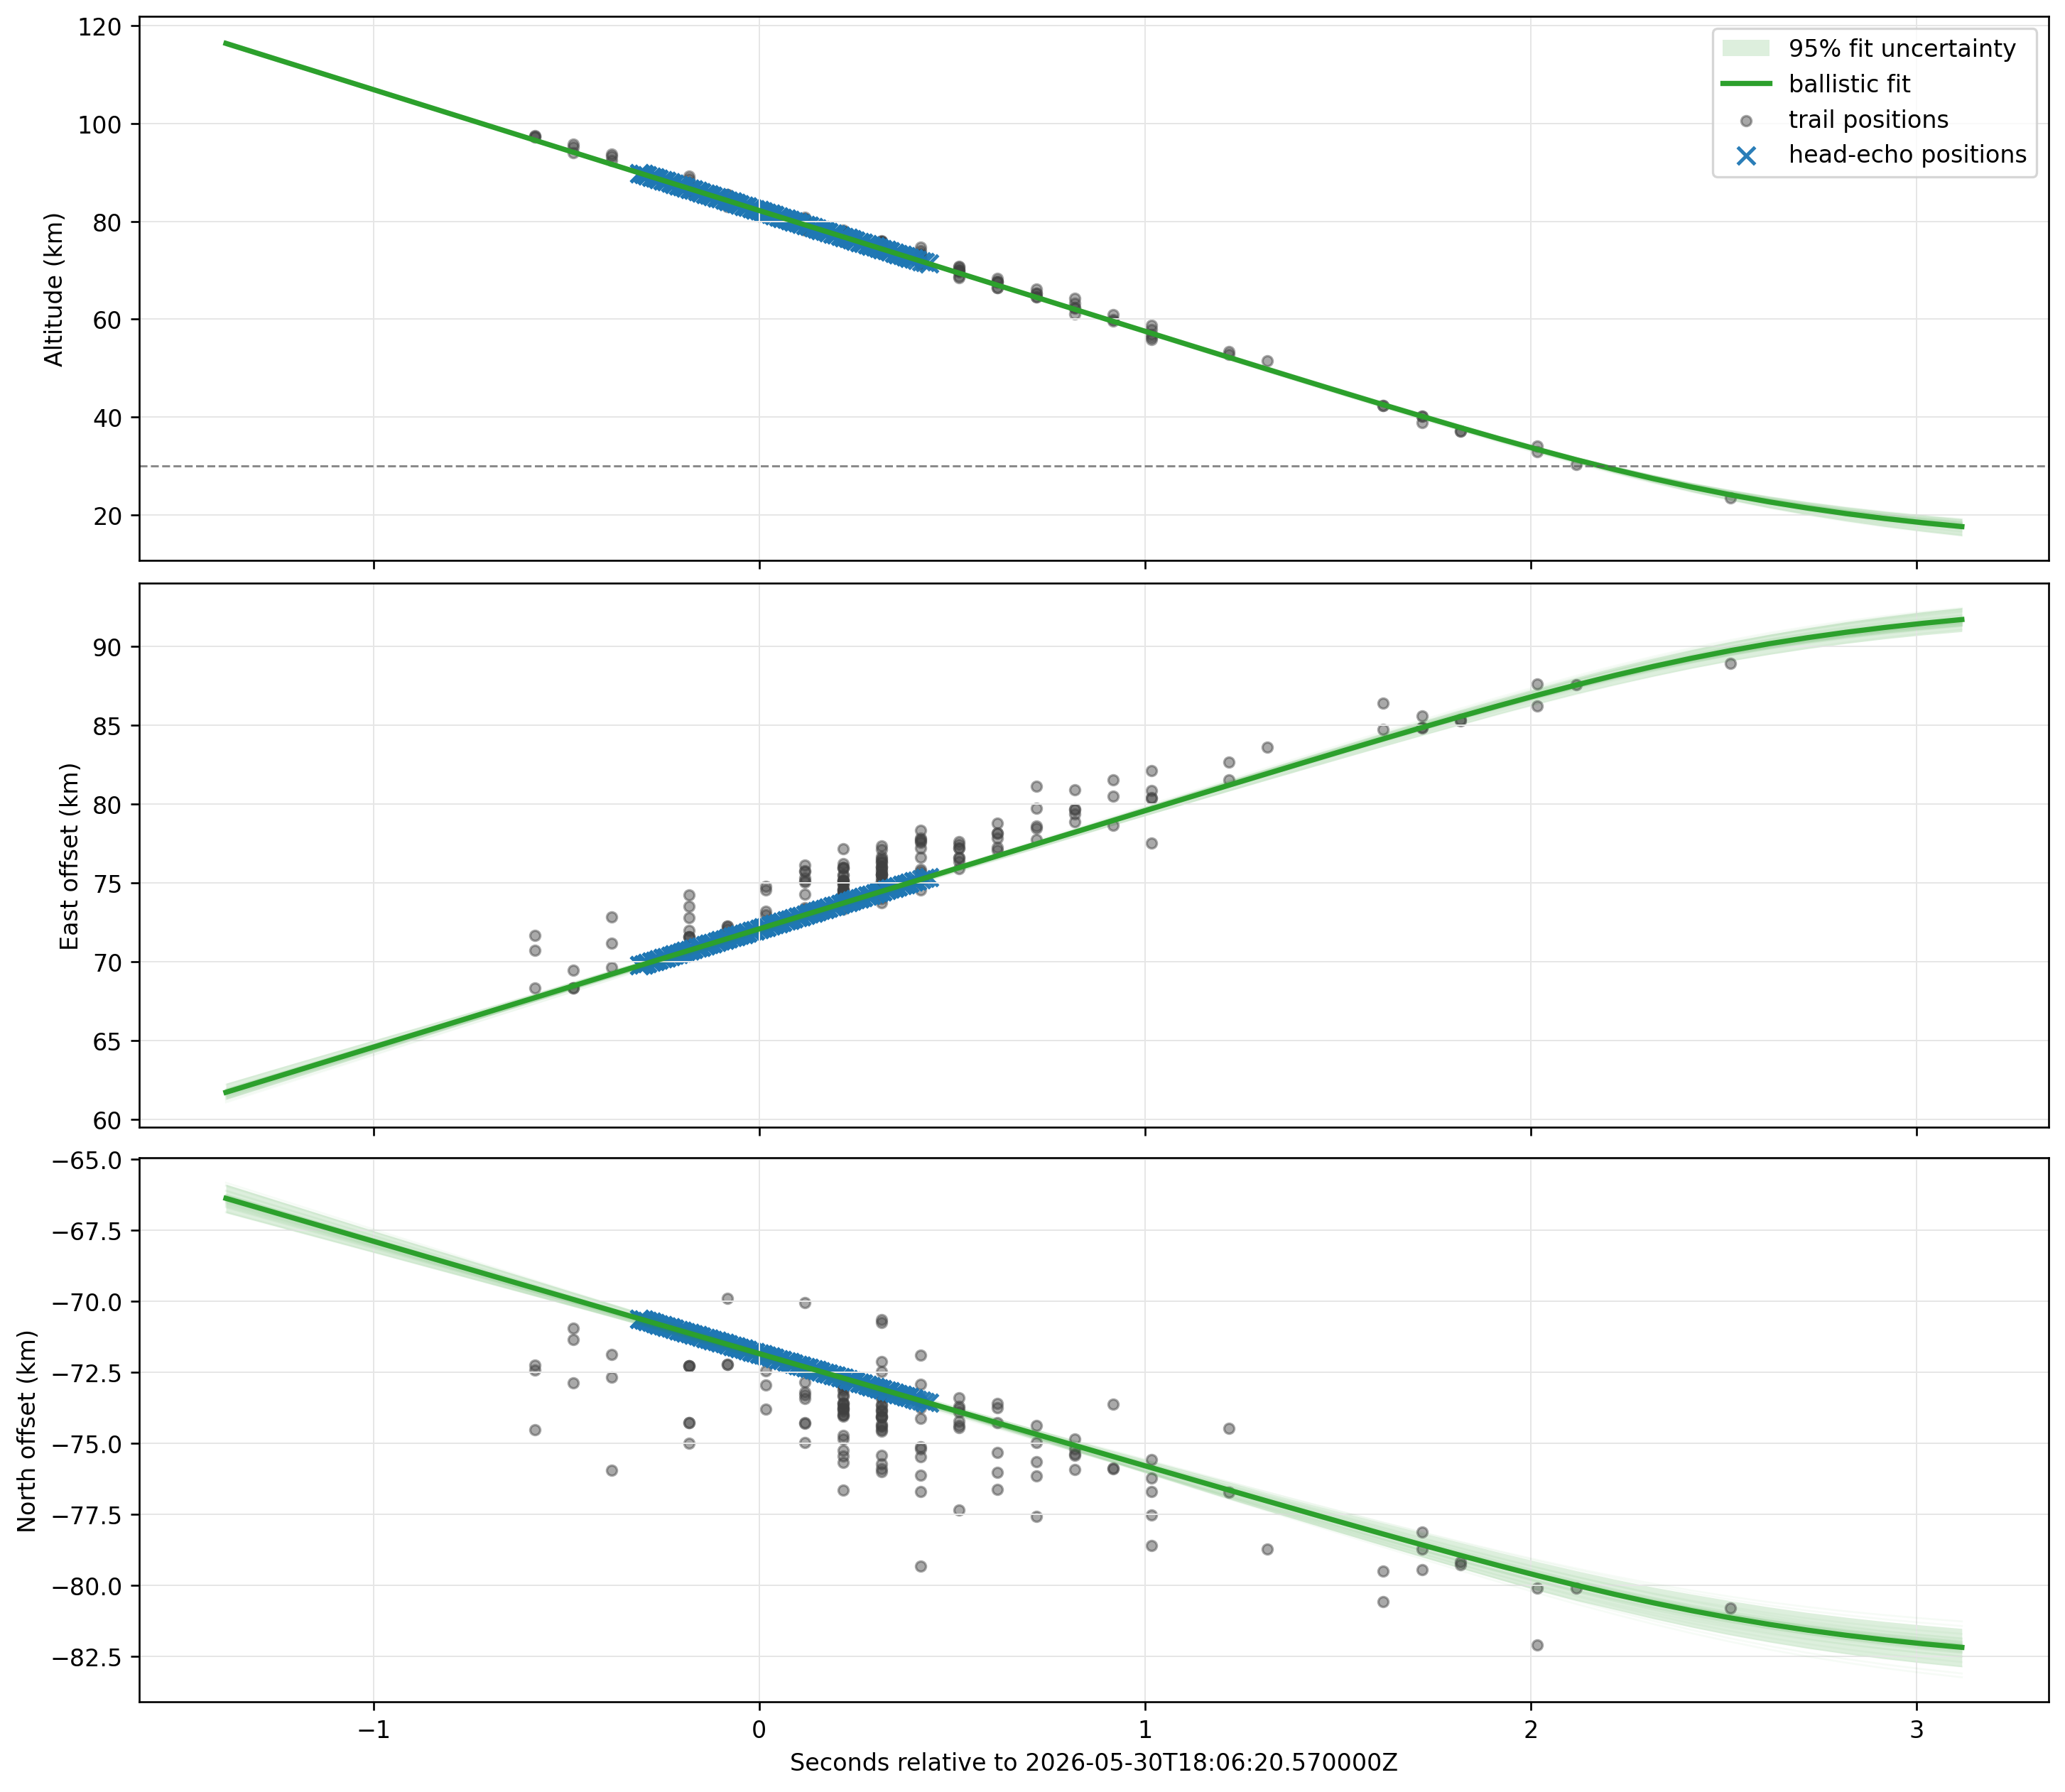
\includegraphics[width=\linewidth]{figures/ballistic_head_trail_altitude_enu.png}
  \caption{Ballistic trajectory in the transmitter ENU frame.  The green curve
  shows the best-fit ballistic trajectory through the head-echo and retained
  trail region; the shaded band and faint green curves show samples from the
  linearized fit covariance.  Blue crosses show head-echo-derived positions and
  gray points show non-specular trail positions projected to the closest point
  on the trajectory.  The dashed line marks 30 km altitude, where the nominal
  fragment model used for the impact estimate in Figure~\ref{fig:ballistic-impact-map}
  begins.}
  \figsource{fit_ballistic_head_trail.py}
  \label{fig:ballistic-trajectory-altitude}
\end{figure}

\begin{figure}[ht]
  \centering
  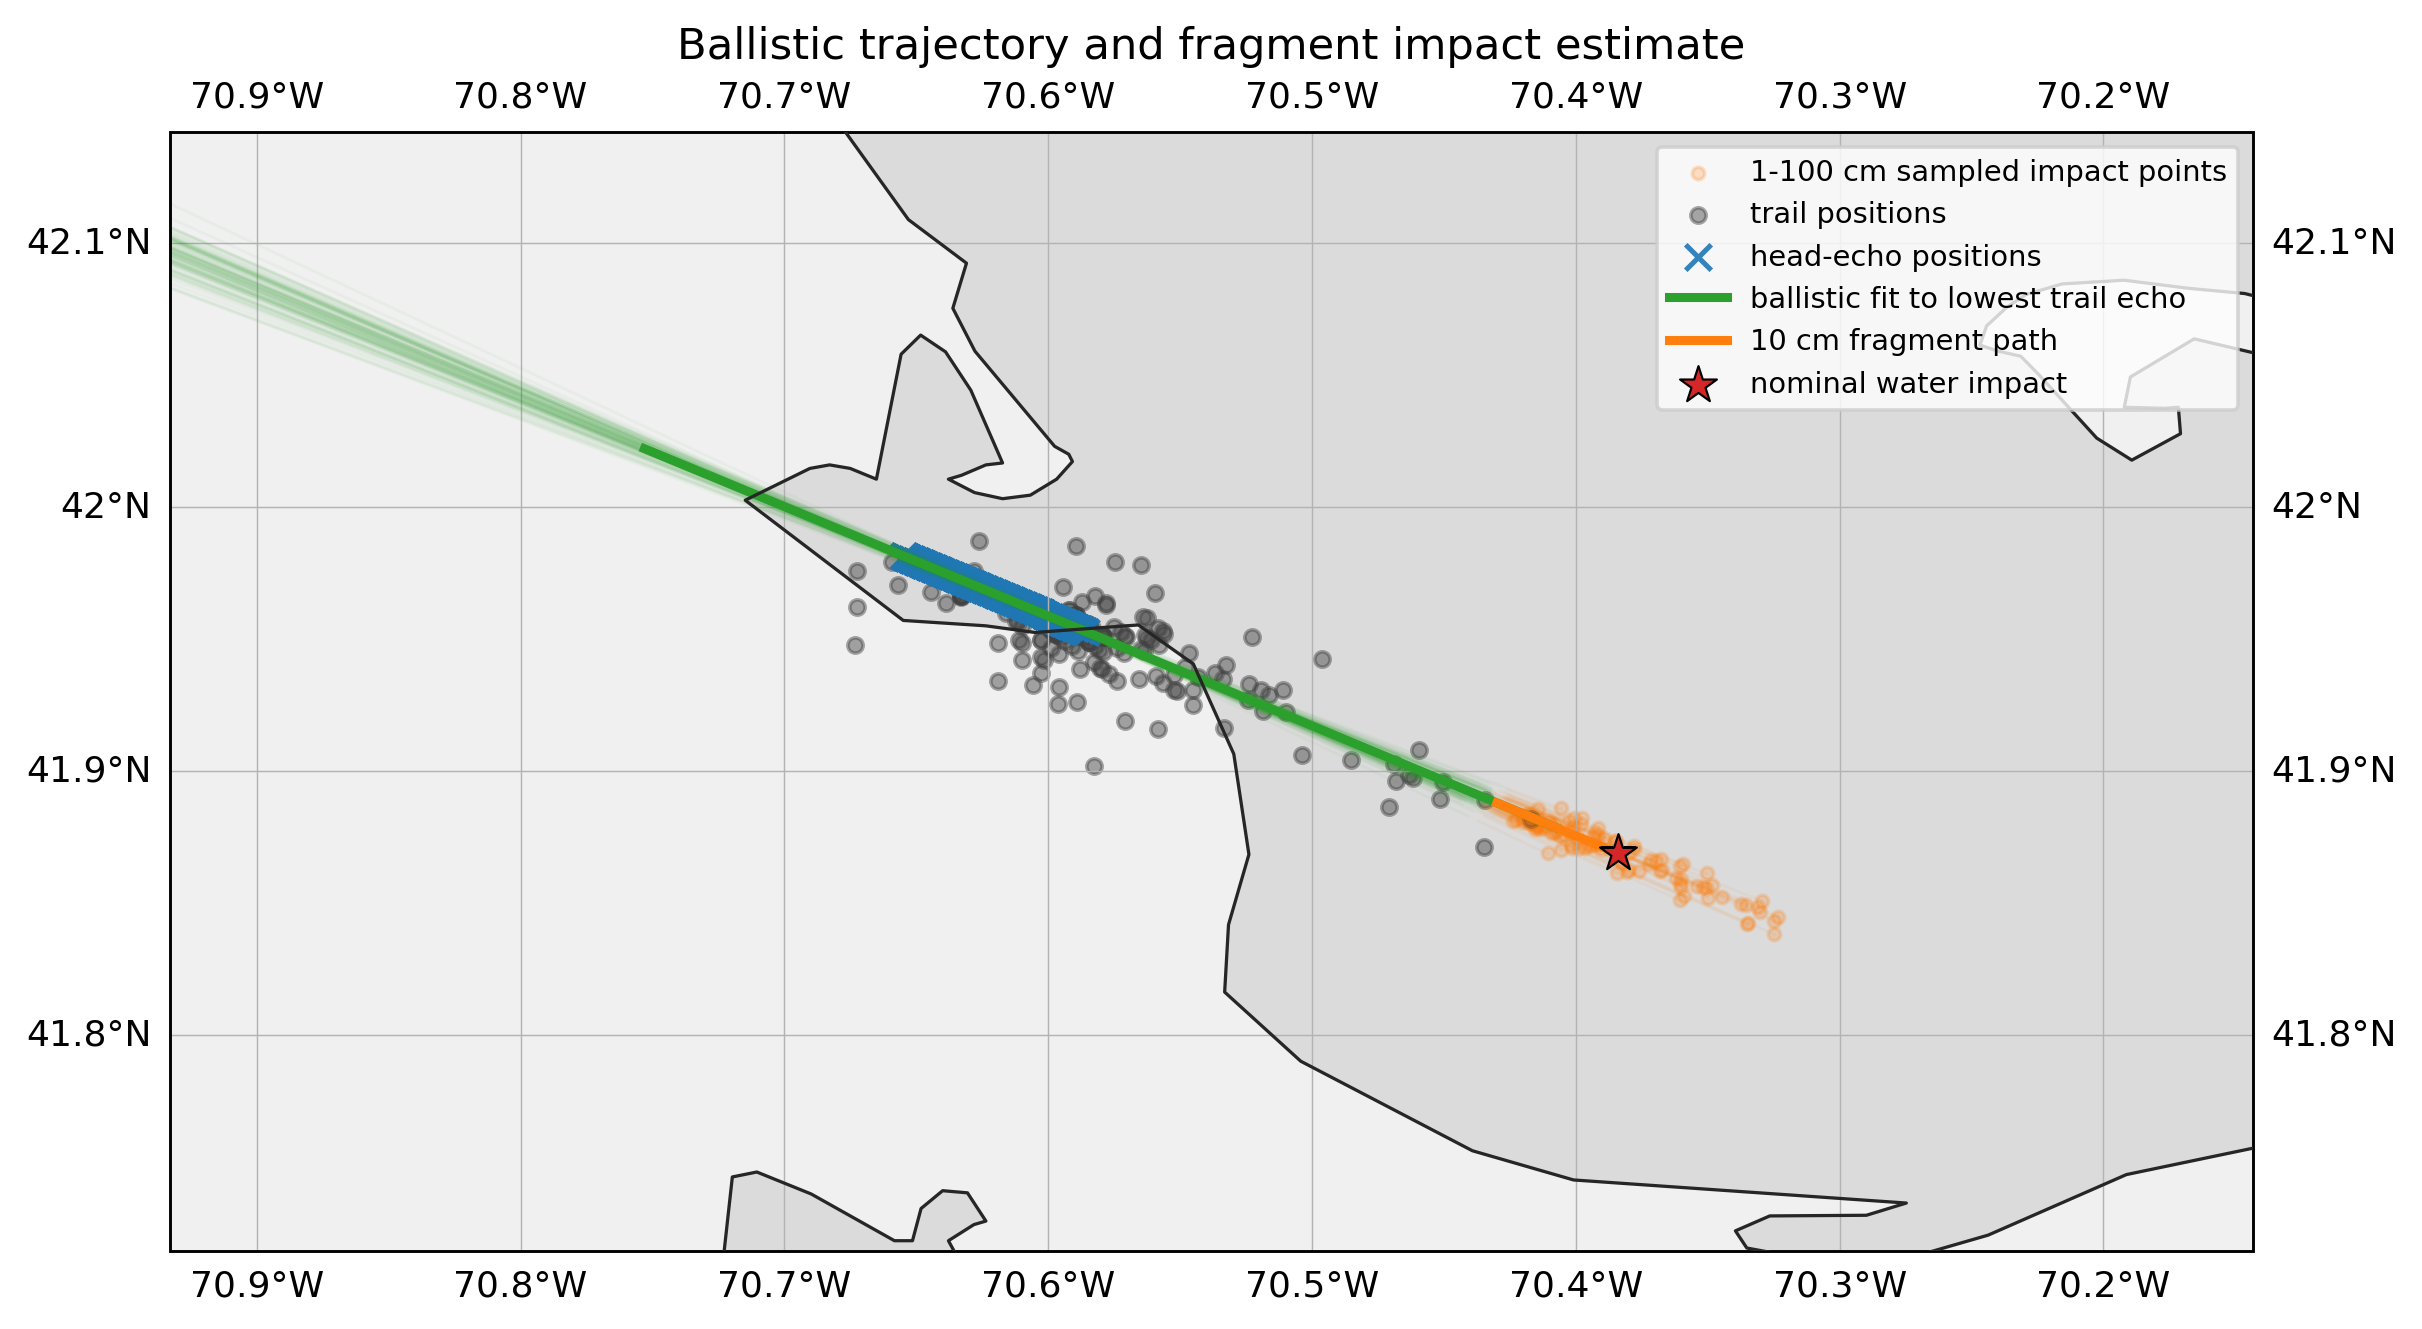
\includegraphics[width=\linewidth]{figures/ballistic_head_trail_impact_map.png}
  \caption{Ballistic trajectory and fragment-impact estimate.  The
  green curve shows the best-fit ballistic trajectory extended to the altitude
  of the lowest retained non-specular trail echo.  The orange curve is only the
  ground-fall extrapolation: below 30 km the object is assumed to have broken
  into 10 cm diameter spherical fragments of density
  \(3000\ \mathrm{kg\,m^{-3}}\), propagated with \(C_D=1\) so that
  \(C_D A/m = 0.005\ \mathrm{m^2\,kg^{-1}}\).  Orange points show sea-level
  impact samples obtained by varying the fragment diameter from 1 to 100 cm
  and sampling the ballistic-fit covariance.  The red star marks the nominal
  10 cm water-impact point in Cape Cod Bay.}
  \figsource{fit_ballistic_head_trail.py}
  \label{fig:ballistic-impact-map}
\end{figure}

\begin{table}[ht]
  \centering
  \caption{Sea-level impact estimate for the nominal 10 cm fragment and for fragment diameters sampled between 1 and 100 cm.  The sampled interval includes the linearized ballistic fit covariance and the unknown post-30 km fragment size at fixed density \(3000\ \mathrm{kg\,m^{-3}}\).}
  \label{tab:fragment-impact}
  \resizebox{\linewidth}{!}{%
  \begin{tabular}{lll}
    \toprule
    Quantity & Nominal 10 cm fragment & 95\% sampled interval \\
    \midrule
    Latitude (deg) & 41.8718 & 41.8747 [41.8480, 41.8878] \\
    Longitude (deg) & -70.3796 & -70.3895 [-70.4128, -70.3238] \\
    Sea-level time (UTC) & 18:11:18.9564 & 18:12:33.5408 [18:07:00.4247, 18:23:37.2135] \\
    Fall time below 30 km (s) & 296 & 371 [38, 1034] \\
    Impact speed (m s$^{-1}$) & 351 & 350 [347, 397] \\
    Fragment diameter (cm) & 10.0 & 7.0 [1.1, 85.3] \\
    \bottomrule
  \end{tabular}
  }
\end{table}


\begin{figure}[ht]
  \centering
  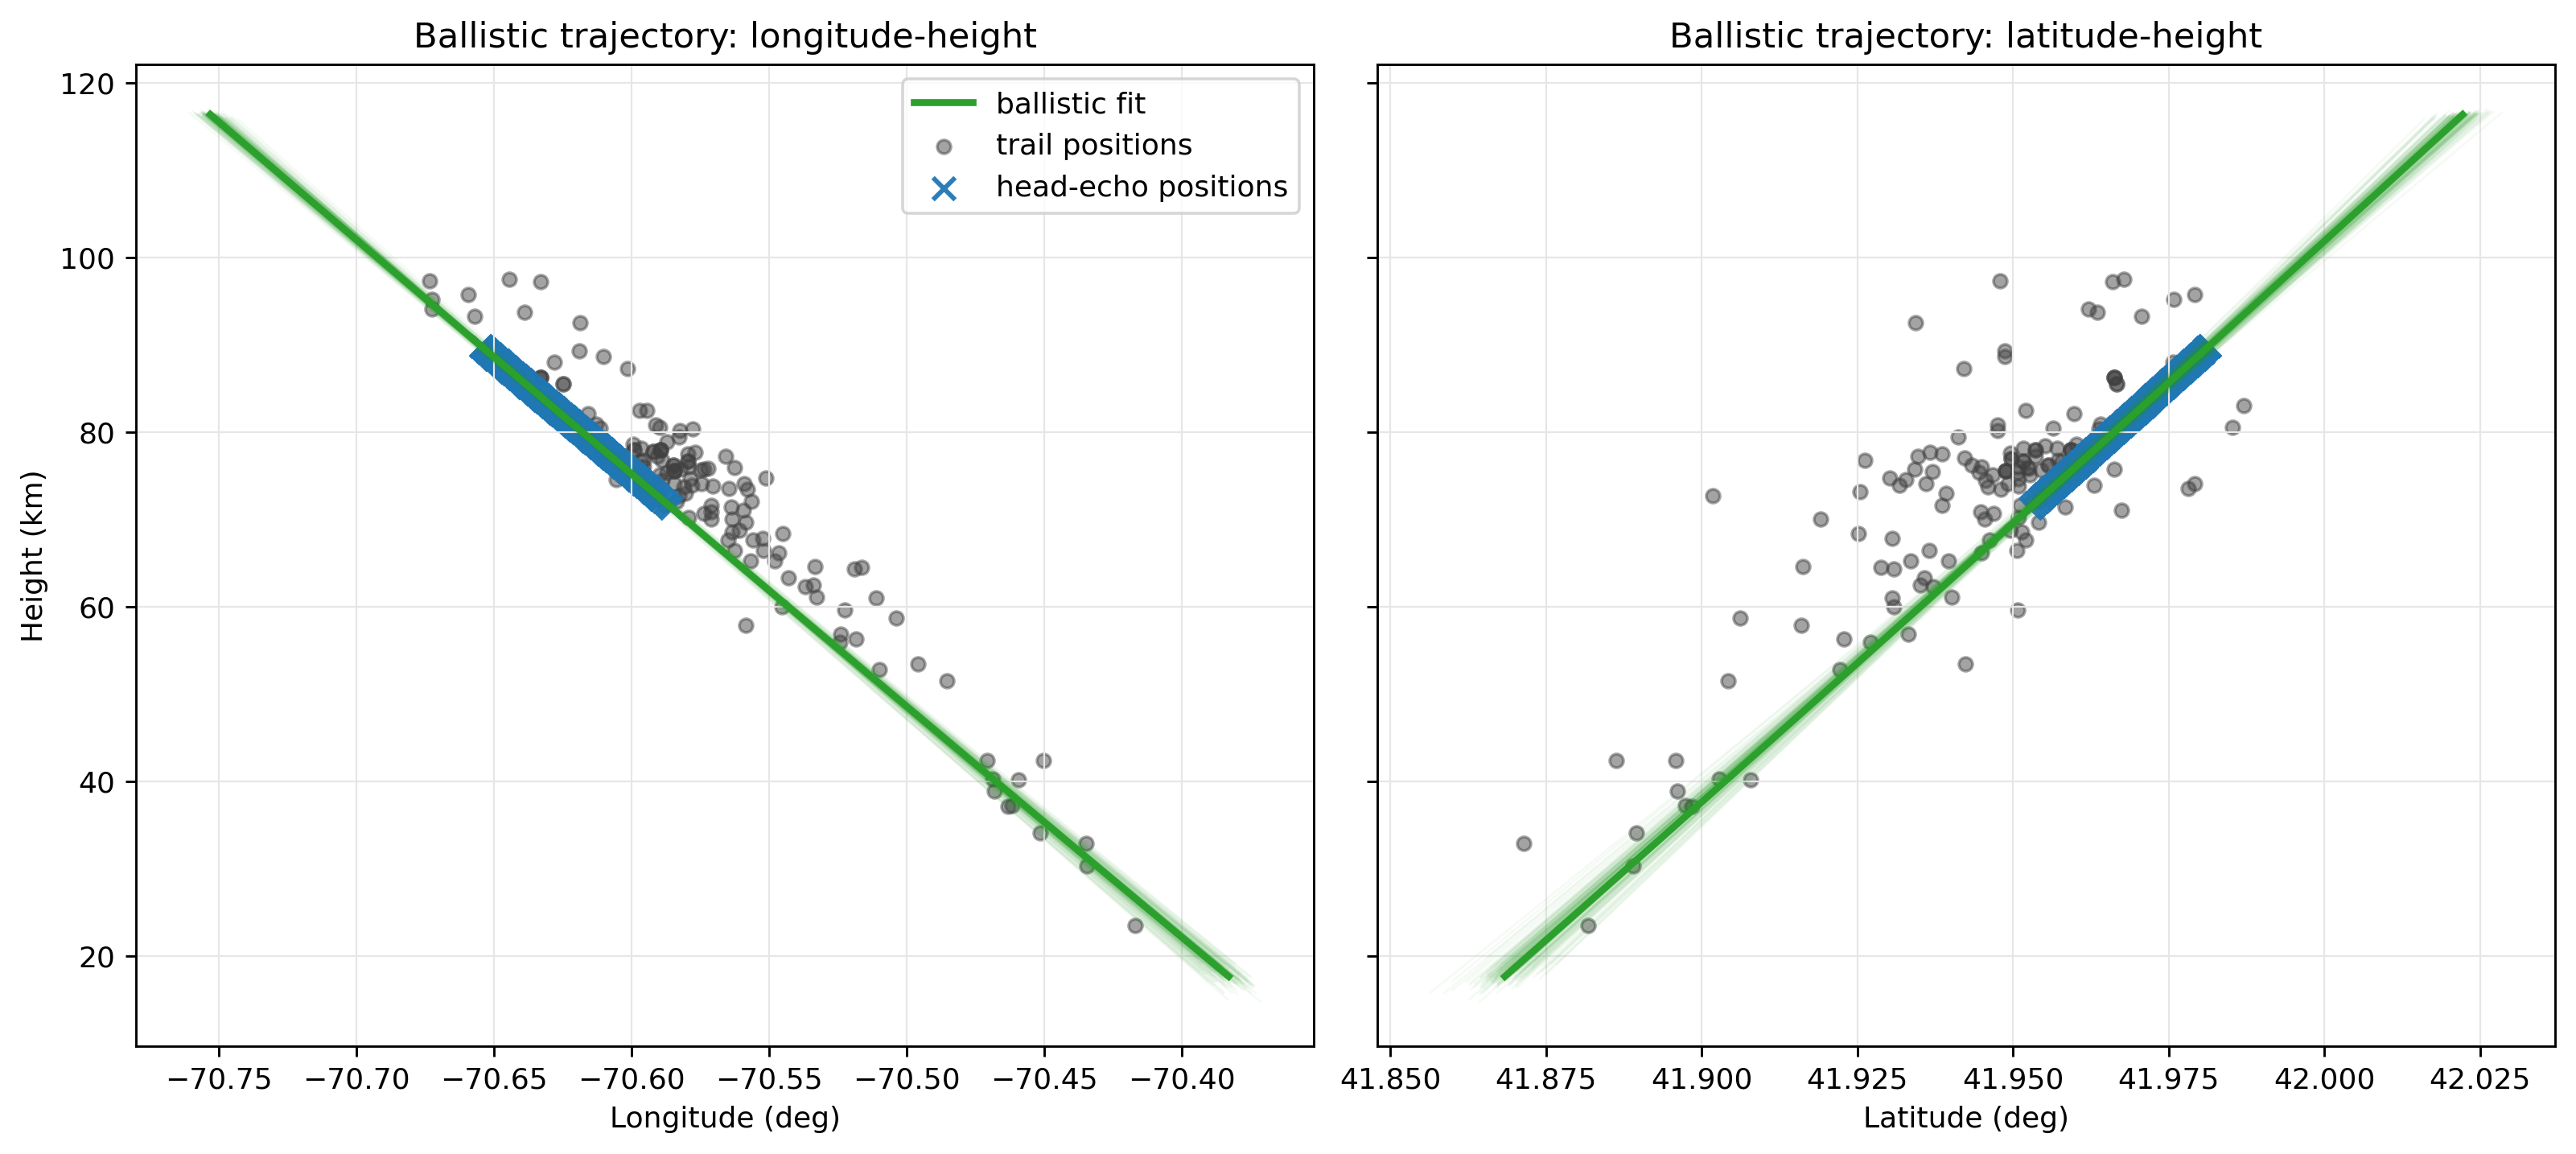
\includegraphics[width=\linewidth]{figures/ballistic_head_trail_lonlat_height.png}
  \caption{Ballistic head/trail trajectory fit shown as longitude versus height
  and latitude versus height.  The green curve is the best-fit trajectory under
  central gravity and fitted atmospheric drag; faint green curves are samples
  from the linearized fit covariance.  Gray points show retained non-specular
  trail positions, and blue crosses show head-echo-derived positions along the
  ballistic solution.}
  \figsource{fit_ballistic_head_trail.py}
  \label{fig:ballistic-lonlat-height}
\end{figure}

\begin{figure}[ht]
  \centering
  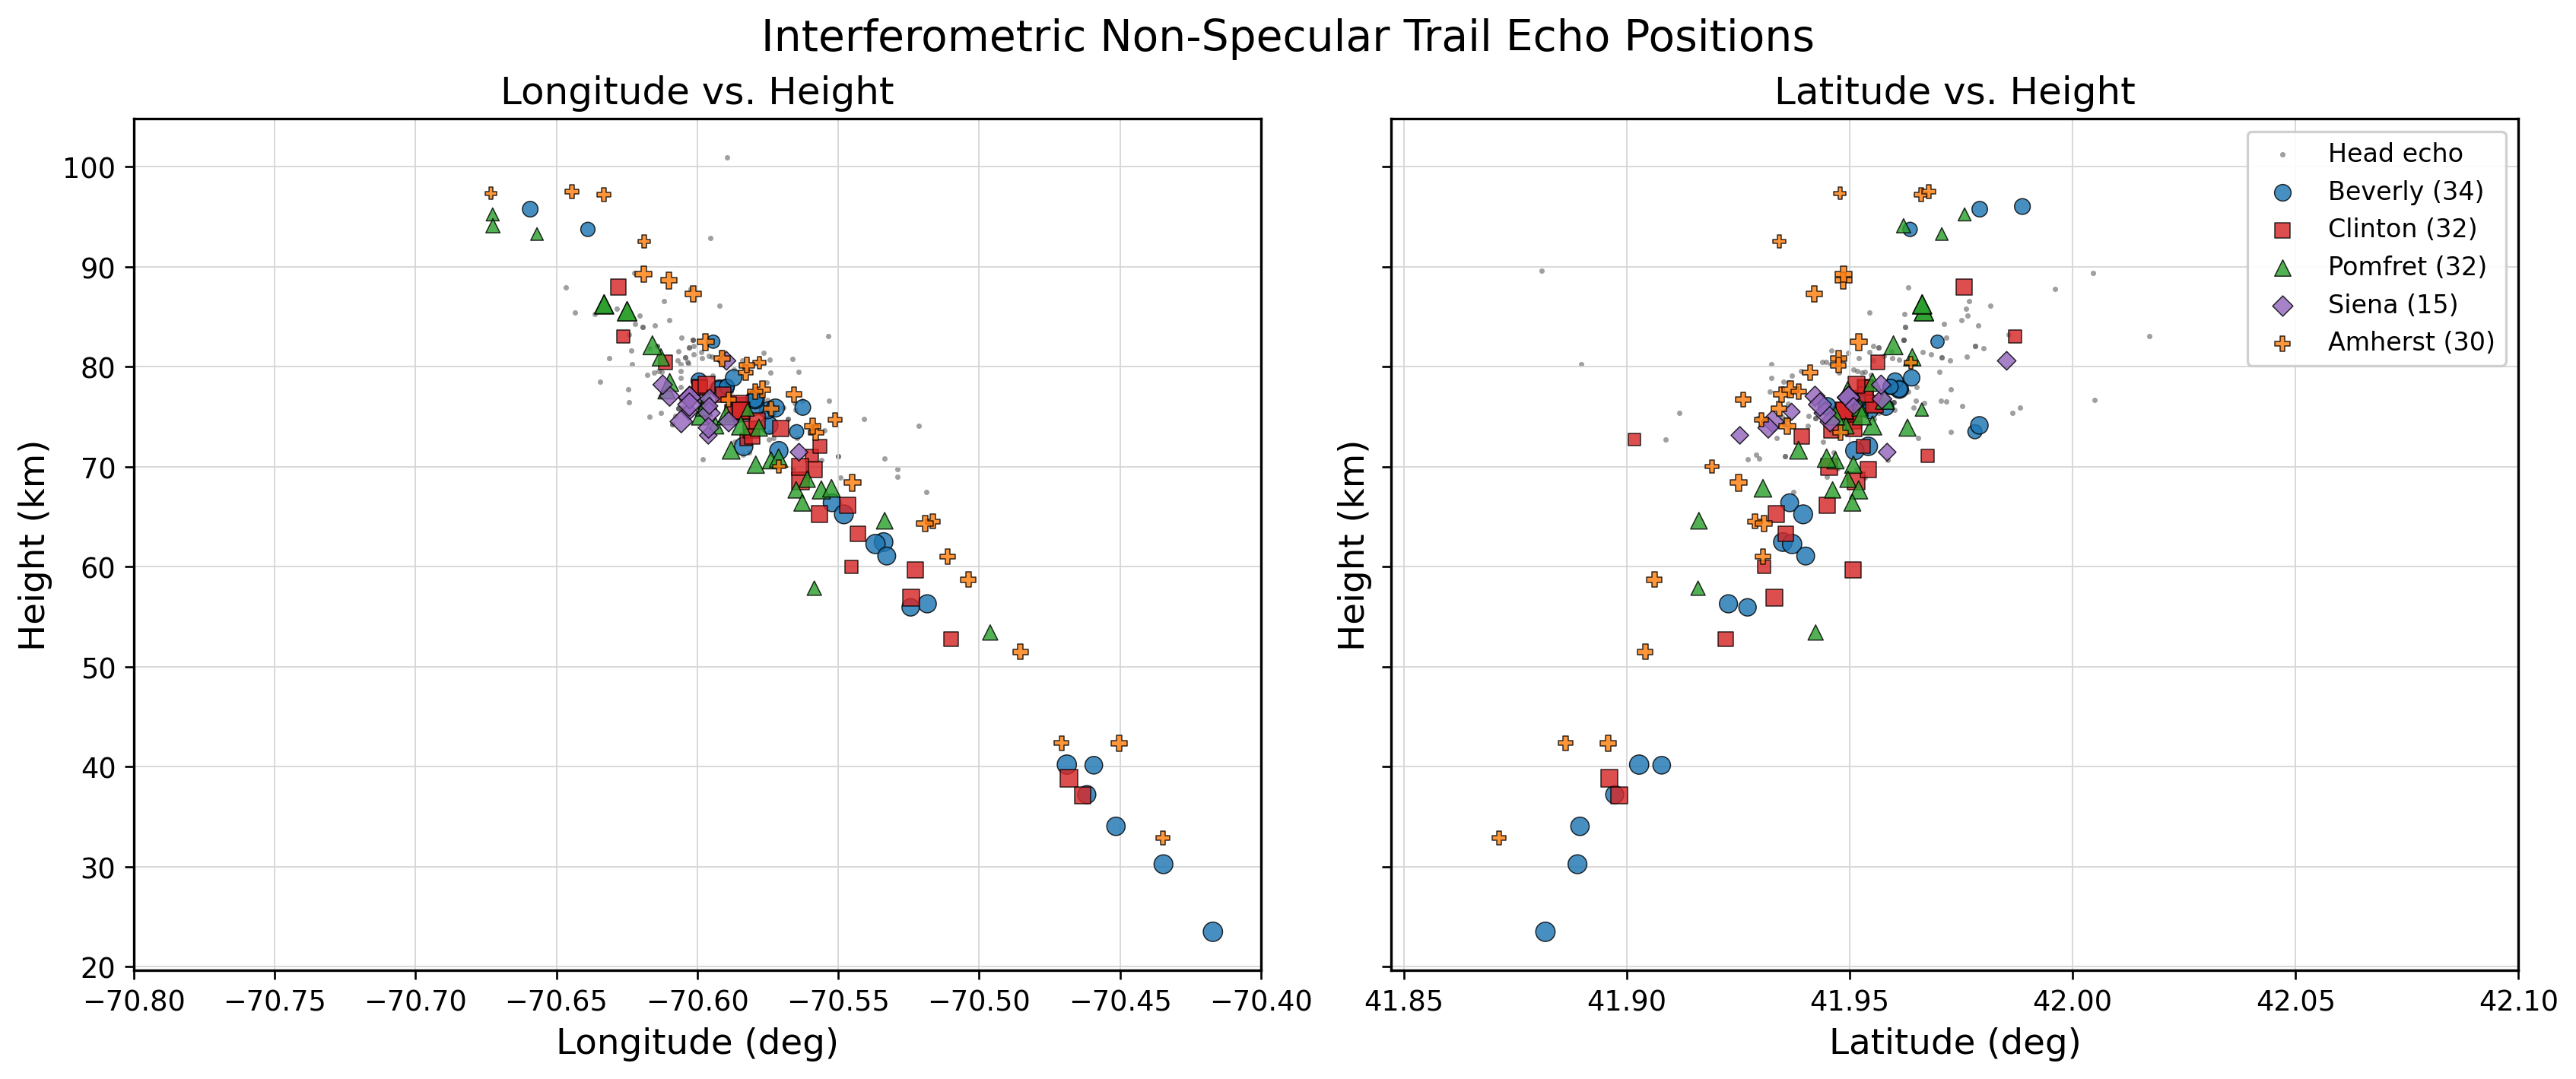
\includegraphics[width=\linewidth]{figures/trail_echo_geographic_height.png}
  \caption{Interferometric non-specular trail echo AoD plus bistatic-delay
  position solutions as a function of longitude and latitude versus height.
  Colors and marker shapes identify the receiving station used for the
  bistatic echo measurement; gray points show the corresponding head-echo AoD
  plus bistatic-delay positions.}
  \figsource{plot_interferometric_echo_geometry.py}
  \label{fig:trail-geographic-height}
\end{figure}

\begin{figure}[ht]
  \centering
  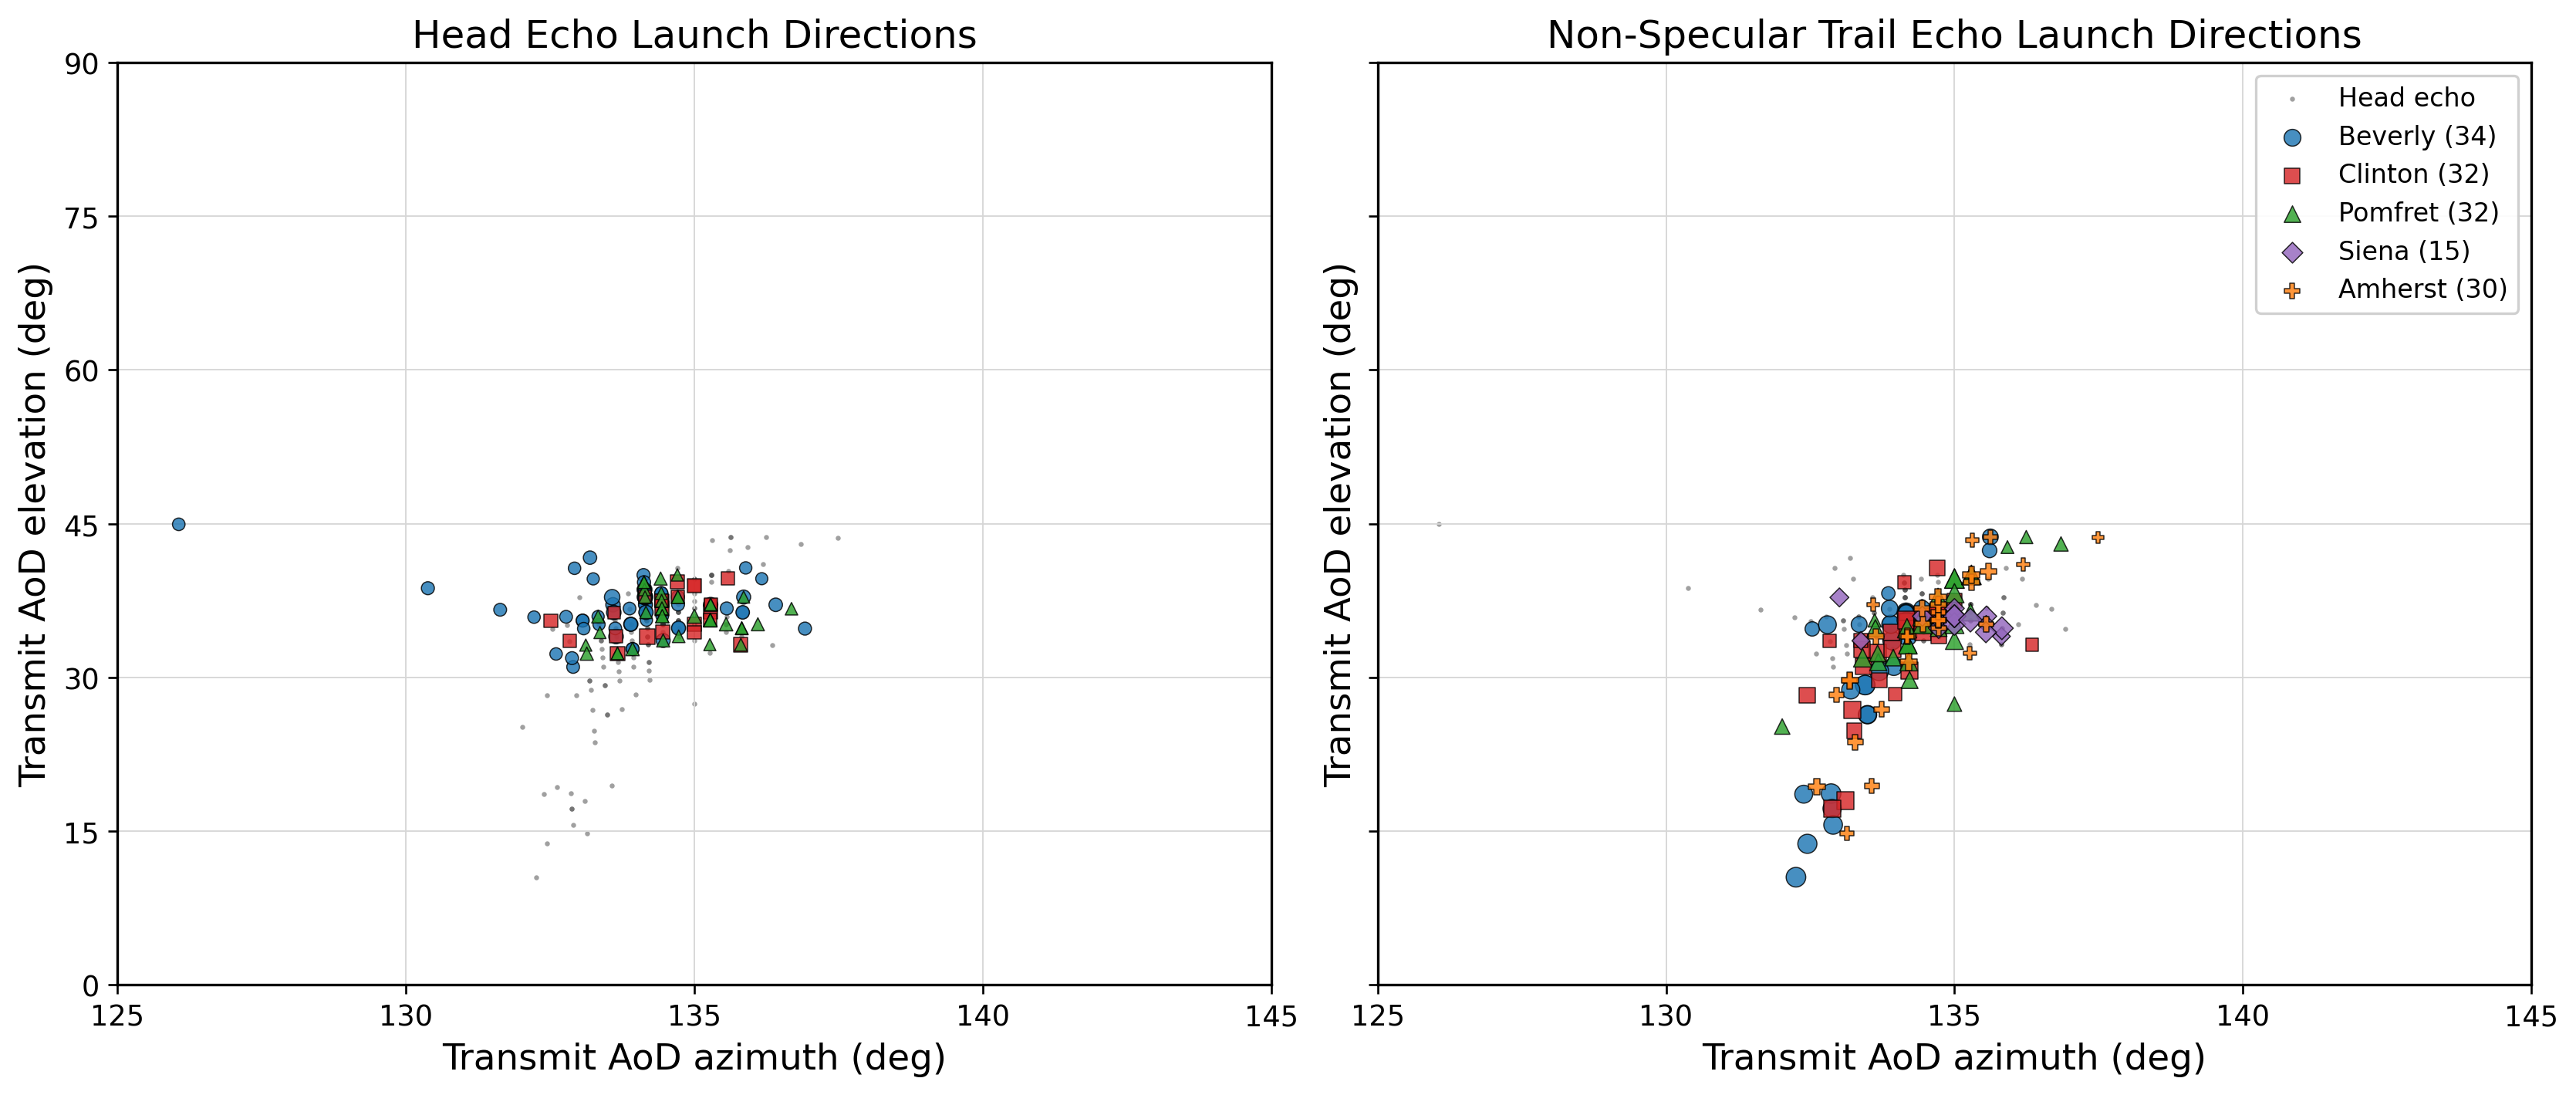
\includegraphics[width=\linewidth]{figures/head_trail_aod_launch_angles.png}
  \caption{Transmit angle-of-departure launch directions inferred by the
  five-antenna interferometer.  The left panel shows head-echo AoD solutions
  matched to the tri-static trajectory fit, and the right panel shows
  near-zero-Doppler non-specular trail echo AoD solutions.  Colors identify
  the receiving station.}
  \figsource{plot_interferometric_echo_geometry.py}
  \label{fig:head-trail-aod-launch}
\end{figure}

\section{Orbit and Source Association}

The heliocentric orbit was obtained by propagating the fitted radar
state backward with the JPL ephemeris until the object was outside
0.01 AU from Earth, then converting the resulting state to Keplerian elements
in the heliocentric mean ecliptic frame.  This orbit was compared with the
local MPC near-Earth asteroid catalogue in \texttt{data/NEA.txt}, the MPC
comet-element catalogue in \texttt{data/cometels.json.gz}, and the 2026 IAU Meteor
Data Center established shower list in
\texttt{data/streamestablisheddata2026.txt}.  The shower comparison uses only
established-shower entries whose reference field contains Jenniskens or Brown.
For comets and showers, the catalogue orbital elements are compared without
using a mean anomaly, because a comet/stream source comparison is based on
orbital-shape similarity rather than a single object at a specified orbital
phase.  The table therefore lists \(a,q,e,i,\omega,\Omega\), the catalogue
geocentric J2000 radiant RA/Dec where available, the Jopek \(D_H\) orbital
dissimilarity, and the angular radiant separation \(\Delta_R\).
The orbital uncertainties are obtained by drawing 200 states from
the empirically inflated \({\bf C}_{p}\), converting each sampled ENU state to
ECEF at the Haystack transmitter frame, and propagating each sample
independently.  Thus the trajectory covariance shown in
Figure~\ref{fig:trajectory-altitude}, including the residual-scatter
inflation, is also the source of the orbit-element, \(v_g\), and
corrected-radiant uncertainties in Table~\ref{tab:orbit-parameters} and
Figure~\ref{fig:orbit-xy}.

\begin{figure}[ht]
  \centering
  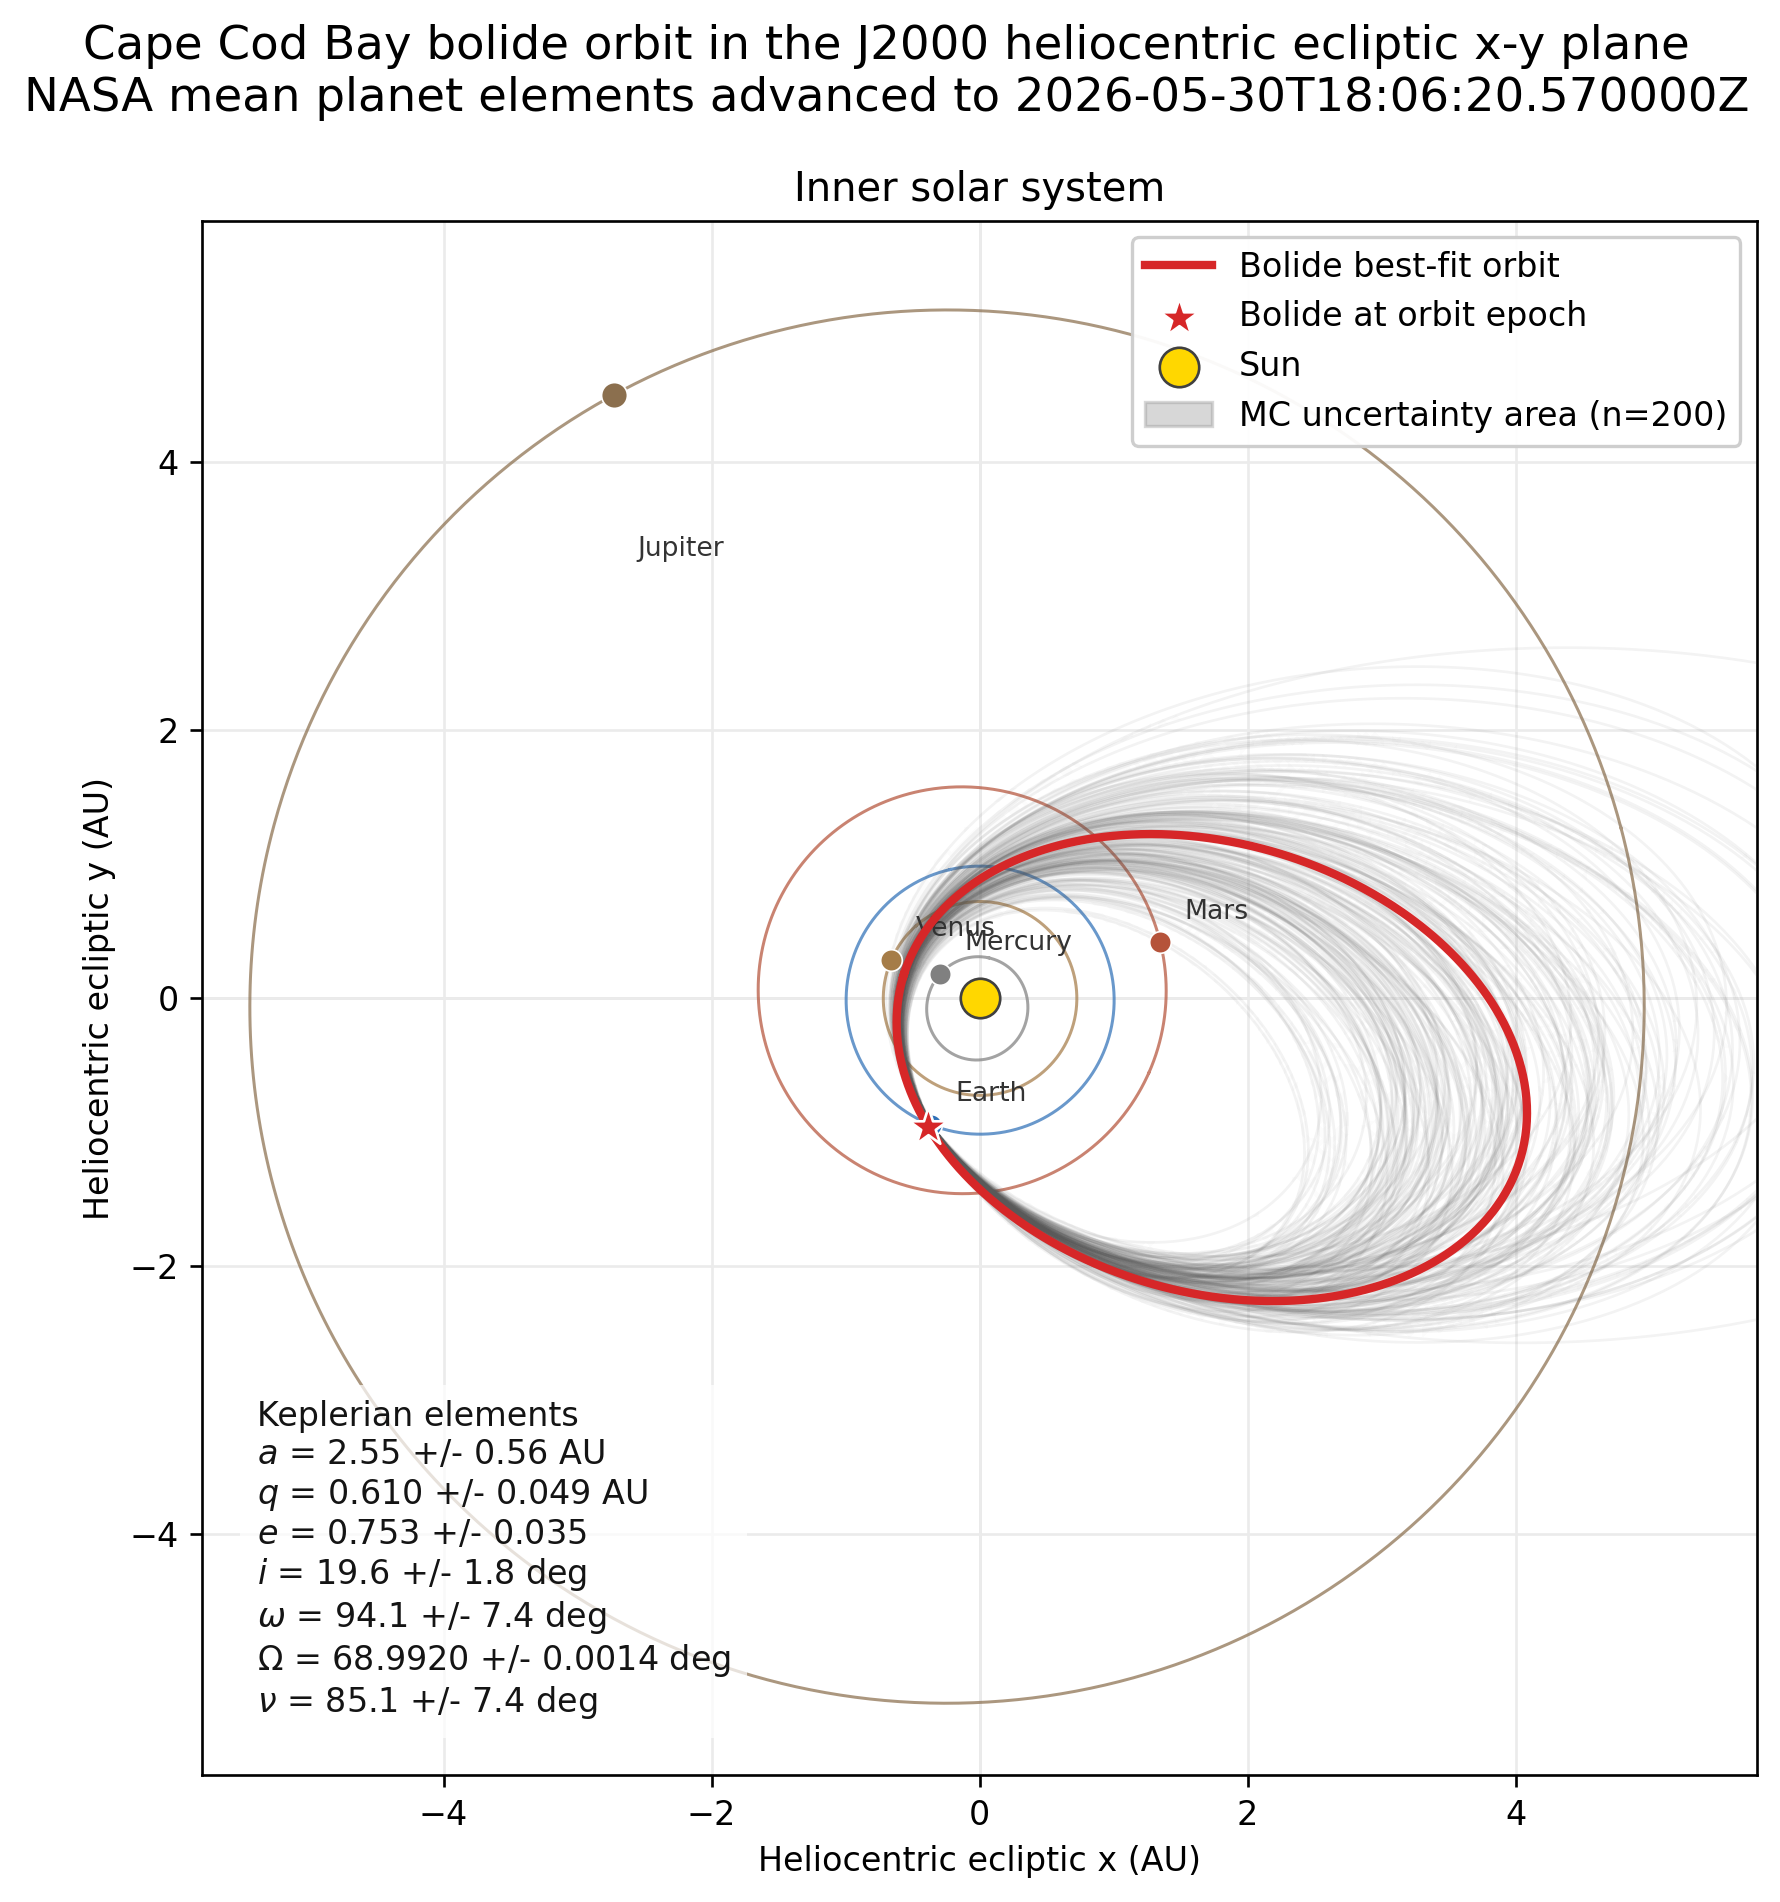
\includegraphics[width=\linewidth]{figures/orbit_xy_bolide.png}
  \caption{Best-fit bolide orbit in the J2000 heliocentric ecliptic \(x\)--\(y\)
  plane.  The plot zooms into the inner solar system and shows the Monte Carlo
  orbit uncertainty envelope from 200 trajectory-covariance samples with NASA
  mean planet elements advanced to the bolide epoch.}
  \figsource{plot_orbit_xy.py}
  \label{fig:orbit-xy}
\end{figure}

\begin{table}[ht]
  \centering
  \caption{Bolide heliocentric mean-ecliptic orbital elements and corrected
  geocentric speed and radiant with 1-sigma Monte Carlo uncertainties
  propagated from the six-parameter radar trajectory covariance.}
  \resizebox{0.78\linewidth}{!}{\begin{tabular}{llrl}
\toprule
Quantity & Symbol & Unit & Estimate \\
\midrule
Semimajor axis & $a$ & AU & 2.89 $\pm$ 0.07 \\
Perihelion distance & $q$ & AU & 0.628 $\pm$ 0.004 \\
Aphelion distance & $Q$ & AU & 5.16 $\pm$ 0.15 \\
Eccentricity & $e$ &  & 0.783 $\pm$ 0.005 \\
Inclination & $i$ & deg & 21.07 $\pm$ 0.17 \\
Argument of perihelion & $\omega$ & deg & 97.7 $\pm$ 0.6 \\
Longitude of ascending node & $\Omega$ & deg & 68.99081 $\pm$ 0.00011 \\
True anomaly at epoch & $\nu$ & deg & 81.6 $\pm$ 0.6 \\
Geocentric speed & $v_g$ & km s$^{-1}$ & 24.61 $\pm$ 0.11 \\
Tisserand parameter with respect to Jupiter & $T_J$ &  & 2.67 $\pm$ 0.04 \\
Corrected radiant right ascension & RA & deg & 59.88 $\pm$ 0.25 \\
Corrected radiant declination & Dec & deg & 48.56 $\pm$ 0.29 \\
Radiant azimuth at 100 km & Az & deg & 299.2 $\pm$ 0.9 \\
Radiant zenith angle at 100 km & $z$ & deg & 19.57 $\pm$ 0.13 \\
Geodetic latitude at 100 km & $\phi_{100}$ & deg & 41.9997 $\pm$ 0.0013 \\
Geodetic longitude at 100 km & $\lambda_{100}$ & deg & -70.6847 $\pm$ 0.0016 \\
Time at 100 km & $t_{100}$ & UTC & 2026-05-30 18:06:19.848 UTC $\pm$ 0.006 s \\
\bottomrule
\end{tabular}
}
  \label{tab:orbit-parameters}
\end{table}

\begin{table}[ht]
  \centering
  \caption{Best-fit bolide orbit and the closest catalogue matches.  The NEA
  entries are ranked from \texttt{data/NEA.txt}; comet entries are ranked from
  \texttt{data/cometels.json.gz}; stream entries are ranked from the established
  meteor stream catalogue.}
  \resizebox{\linewidth}{!}{% trajectory_fit_version: 0.2.1
% trajectory_fit_version_description: Selected head-echo correlated ballistic fit with mutual correlations within head-echo and trail-echo measurements. Head-echo correlations follow coherent-integration overlap in time; trail-position correlations require temporal overlap and the same raw range gate, with different range gates treated as uncorrelated.
\begin{tabular}{lrrrrrrrrrrl}
\toprule
Object/source & $a$ & $q$ & $e$ & $i$ & $\omega$ & $\Omega$ & RA & Dec & $D_H$ & $\Delta_R$ & Type \\
 & (AU) & (AU) & & (deg) & (deg) & (deg) & (deg) & (deg) & & (deg) & \\
\midrule
Bolide orbit sample mean & 3.266 & 0.645 & 0.794 & 18.42 & 100.15 & 68.99 & 63.95 & 46.75 & -- & -- &  \\
\midrule
2013 XG17 & 2.543 & 0.669 & 0.737 & 14.21 & 82.58 & 75.70 & -- & -- & 0.111 & -- & NEA \\
2024 XR16 & 2.454 & 0.574 & 0.766 & 18.69 & 106.34 & 74.98 & -- & -- & 0.120 & -- & NEA \\
2019 XH & 2.322 & 0.585 & 0.748 & 12.89 & 113.42 & 64.73 & -- & -- & 0.147 & -- & NEA \\
2001 WH1 & 2.478 & 0.508 & 0.795 & 15.60 & 108.62 & 67.02 & -- & -- & 0.175 & -- & NEA \\
1979 XB & 2.216 & 0.643 & 0.710 & 24.55 & 77.08 & 84.35 & -- & -- & 0.175 & -- & NEA \\
\midrule
P/2009 WX51 (Catalina) & 3.083 & 0.802 & 0.740 & 9.60 & 118.31 & 31.50 & -- & -- & 0.271 & -- & comet \\
209P/LINEAR & 2.957 & 0.963 & 0.674 & 21.29 & 152.48 & 62.74 & -- & -- & 0.372 & -- & comet \\
182P/LONEOS & 2.948 & 0.990 & 0.664 & 16.23 & 54.25 & 72.43 & -- & -- & 0.387 & -- & comet \\
364P/PANSTARRS & 2.905 & 0.827 & 0.715 & 11.81 & 213.01 & 45.60 & -- & -- & 0.445 & -- & comet \\
P/2013 CU129 (PANSTARRS) & 2.905 & 0.827 & 0.715 & 11.81 & 213.01 & 45.60 & -- & -- & 0.445 & -- & comet \\
\midrule
OER omicron-Eridanids                        & 3.910 & 0.513 & 0.865 & 20.20 & 92.70 & 48.10 & 56.1 & -2.2 & 0.248 & 49.4 & stream \\
OER omicron-Eridanids                        & 3.920 & 0.497 & 0.875 & 19.60 & 94.10 & 49.20 & 59.9 & 0.1 & 0.252 & 46.8 & stream \\
ORS Southern chi-Orionids                    & 2.170 & 0.398 & 0.817 & 5.10 & 109.00 & 69.30 & 78.4 & 17.9 & 0.367 & 31.2 & stream \\
ORS Southern chi-Orionids                    & 2.160 & 0.381 & 0.828 & 5.30 & 111.30 & 64.30 & 73.0 & 17.8 & 0.378 & 29.9 & stream \\
SCC Southern delta-Cancrids                  & 2.230 & 0.411 & 0.816 & 4.90 & 107.20 & 100.90 & 112.2 & 17.1 & 0.405 & 49.4 & stream \\
SCC Southern delta-Cancrids                  & 2.260 & 0.430 & 0.811 & 4.70 & 105.00 & 109.30 & 125.0 & 14.4 & 0.412 & 59.8 & stream \\
\bottomrule
\end{tabular}
}
  \label{tab:orbit-source}
\end{table}

The radar-derived radiant used for the stream comparison is the
zenithal-attraction-corrected radiant from the orbit solution, not the apparent
local radiant shown in Figure~\ref{fig:trajectory-altitude}.  This corrected
radiant was estimated directly from the sampled orbital solutions and is shown
with its 95\% uncertainty region in Figure~\ref{fig:shower-radiants}.  Shower
marker area scales with the number of meteors \(N\) listed in the established
shower catalogue, so large markers indicate better-populated shower solutions
rather than larger angular uncertainty.

\begin{figure}[ht]
  \centering
  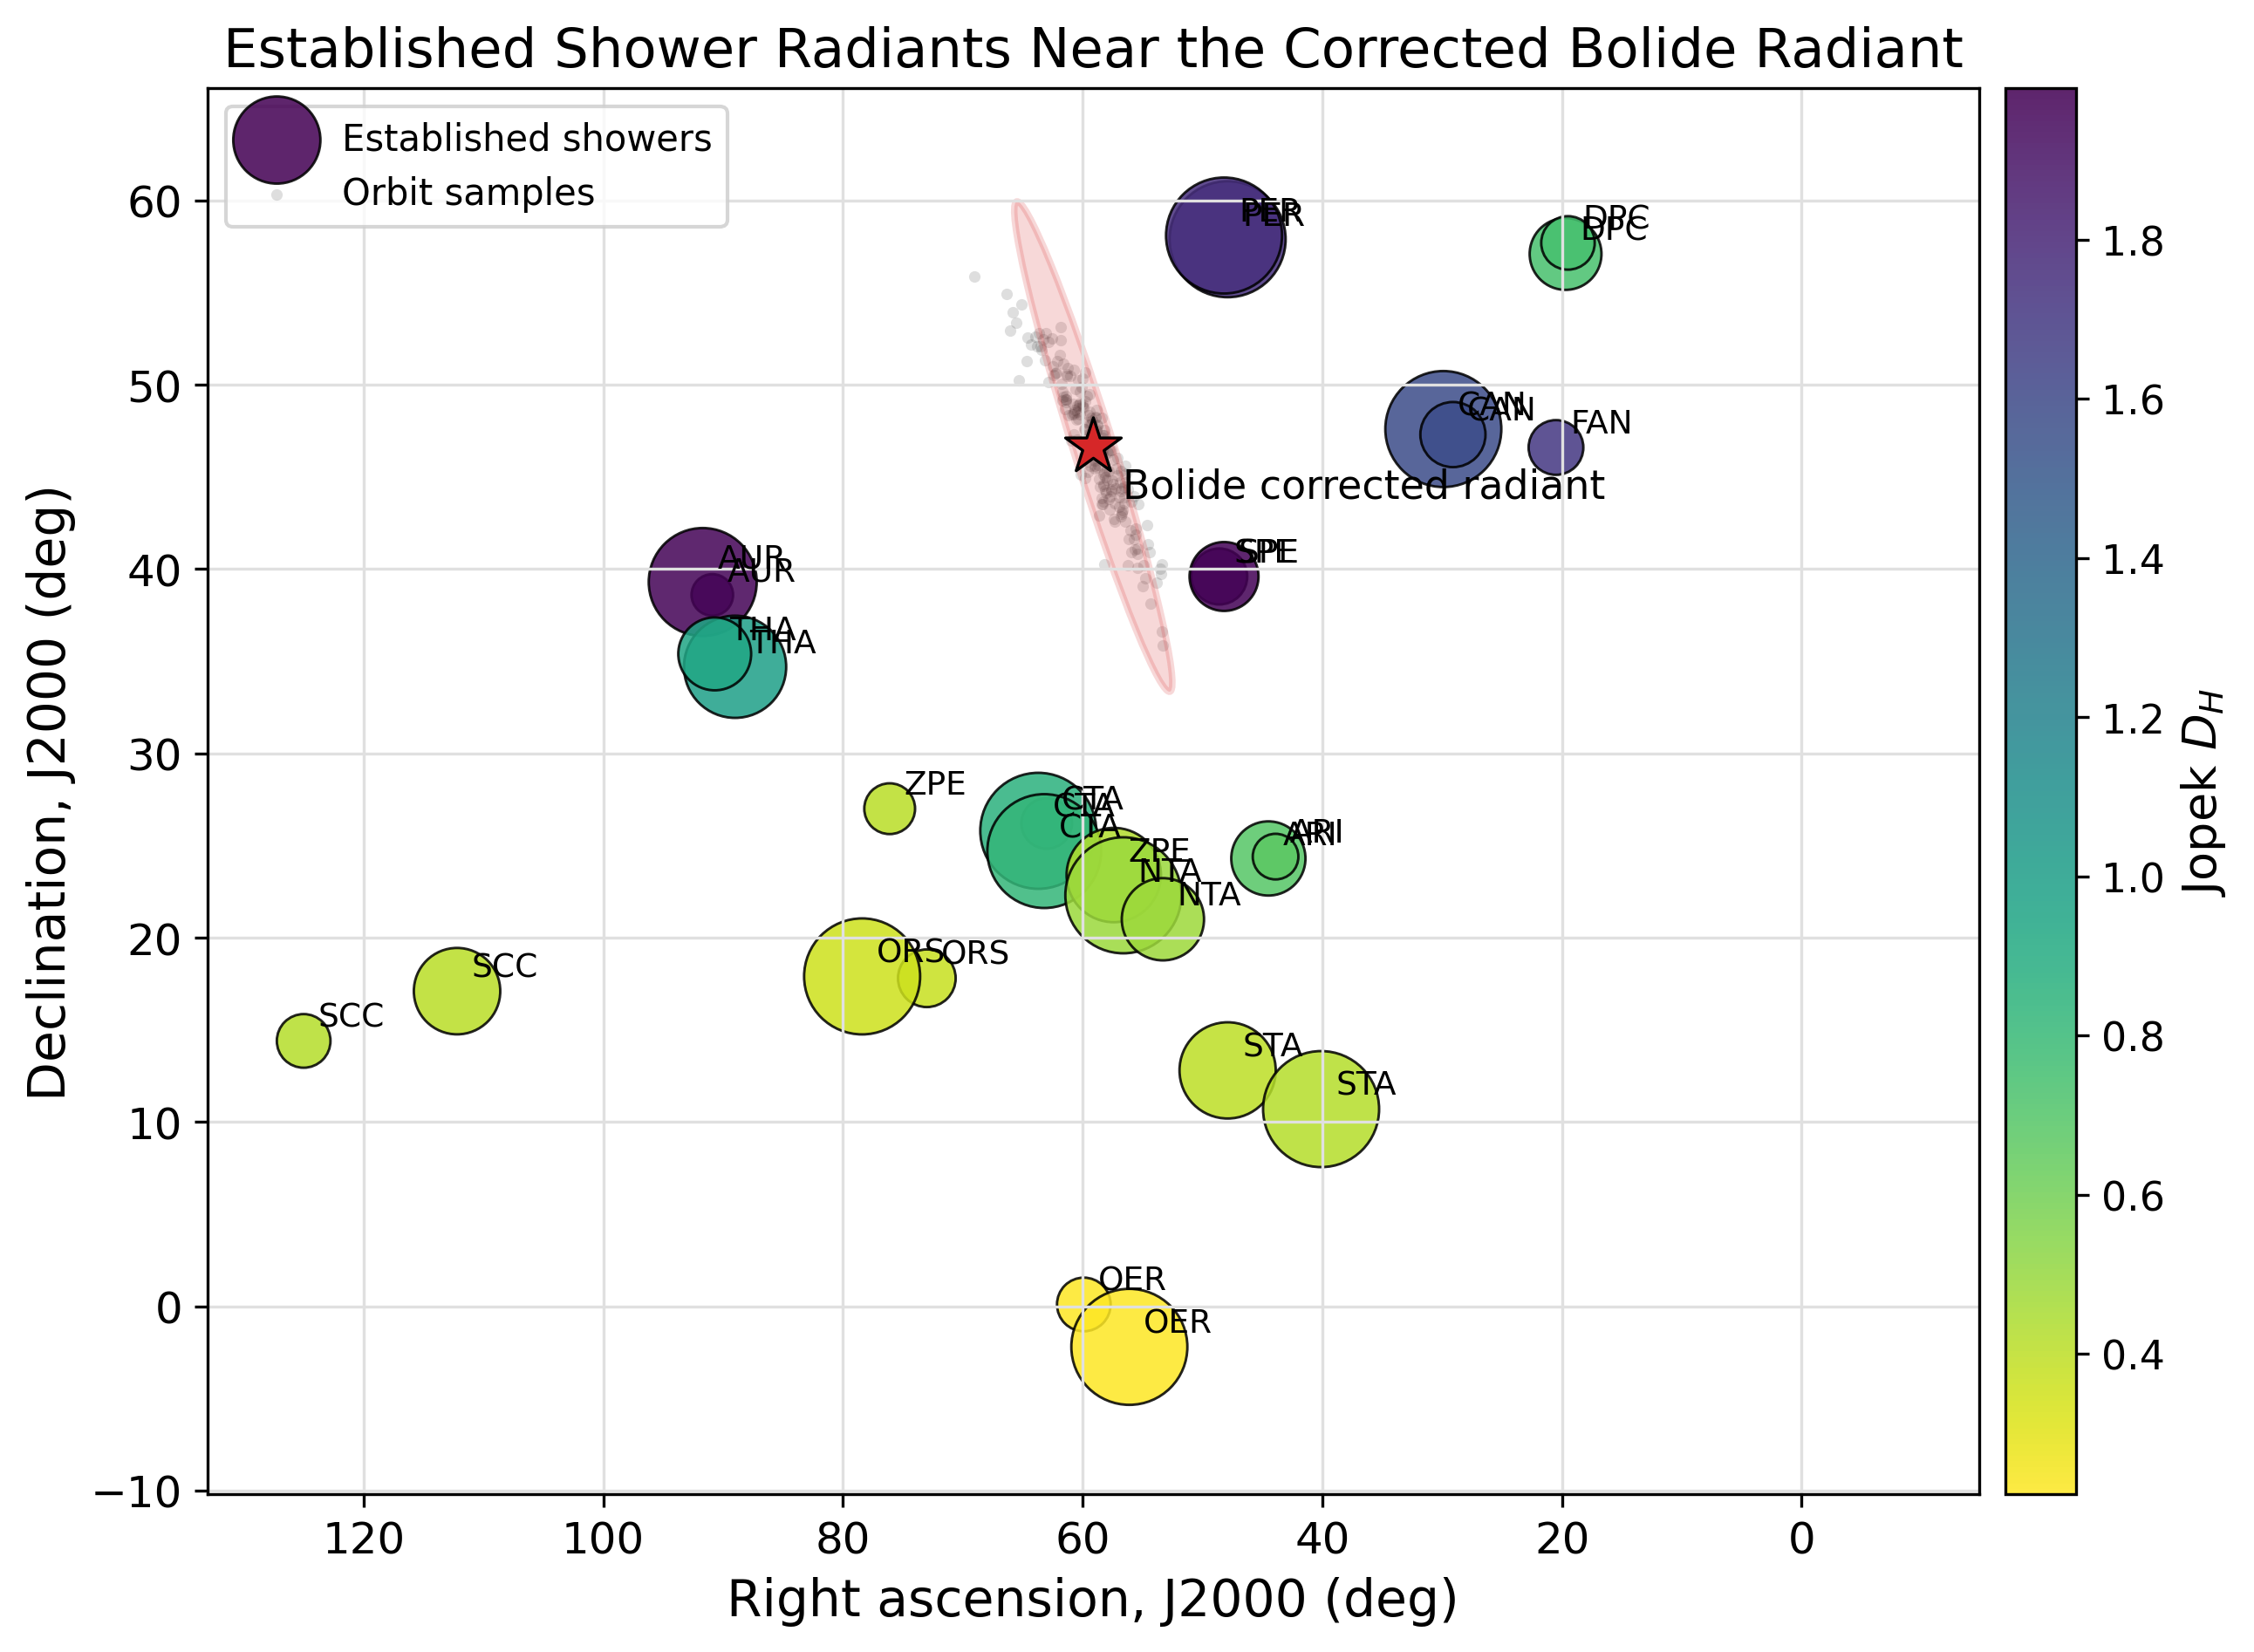
\includegraphics[width=0.92\linewidth]{figures/shower_radiant_comparison.png}
  \caption{Corrected bolide radiant compared with nearby established shower
  radiants from Jenniskens or Brown catalogue entries.  The bolide marker and
  shaded ellipse show the mean and sampled 95\% zenithal-attraction-corrected
  radiant uncertainty.  Shower marker area scales with catalogue member count,
  and color gives Jopek \(D_H\) orbital dissimilarity.}
  \figsource{plot_shower_radiants.py}
  \label{fig:shower-radiants}
\end{figure}

The closest NEA, comet, and established-shower entries are listed in
Table~\ref{tab:orbit-source}.  Agreement in \(D_H\) alone is not sufficient for
source identification: the radiant RA/Dec and geocentric speed provide
additional constraints, and the closest orbital-element match can still be a
poor radiant match.  Conversely, a nearby radiant without orbital-element
agreement is not by itself evidence for association.

The similar-body search should therefore be read as an orbital-neighbour
search rather than a parent-body identification.  The \(D_H\) function is a
hybrid form of the classical Southworth--Hawkins orbital dissimilarity
criterion \cite{southworth_hawkins_1963,jopek_1993}, and recent reviews
emphasize that \(D\)-criteria identify orbital similarity rather than genetic
association by themselves \cite{courtot_shober_vaubaillon_2026}.  Previous
radar stream tests also show that a single cutoff is not universal but depends
on the orbit distribution, inclination regime, measurement uncertainty, and
sporadic background \cite{galligan_2001,courtot_shober_vaubaillon_2026}.  In
the present catalogue comparison,
\(D_H \leq 0.15\) is used only as a practical flag for notable orbital
neighbours.  By this criterion the search finds several NEAs with similar
orbits, including 2024 XR16 with \(D_H=0.099\), but no comparable comet match:
the closest comet is P/2009 WX51 (Catalina) with \(D_H=0.300\).  No
established shower is similar.  The closest shower by \(D_H\), the
omicron-Eridanids, has \(D_H=0.224\) and a corrected-radiant separation of
about \(48^\circ\), making it a poor association despite being the nearest
listed shower in orbital-element space.

\section{Discussion and Conclusions}

The radar observations provide complementary constraints on the bolide.
Doppler-gated head echoes determine the line-of-flight and velocity, while
near-zero-Doppler non-specular trail echoes provide AoD plus bistatic-delay
position samples along the ionized trail.  The solution is internally
consistent across the range, Doppler, AoD, and coordinate-system products, and
the Monte Carlo orbit propagation gives the uncertainty envelope used for
source association.  The catalogue comparison is therefore best interpreted as
a ranked orbital and radiant similarity search rather than a unique
parent-body identification.

\appendix

\section{Instrument Geometry}
\label{app:instrument}

The receiving sites are identified by compact station labels.  The tables in
this appendix translate those labels to geographic receiver sites and list the
shared Haystack transmit site used by all bistatic paths.

\begin{table}[ht]
  \centering
  \caption{Transmit and receive station coordinates from the analysis
  configuration files.}
  \resizebox{\linewidth}{!}{\begin{tabular}{lrrrl}
\toprule
Place & Latitude (deg) & Longitude (deg) & Altitude (m) & Role \\
\midrule
Haystack, Massachusetts & 42.611495 & -71.484666 & 79.0 & transmitter \\
Beverly, Massachusetts & 42.551324 & -70.901134 & -8.2 & receiver \\
Clinton, Massachusetts & 42.419328 & -71.677843 & 91.8 & receiver \\
Pomfret, Vermont & 43.717156 & -72.434666 & 152.8 & receiver \\
Siena College, New York & 42.719476 & -73.752195 & 86.6 & receiver \\
Amherst, New Hampshire & 42.828043 & -71.573002 & 56.1 & receiver \\
\bottomrule
\end{tabular}
}
  \label{tab:station-coordinates}
\end{table}

The coded-CW transmitter used five transmit antennas.  Their local ENU offsets
are relative to the transmitter reference point in
Table~\ref{tab:station-coordinates}.  Each antenna is associated with one
pseudo-random transmit-code seed.

\begin{table}[ht]
  \centering
  \caption{Haystack transmit antenna offsets and pseudo-random code seeds.}
  \begin{tabular}{rrrr}
\toprule
TX index & East (m) & North (m) & Seed \\
\midrule
0 & -16.14 & -11.49 & 48 \\
1 & -17.30 & 11.89 & 915 \\
2 & 4.47 & 20.65 & 5976 \\
3 & 18.85 & 2.10 & 8952 \\
4 & 4.93 & -17.88 & 13898 \\
\bottomrule
\end{tabular}

  \label{tab:tx-antennas}
\end{table}

\begin{figure}[ht]
  \centering
  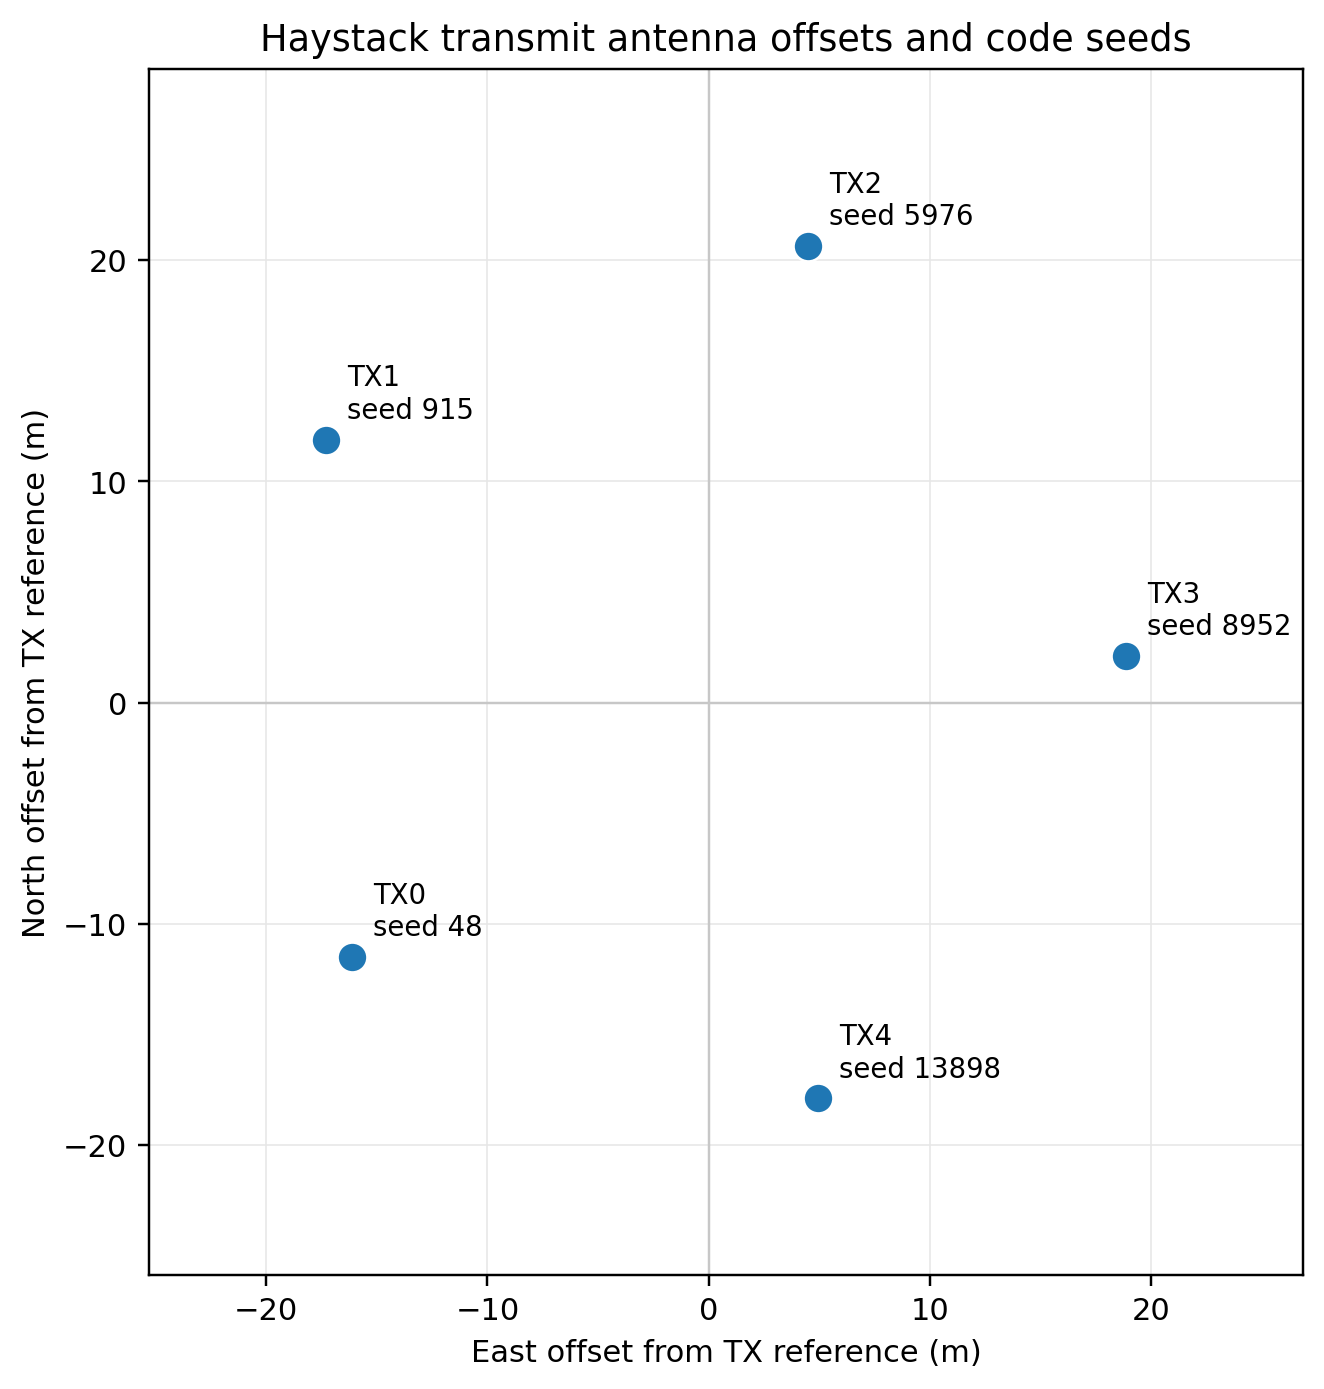
\includegraphics[width=0.72\linewidth]{figures/tx_antenna_coordinates.png}
  \caption{Transmit antenna ENU offsets and the corresponding code seeds.}
  \figsource{reports/generate_station_config_assets.py}
  \label{fig:tx-antennas}
\end{figure}

\begin{figure}[ht]
  \centering
  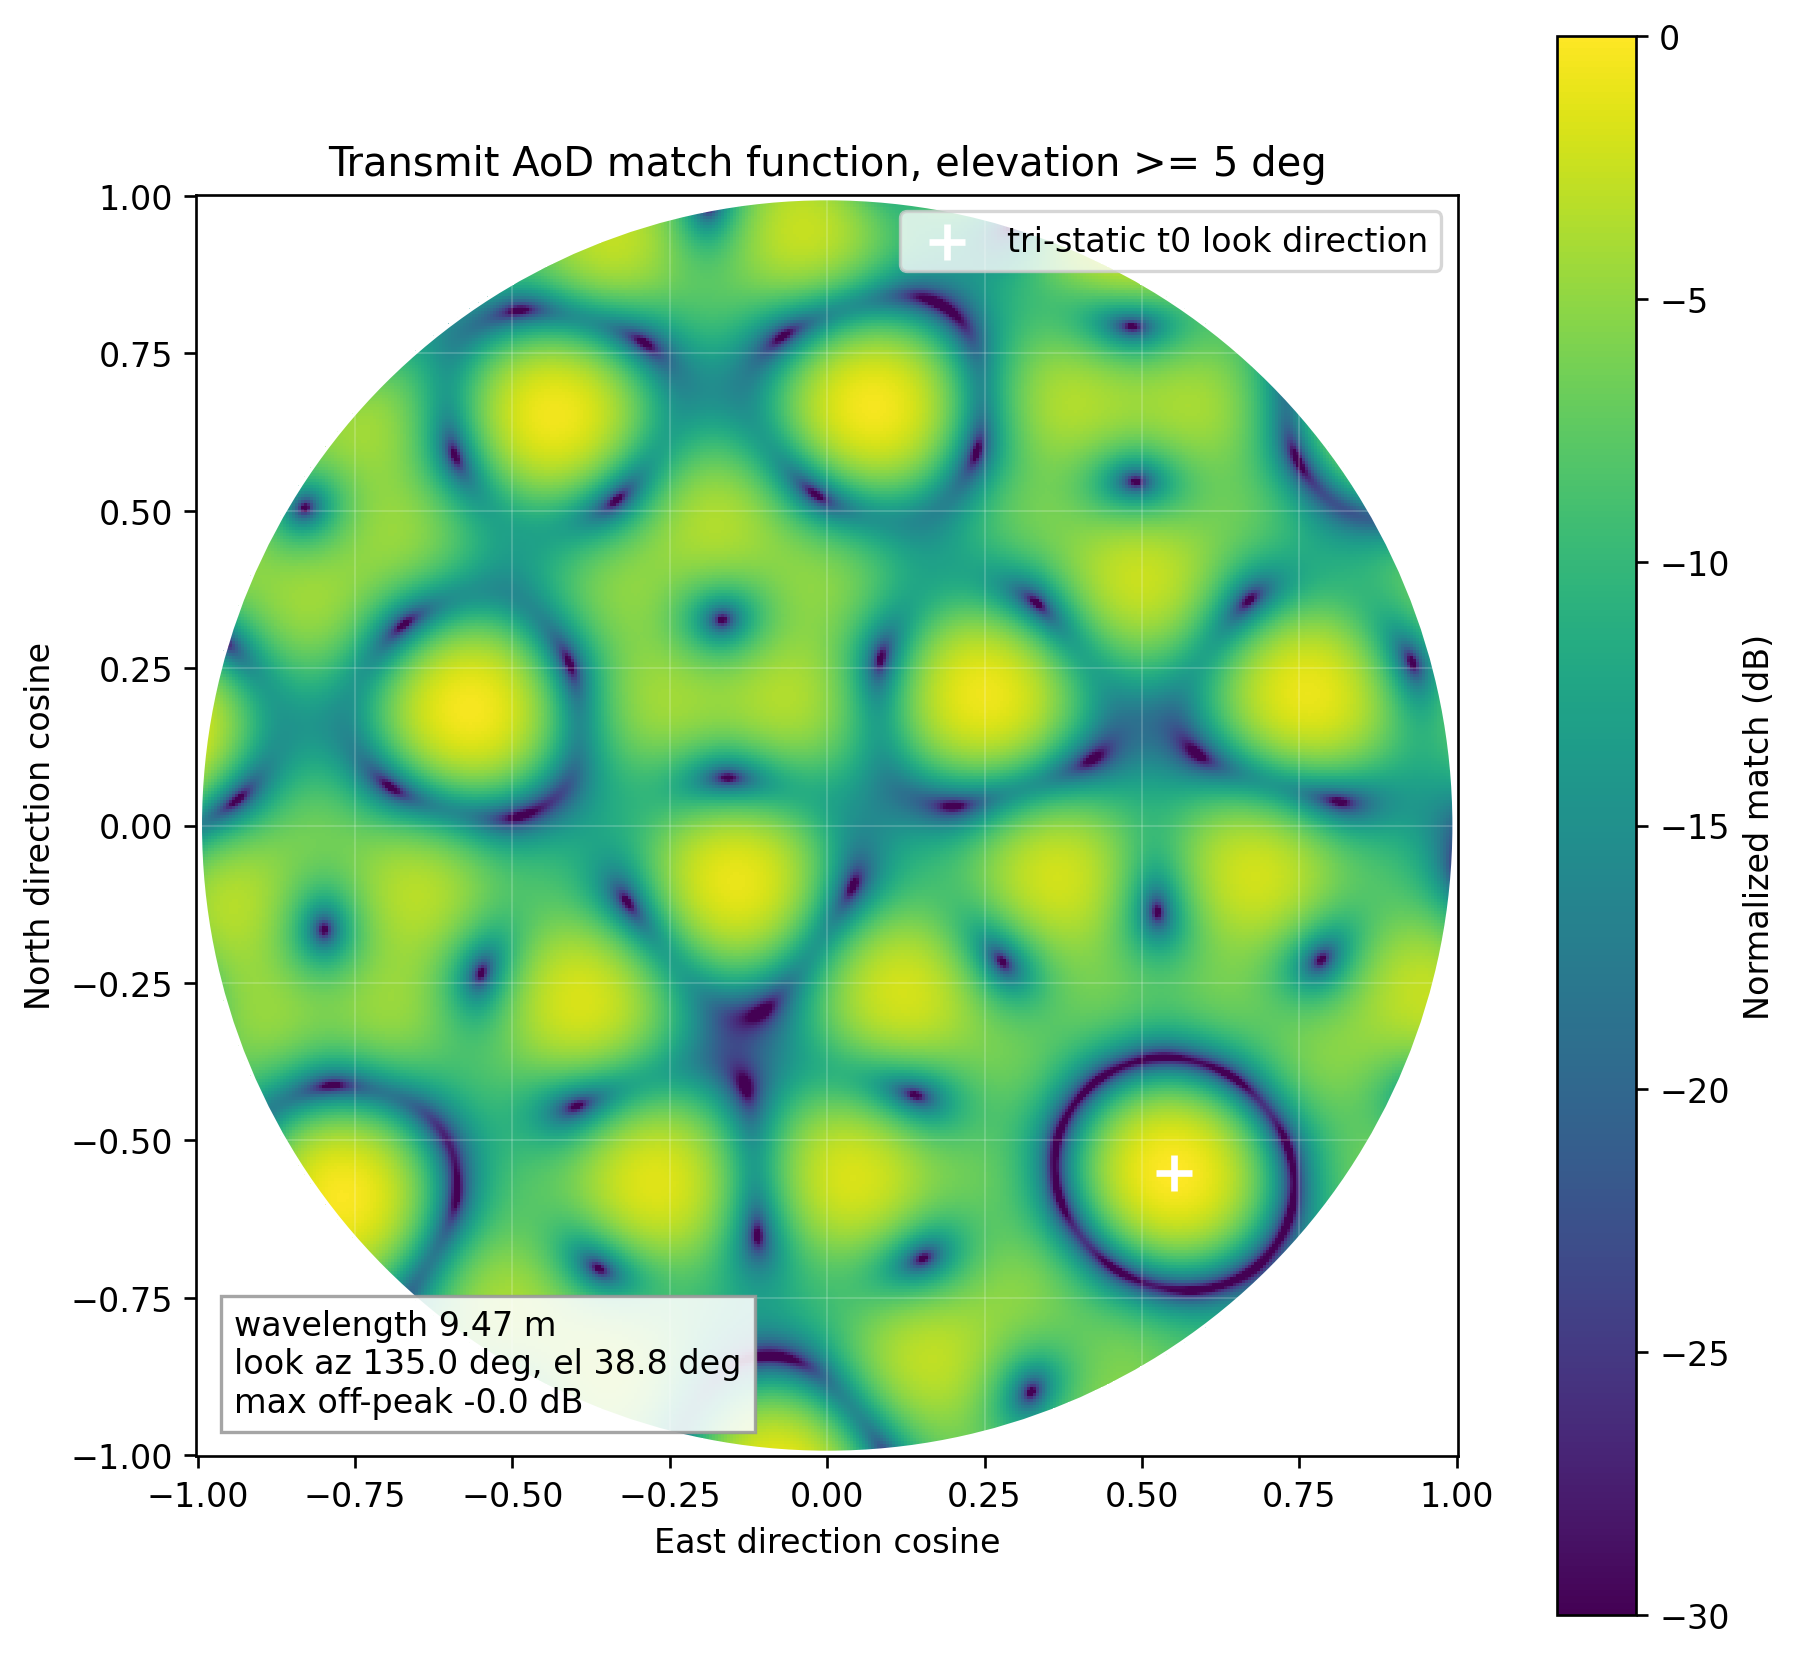
\includegraphics[width=0.78\linewidth]{figures/tx_aod_match_function.png}
  \caption{Normalized transmit-array angle-of-departure match function in
  east/north direction cosines for the a priori look direction implied by the
  tri-static head-echo fit at the reference time.  The sky is masked below
  5 deg elevation.  This shows the angular response and sidelobe/ambiguity
  structure expected from the five-antenna transmit interferometer before
  measurement noise and echo SNR are considered.}
  \figsource{reports/generate_station_config_assets.py}
  \label{fig:tx-aod-match}
\end{figure}

\section{Processing Diagnostics}
\label{app:processing-diagnostics}

The processing code supports optional robust impulsive-sample excision, but
this step was disabled for the high-resolution products used in the trajectory
and trail analysis.  The diagnostic in this section shows the samples that
would have been removed under the conservative spike-excision threshold used
for testing.

\begin{figure}[ht]
  \centering
  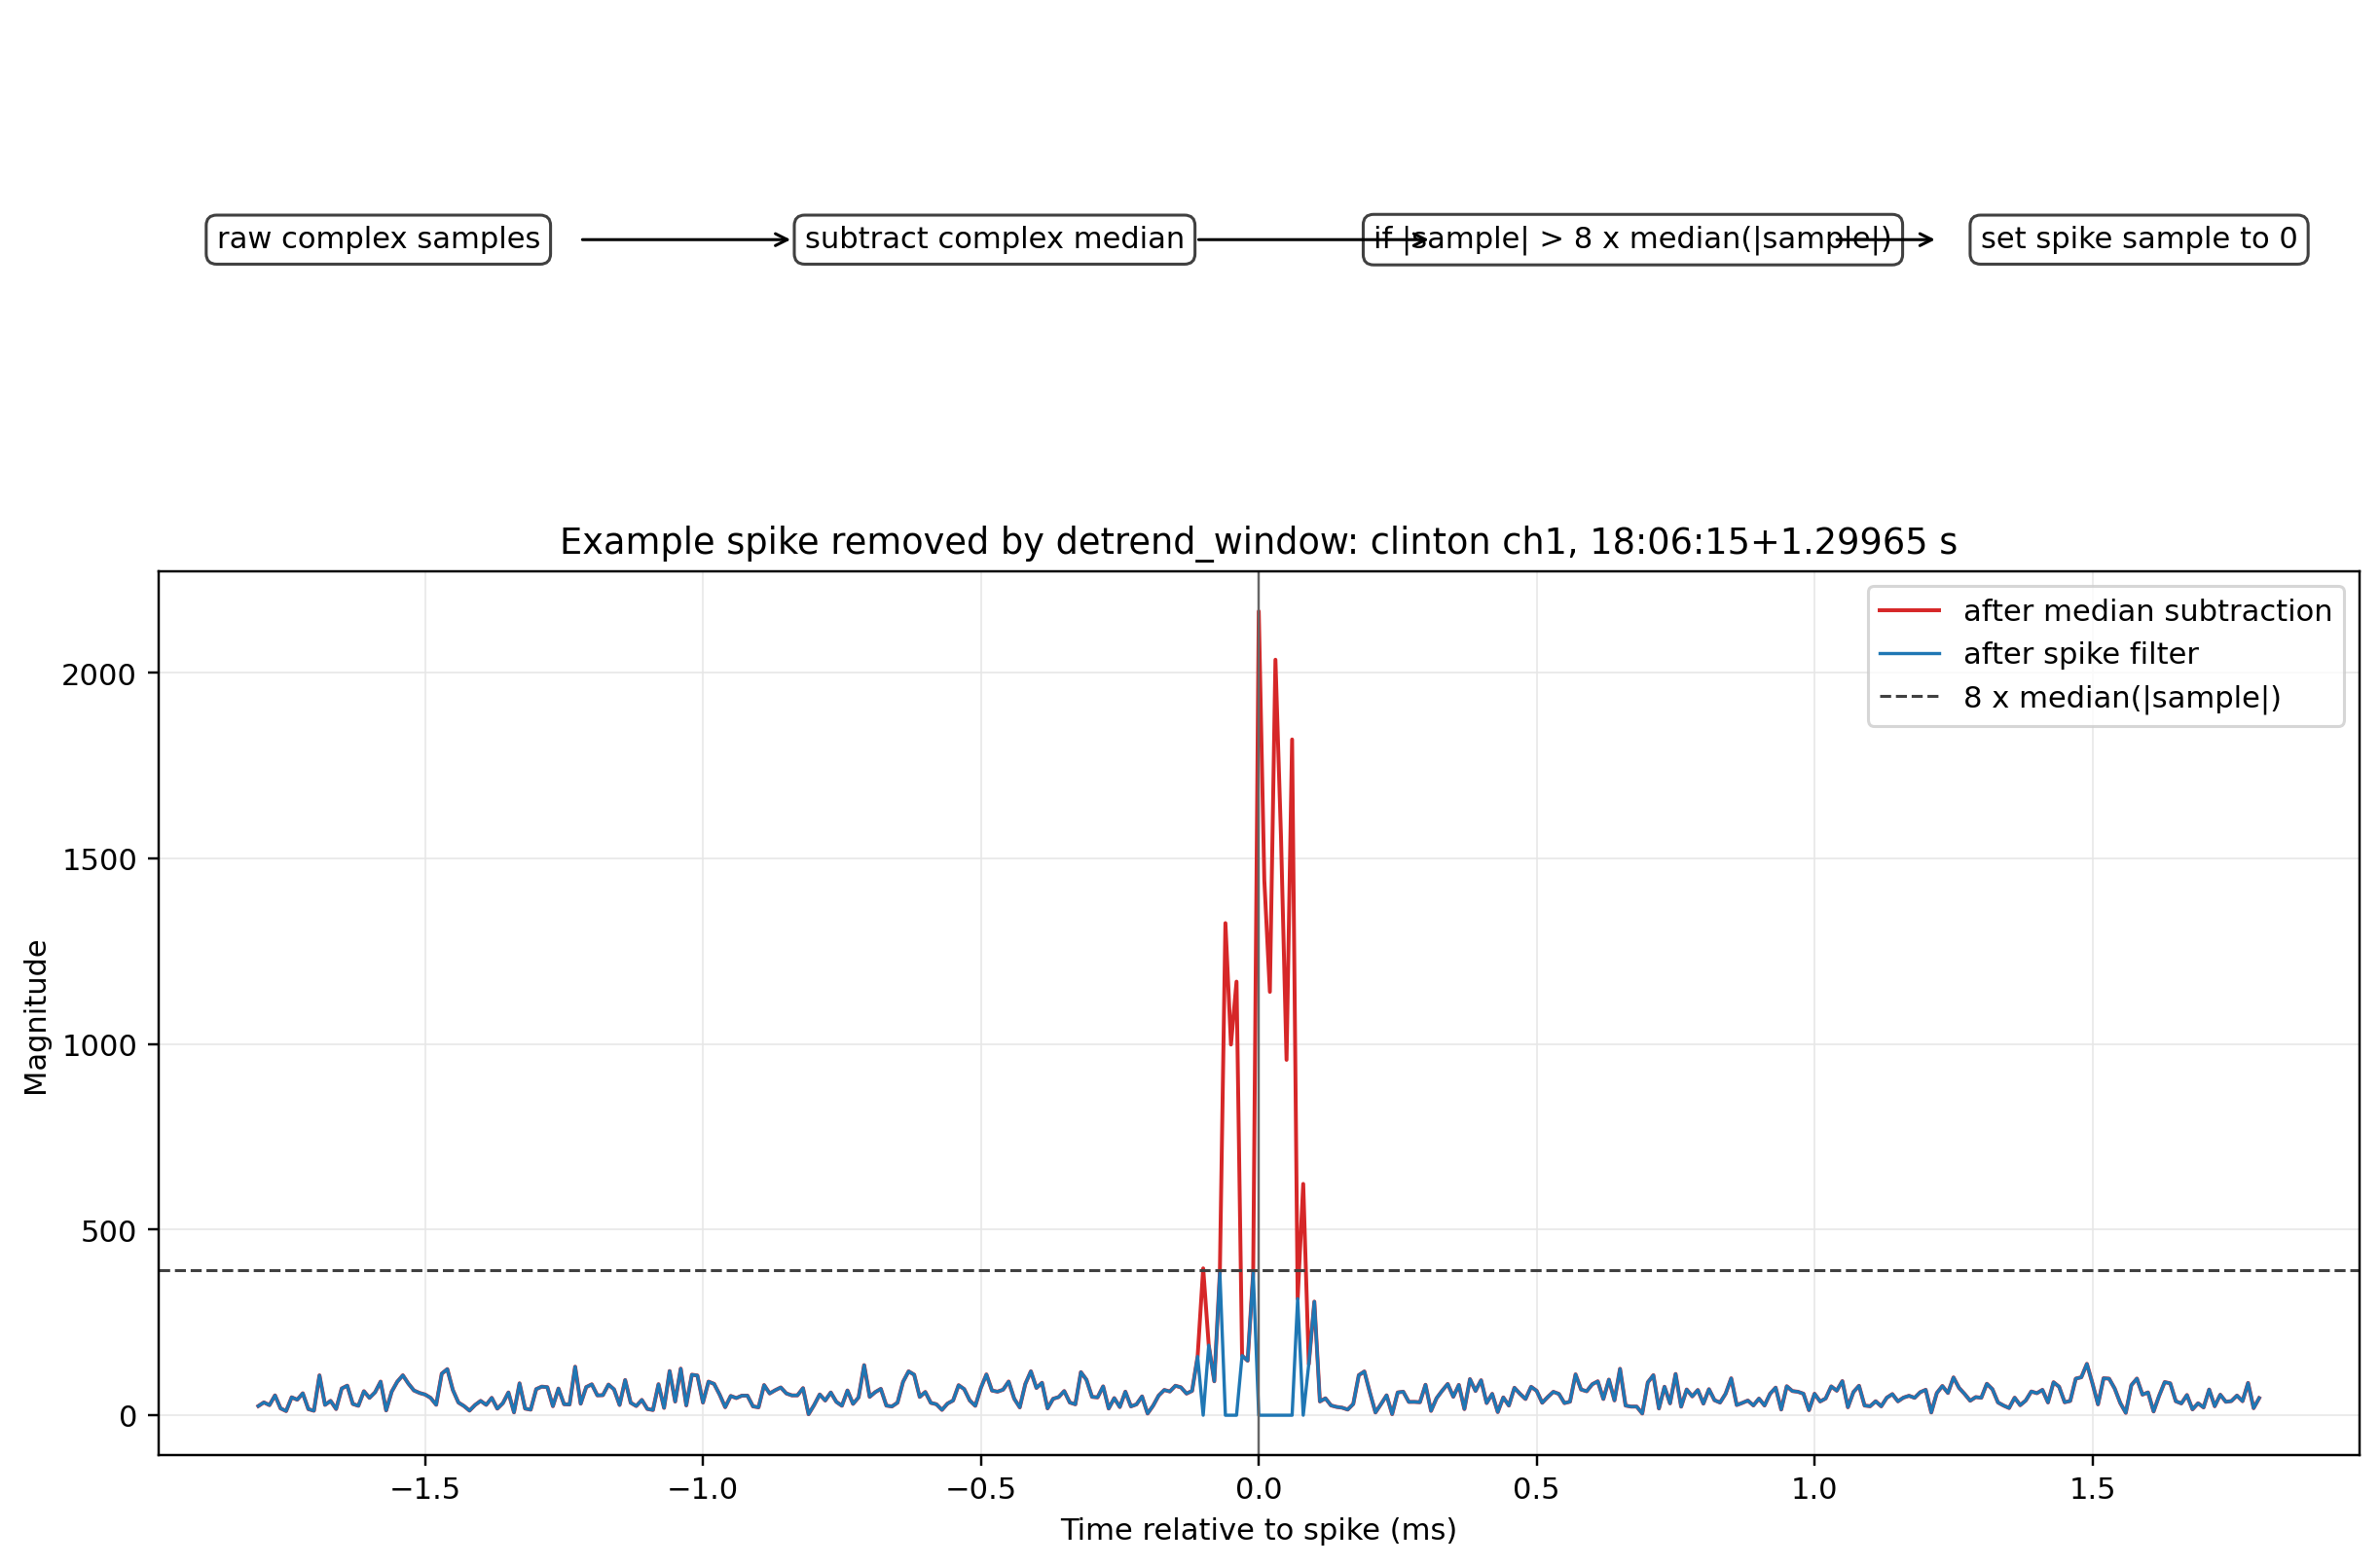
\includegraphics[width=\linewidth]{figures/detrend_window_spike_example.png}
  \caption{Diagnostic example of impulsive-sample excision.  The example is
  from \WorstSpikeStation{} channel \WorstSpikeChannel{} at
  18:06:15+\WorstSpikeOffset{} s.  Under the tested threshold, the largest
  sample is \WorstSpikeScore{} times the median absolute amplitude and would
  be set to zero after median subtraction.}
  \figsource{reports/generate_report_assets.py}
\end{figure}

For the 18:06:15--18:06:25 interval, using
\texttt{spike\_sigma=\SpikeSigma} across five stations and two receiver
channels would remove \SpikeTotalRemoved{} samples out of
\SpikeTotalSamples{} samples, or \SpikeFractionPercent.  The per-station
counts are:

\begin{center}
\begin{tabular}{lrrrr}
\toprule
Station & Channel & Samples & Removed & Fraction \\
\midrule
Amherst & 0 & 1,000,000 & 0 & 0.00000\% \\
Amherst & 1 & 1,000,000 & 0 & 0.00000\% \\
Beverly & 0 & 1,000,000 & 0 & 0.00000\% \\
Beverly & 1 & 1,000,000 & 0 & 0.00000\% \\
Clinton & 0 & 1,000,000 & 5 & 0.00050\% \\
Clinton & 1 & 1,000,000 & 12 & 0.00120\% \\
Pomfret & 0 & 1,000,000 & 0 & 0.00000\% \\
Pomfret & 1 & 1,000,000 & 0 & 0.00000\% \\
Siena & 0 & 1,000,000 & 0 & 0.00000\% \\
Siena & 1 & 1,000,000 & 0 & 0.00000\% \\
\bottomrule
\end{tabular}

\end{center}

The high-resolution matched-filter runs discussed here used no spike zeroing,
so the reported RTIs were not affected by this diagnostic excision.

Doppler whitening normalizes each Doppler bin by its median power over range:
\[
  S_{\mathrm{white}}(r,f) =
  \frac{S(r,f)}
       {\mathrm{median}_{r'}\,S(r',f)} .
\]
Peak selection is then performed on \(S_{\mathrm{white}}\), rather than on the
absolute power \(S\).  For this event the head echo is often not apparent in
the range--time product without this normalization, because
Doppler-dependent clutter and background structure can dominate the
absolute-power peak selection.  Whitening therefore emphasizes range gates
that are anomalously bright relative to other ranges at the same Doppler.

Figure~\ref{fig:beverly-whiten} shows a Beverly example at 18:06:20.600 UTC.
The example range gate was selected by searching 200--300 km for the maximum
whitened SNR with Doppler between \(-3000\) and \(-1000\) Hz.  The selected
gate is \BeverlyExampleRange{} km, with Doppler
\BeverlyWhitePeakDoppler{} kHz.  At this gate the selected bin has
\BeverlyRawSelectedSnr{} dB above the unwhitened range-gate median and
\BeverlySelectedSnr{} dB above the whitened range-gate median.  The diagnostic
illustrates the reduction of the Doppler-dependent background after division by
the median range power at each Doppler.

\begin{figure}[ht]
  \centering
  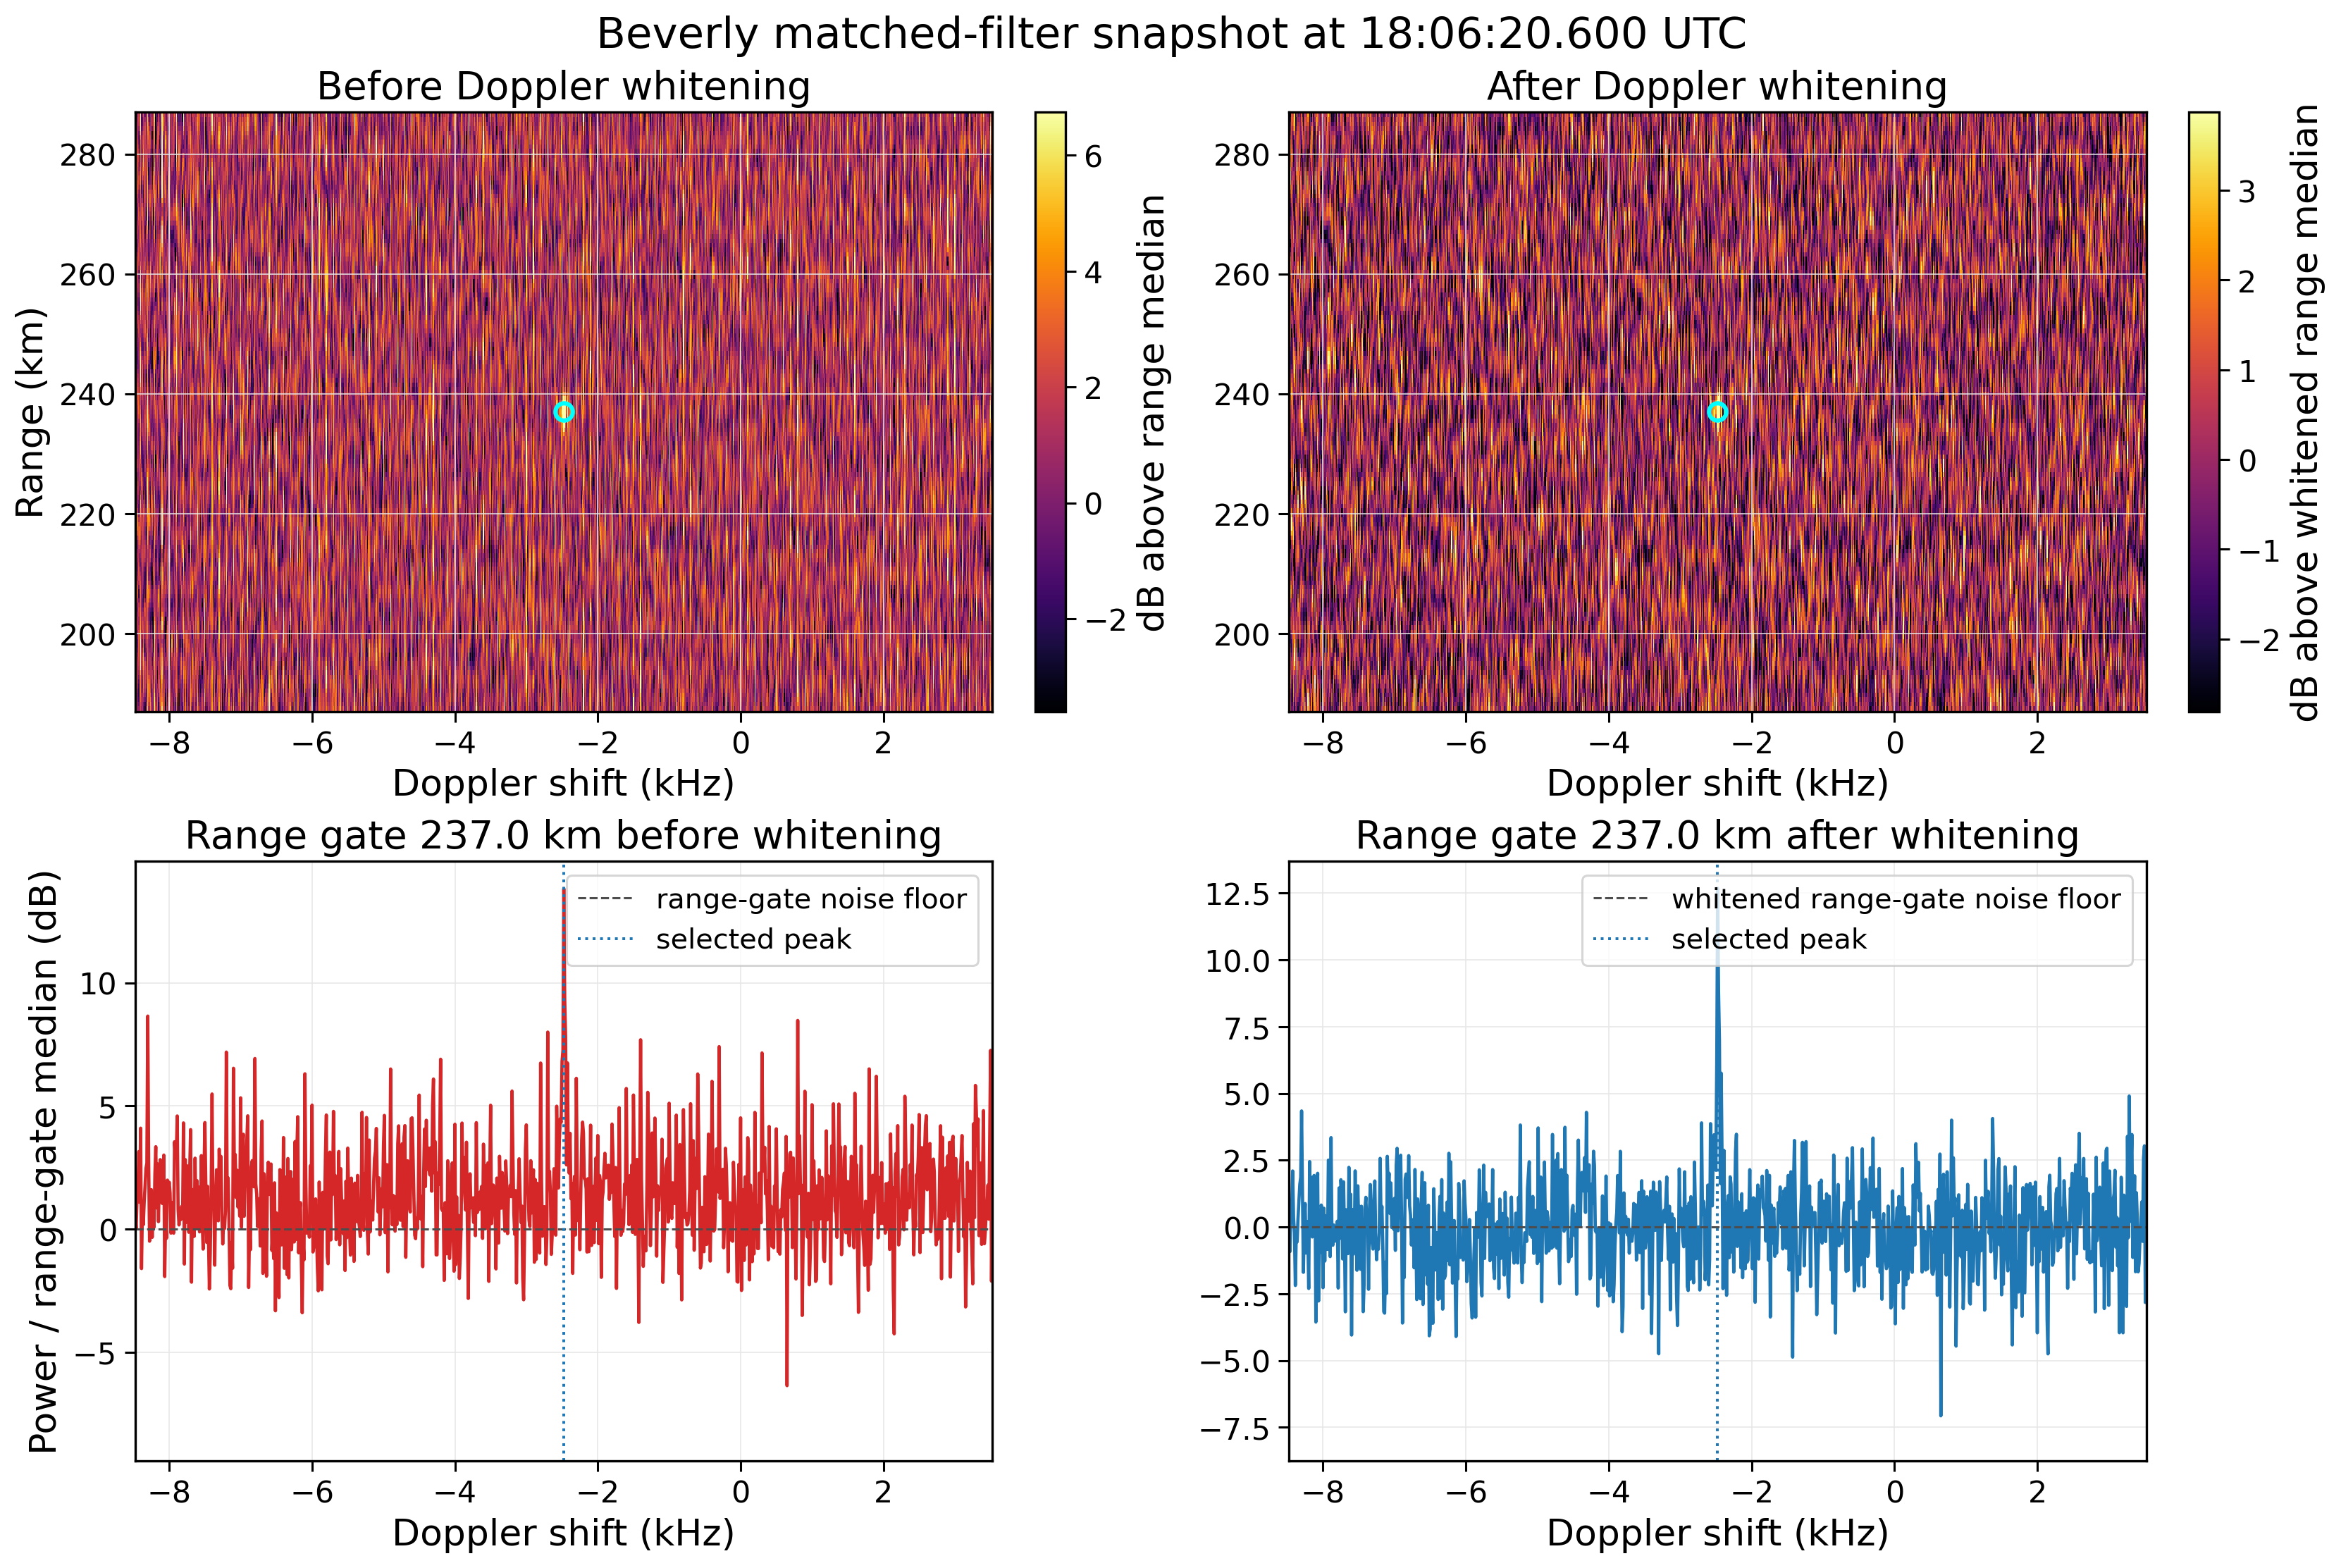
\includegraphics[width=\linewidth]{figures/beverly_doppler_whiten_example.png}
  \caption{Beverly range--Doppler snapshot at 18:06:20.600 UTC, before and
  after Doppler whitening.  The lower panels show the Doppler spectrum at the
  selected range gate and the corresponding range-gate noise floor.}
  \figsource{reports/generate_report_assets.py}
  \label{fig:beverly-whiten}
\end{figure}

\section{Coordinate-System Validation}
\label{app:coordinate-validation}

All reported positions are propagated through a single WGS84 geodetic,
Earth-centered Earth-fixed (ECEF), and local east--north--up (ENU) convention.
For a geodetic reference point at latitude \(\phi\) and longitude \(\lambda\),
the local ENU-to-ECEF rotation uses the columns
\[
\begin{aligned}
{\bf e} &= (-\sin\lambda,\cos\lambda,0),\\
{\bf n} &= (-\sin\phi\cos\lambda,-\sin\phi\sin\lambda,\cos\phi),\\
{\bf u} &= (\cos\phi\cos\lambda,\cos\phi\sin\lambda,\sin\phi).
\end{aligned}
\]
Thus \(R=[{\bf e}\ {\bf n}\ {\bf u}]\) is right-handed, with
\({\bf e}\times{\bf n}={\bf u}\).  Transmitter angle-of-departure vectors are
defined in this same ENU frame as
\[
{\bf \hat u}_{\mathrm{ENU}} =
(\sin A\cos E,\ \cos A\cos E,\ \sin E),
\]
where azimuth \(A\) is measured clockwise from north and elevation \(E\) is
positive upward.  The AoD plus bistatic-range position solve converts
\({\bf \hat u}_{\mathrm{ENU}}\) to ECEF, intersects the ray from the
transmitter with the ellipsoid of constant transmitter--target--receiver path
length, and stores the resulting ECEF, ENU, and geodetic coordinates.

Table~\ref{tab:coordinate-sanity} reports independent consistency checks run
on the current products.  These tests verify WGS84 round trips, ENU
orthonormality and handedness, azimuth/elevation cardinal directions, the
trajectory JSON's stored ENU/ECEF/geodetic fields, and all solved trail AoD
positions.  The residuals are at numerical roundoff level, far below the radar
range resolution and trajectory uncertainties.

\begin{table}[ht]
  \centering
  \caption{Coordinate-system sanity checks generated from the current trajectory
  and trail-position products.}
  \label{tab:coordinate-sanity}
  \small
  % Generated by tests/coordinate_sanity_checks.py --tex-out
\begin{tabularx}{\linewidth}{lXl}
\toprule
Check & Quantity & Maximum residual \\
\midrule
WGS84 geodetic $\rightarrow$ ECEF $\rightarrow$ geodetic & max altitude round-trip error & $2.24\times 10^{-9}$ m \\
WGS84 geodetic $\rightarrow$ ECEF $\rightarrow$ geodetic & max latitude/longitude round-trip error & $7.11\times 10^{-15}$ deg \\
ENU rotation matrix & max $|R^T R-I|$, $|\det R-1|$, and $|{\bf e}\times{\bf n}-{\bf u}|$ & $2.22\times 10^{-16}$ dimensionless \\
Azimuth/elevation unit vectors & max cardinal-direction unit-vector error & $1.84\times 10^{-16}$ dimensionless \\
Trajectory product & reference-state ENU/ECEF mismatch & $0$ m \\
Trajectory product & max stored model-series altitude mismatch & $1.86\times 10^{-9}$ m \\
Trail AoD positions & max ECEF/ENU/geodetic mismatch over 143 solves & $2.02\times 10^{-9}$ m \\
Trail AoD positions & max bistatic path-length residual & $1.34\times 10^{-9}$ m \\
Trail AoD positions & max AoD ray versus solved-position angular mismatch & $1.21\times 10^{-6}$ deg \\
\bottomrule
\end{tabularx}

\end{table}

\section{Trail Echo ROI Altitude Overlay}
\label{app:trail-roi-altitude-overlay}

\begin{figure}[ht]
  \centering
  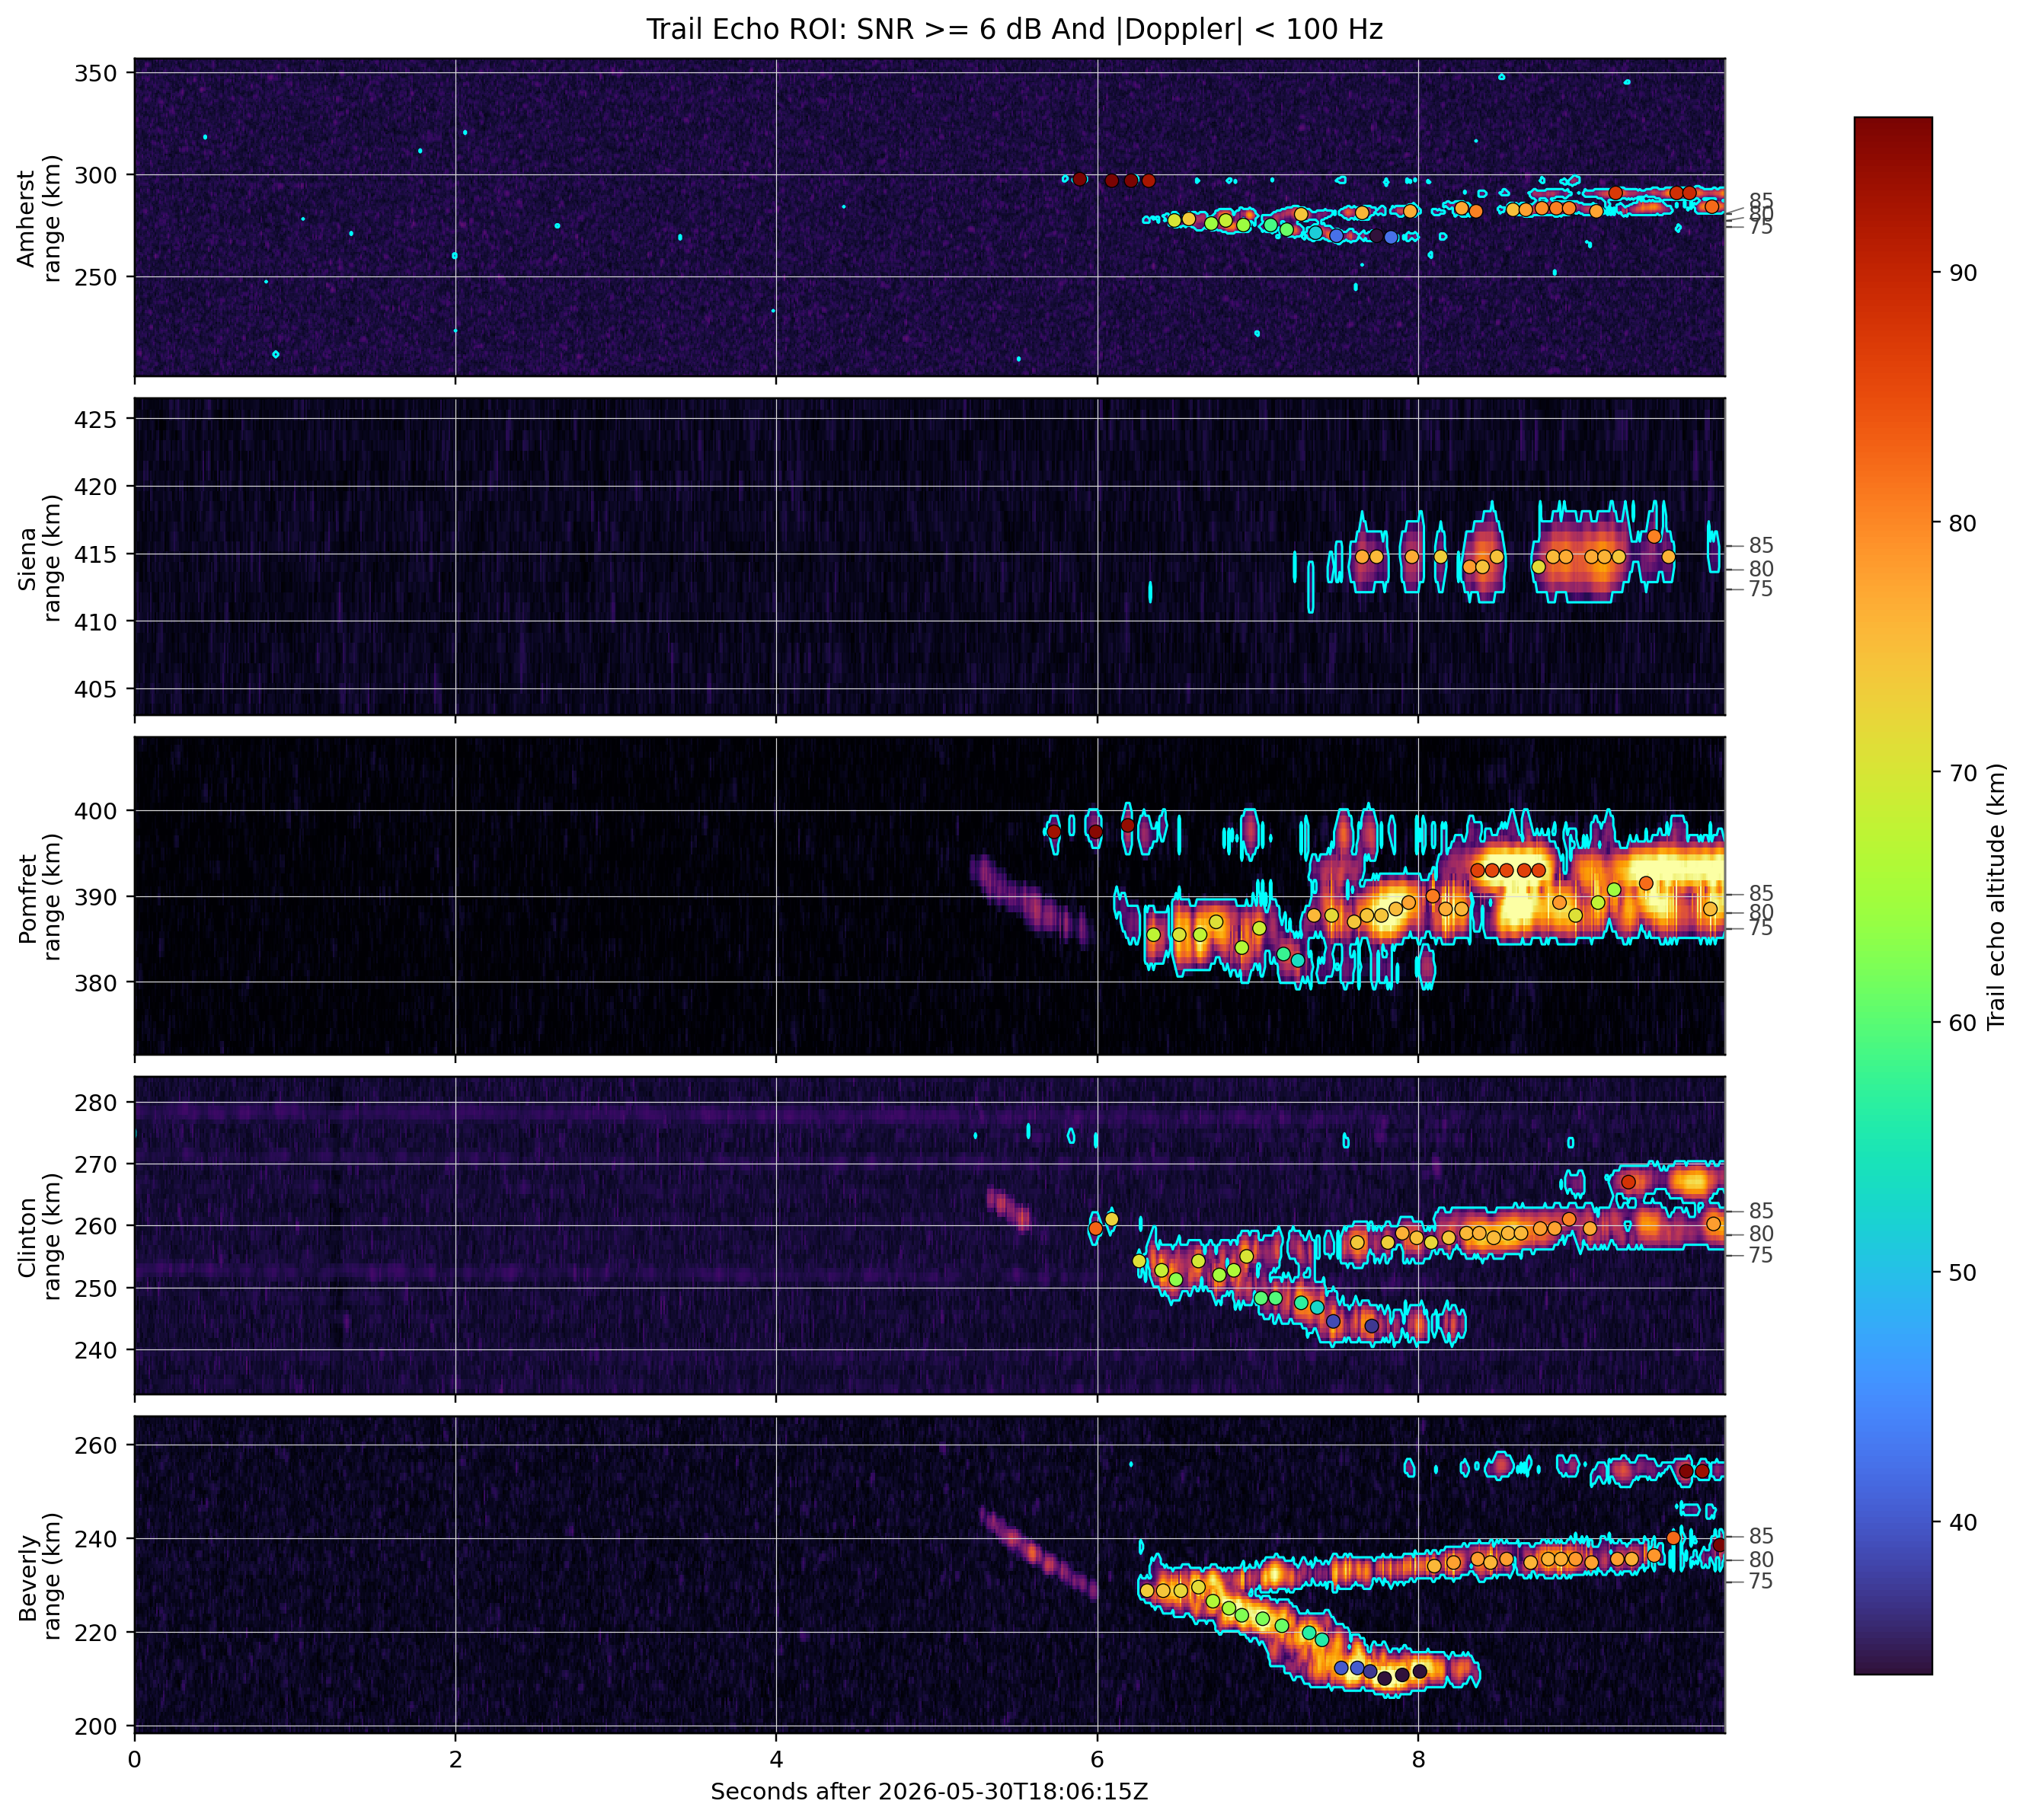
\includegraphics[width=\linewidth]{figures/trail_echo_roi_trail_altitude.png}
  \caption{Variant of Figure~\ref{fig:trail-echo-roi} with solved
  non-specular trail echo positions overlaid as scatter points.  Point color
  gives the AoD plus bistatic-delay altitude solution using a turbo color
  scale.}
  \figsource{trail_echo_roi.py}
  \label{fig:trail-echo-roi-trail-altitude}
\end{figure}

\section{GLM Follow-Up Context}
\label{app:glm}

GOES-19 Geostationary Lightning Mapper (GLM) data provide an independent data
source for this event.  Public reports noted a GLM optical burst over the
Massachusetts coast at approximately the same time as the reported sonic boom.
Although GLM is designed for lightning, bright bolide emission can appear as a
compact transient optical source in the lightning mapper.  For this event, the
GLM detection can be used as an external timing and geolocation constraint on
the luminous phase, complementary to the radar head-echo trajectory in
Figure~\ref{fig:ballistic-impact-map}.

The useful GLM products for follow-up are the event, group, and flash
locations and times near 18:06 UTC on 2026-05-30.  These should be compared
with the extrapolated radar trajectory, accounting for the GLM geolocation
uncertainty, cloud-top illumination geometry, and the fact that the optical
centroid need not coincide exactly with the radar head-echo scattering point.
In practice, the GLM burst can help reject trajectory solutions whose
extrapolated ground track misses the observed optical source region or whose
timing is inconsistent with the optical transient.

Infrasound and seismic observations are also likely to exist and should be
searched for follow-up analysis.  Large bolides can generate acoustic and
seismo-acoustic signals: direct atmospheric infrasound, ground-coupled acoustic
waves from sonic booms, and possible local shaking from fragmentation or airburst
overpressure.  Such observations would not replace the radar trail trajectory,
but they can provide independent timing, propagation-direction, and
fragmentation-sequence constraints.  In a joint interpretation, the radar head
echo gives the moving scattering point, the non-specular meteor-radar trail
positions give the spatial line left behind in the atmosphere, GLM constrains
optical emission, and infrasound/seismic arrivals can constrain when and where
the main acoustic energy was deposited.

The first search should use regional open seismic networks in and near New
England.  Relevant archives include the New England Seismic Network operated
through Weston Observatory/Boston College and distributed through the USGS/ANSS
and EarthScope/IRIS data systems, the Lamont-Doherty Cooperative Seismographic
Network in New York and adjacent states, and Canadian seismic stations in
Quebec and the Maritime Provinces.  Stations closest to Cape Cod Bay and coastal
Massachusetts should be inspected for 18:06 UTC plus the expected acoustic
propagation delay.  The useful signal may be a low-frequency airwave or
ground-coupled arrival rather than a normal earthquake-like phase, so waveform
inspection and array/back-azimuth methods are preferable to relying only on
standard earthquake event catalogues.

The Comprehensive Nuclear-Test-Ban Treaty Organization International Monitoring
System (IMS) should also be checked as a long-range infrasound/seismic context
network.  The IMS includes a global 60-station infrasound array network and
primary/auxiliary seismic stations designed for nuclear-test monitoring but
also sensitive to natural and anthropogenic events, including meteors
\cite{ctbto_infrasound_monitoring,ctbto_ims_map}.  For this event, candidate
IMS infrasound stations to query include I10CA at Lac du Bonnet, Manitoba,
IS53 near Fairbanks, Alaska, and IS18 at Qaanaaq, Greenland; these are not local
New England sensors, but long-range infrasound can propagate thousands of
kilometres depending on stratospheric winds.  Candidate IMS seismic context
stations in northeastern North America include PS8 Lac du Bonnet, PS9
Yellowknife, and PS10 Schefferville, Quebec.  Access to some IMS waveform data
may require CTBTO/IDC channels, but station metadata and public descriptions
are useful for planning the search
\cite{nrcan_ims_infrasound,ctbto_station_profiles}.

\printbibliography

\end{document}
